\chapter{Swarm coordination - perimeter detection}\label{chapter:coordination}
%% \section{Introduction}
This chapter identifies the effect a \textit{destination vector} has upon the motion of a swarm. Three coordination techniques are applied to a swarm and the metrics defined in chapter~\ref{chapter:metric} are used to identify the effects. The three coordination techniques are: full perimeter detection, where only edge based agents will have a \textit{destination vector} applied, partial perimeter detection, where a subset of the perimeter agents are detected and finally all agents in the swarm having a \textit{destination vector} applied. For all the experiments the base parameters of the swarm are fixed ensuring that the only variable will be the \textit{destination vector} that is applied by the coordinating agents. This process allows the impact of the algorithms to be isolated and compared. Section~\ref{sec:AlternateBias1}~discusses the potential variations to the base parameters and the effects this has on controlling the impact of the weightings.

\section{Baseline specification}
To allow an analysis of each algorithm's effect on a swarm a baseline measurement of `background' variance (jitter) is identified. The baseline measurement provides a comparative data set for the experiments. The baseline data set is for a static swarm (no destination vector) with the same internal parameters.

\textit{Assumption 1:} The swarm used for the experiments consists of 200 agents randomly distributed~(Figure~\ref{fig:SampleSwarm200-1}).\\ 
\textit{Assumption 2:} The field effects and bias will be set as shown in~Table~\ref{tab:DynamicPhysics1} with the weight adjuster $k_d = 0$ for the baseline.\\
\textit{Assumption 3:} All destination based experiments will have the weight adjuster set to $k_d = 100$.

\begin{figure}[H]
\begin{center}
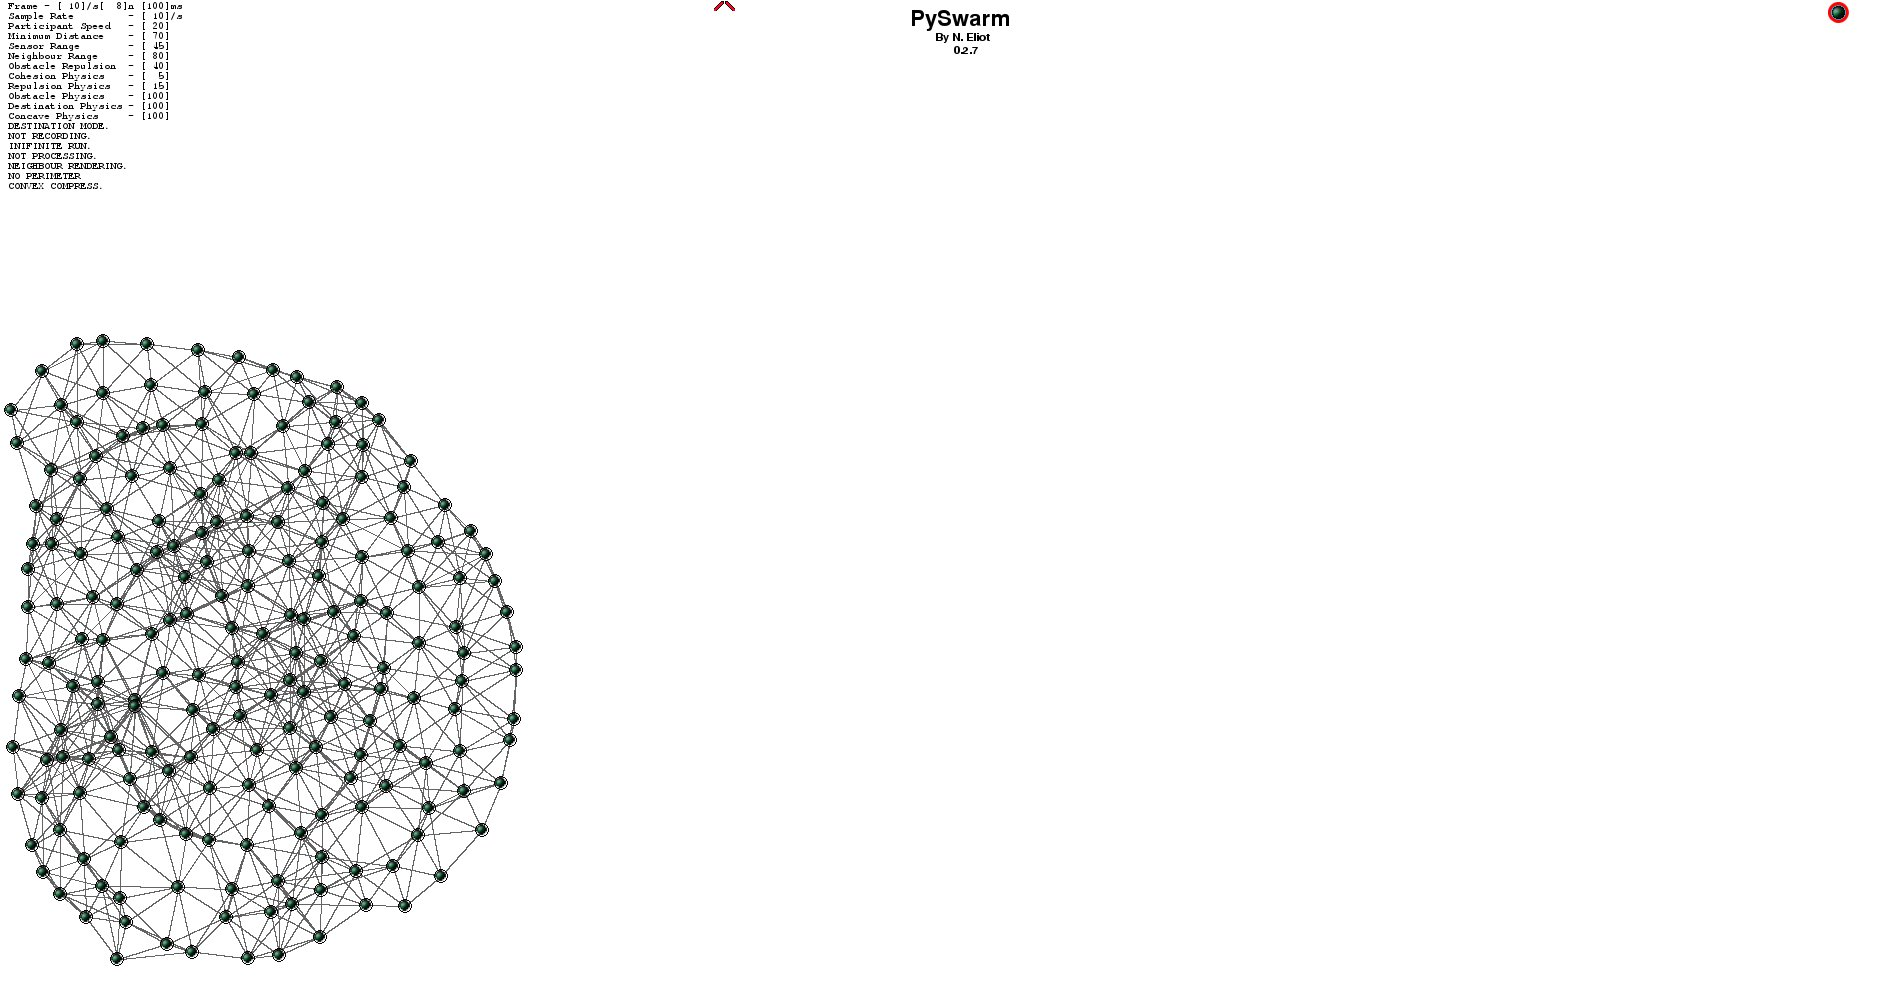
\includegraphics[width=14cm]{CHAPTER-6/figures/SampleSwarm200-1}
\end{center}
\caption[Sample swarm 200 agents initial state]{Sample swarm 200 agents initial state (\textit{screen shot from simulator})\label{fig:SampleSwarm200-1}}
\end{figure}

\begin{table}[H]
\begin{center}
\begin{tabular}{| p{2.5cm} | c | p{7cm} |}
\hline
\bf Weight \bf Component & \bf \swarmA{} & \bf Description \\ \hline
Sample Rate & 100 & ms - Unit sampling interval\\  \hline
$k_c$ & 5 & weight adjuster for cohesion vector\\  \hline
$k_r$ & 15 & weight adjuster for repulsion  vector\\  \hline
$k_d$ & 0/100 & weight adjuster for destination vector 0 for static baseline 100 for destination based\\  \hline
Repulsion field & 70 & units\\  \hline
Cohesion field & 80 & units\\  \hline
Speed & 20 & units/s\\  \hline
\end{tabular}\caption{Swarm Weighted Model} \label{tab:DynamicPhysics1}
\end{center}
\end{table}

The results for the baseline experimental swarm are shown in~Table~\ref{coord:BaselineMagnitude1} and~\ref{coord:BaselineDistance1}. The metrics used are the distance \cite{NIM:09} and resultant inter-agent magnitudes (\textit{inter-agent vector}).

\begin{figure}[H]
\begin{center}
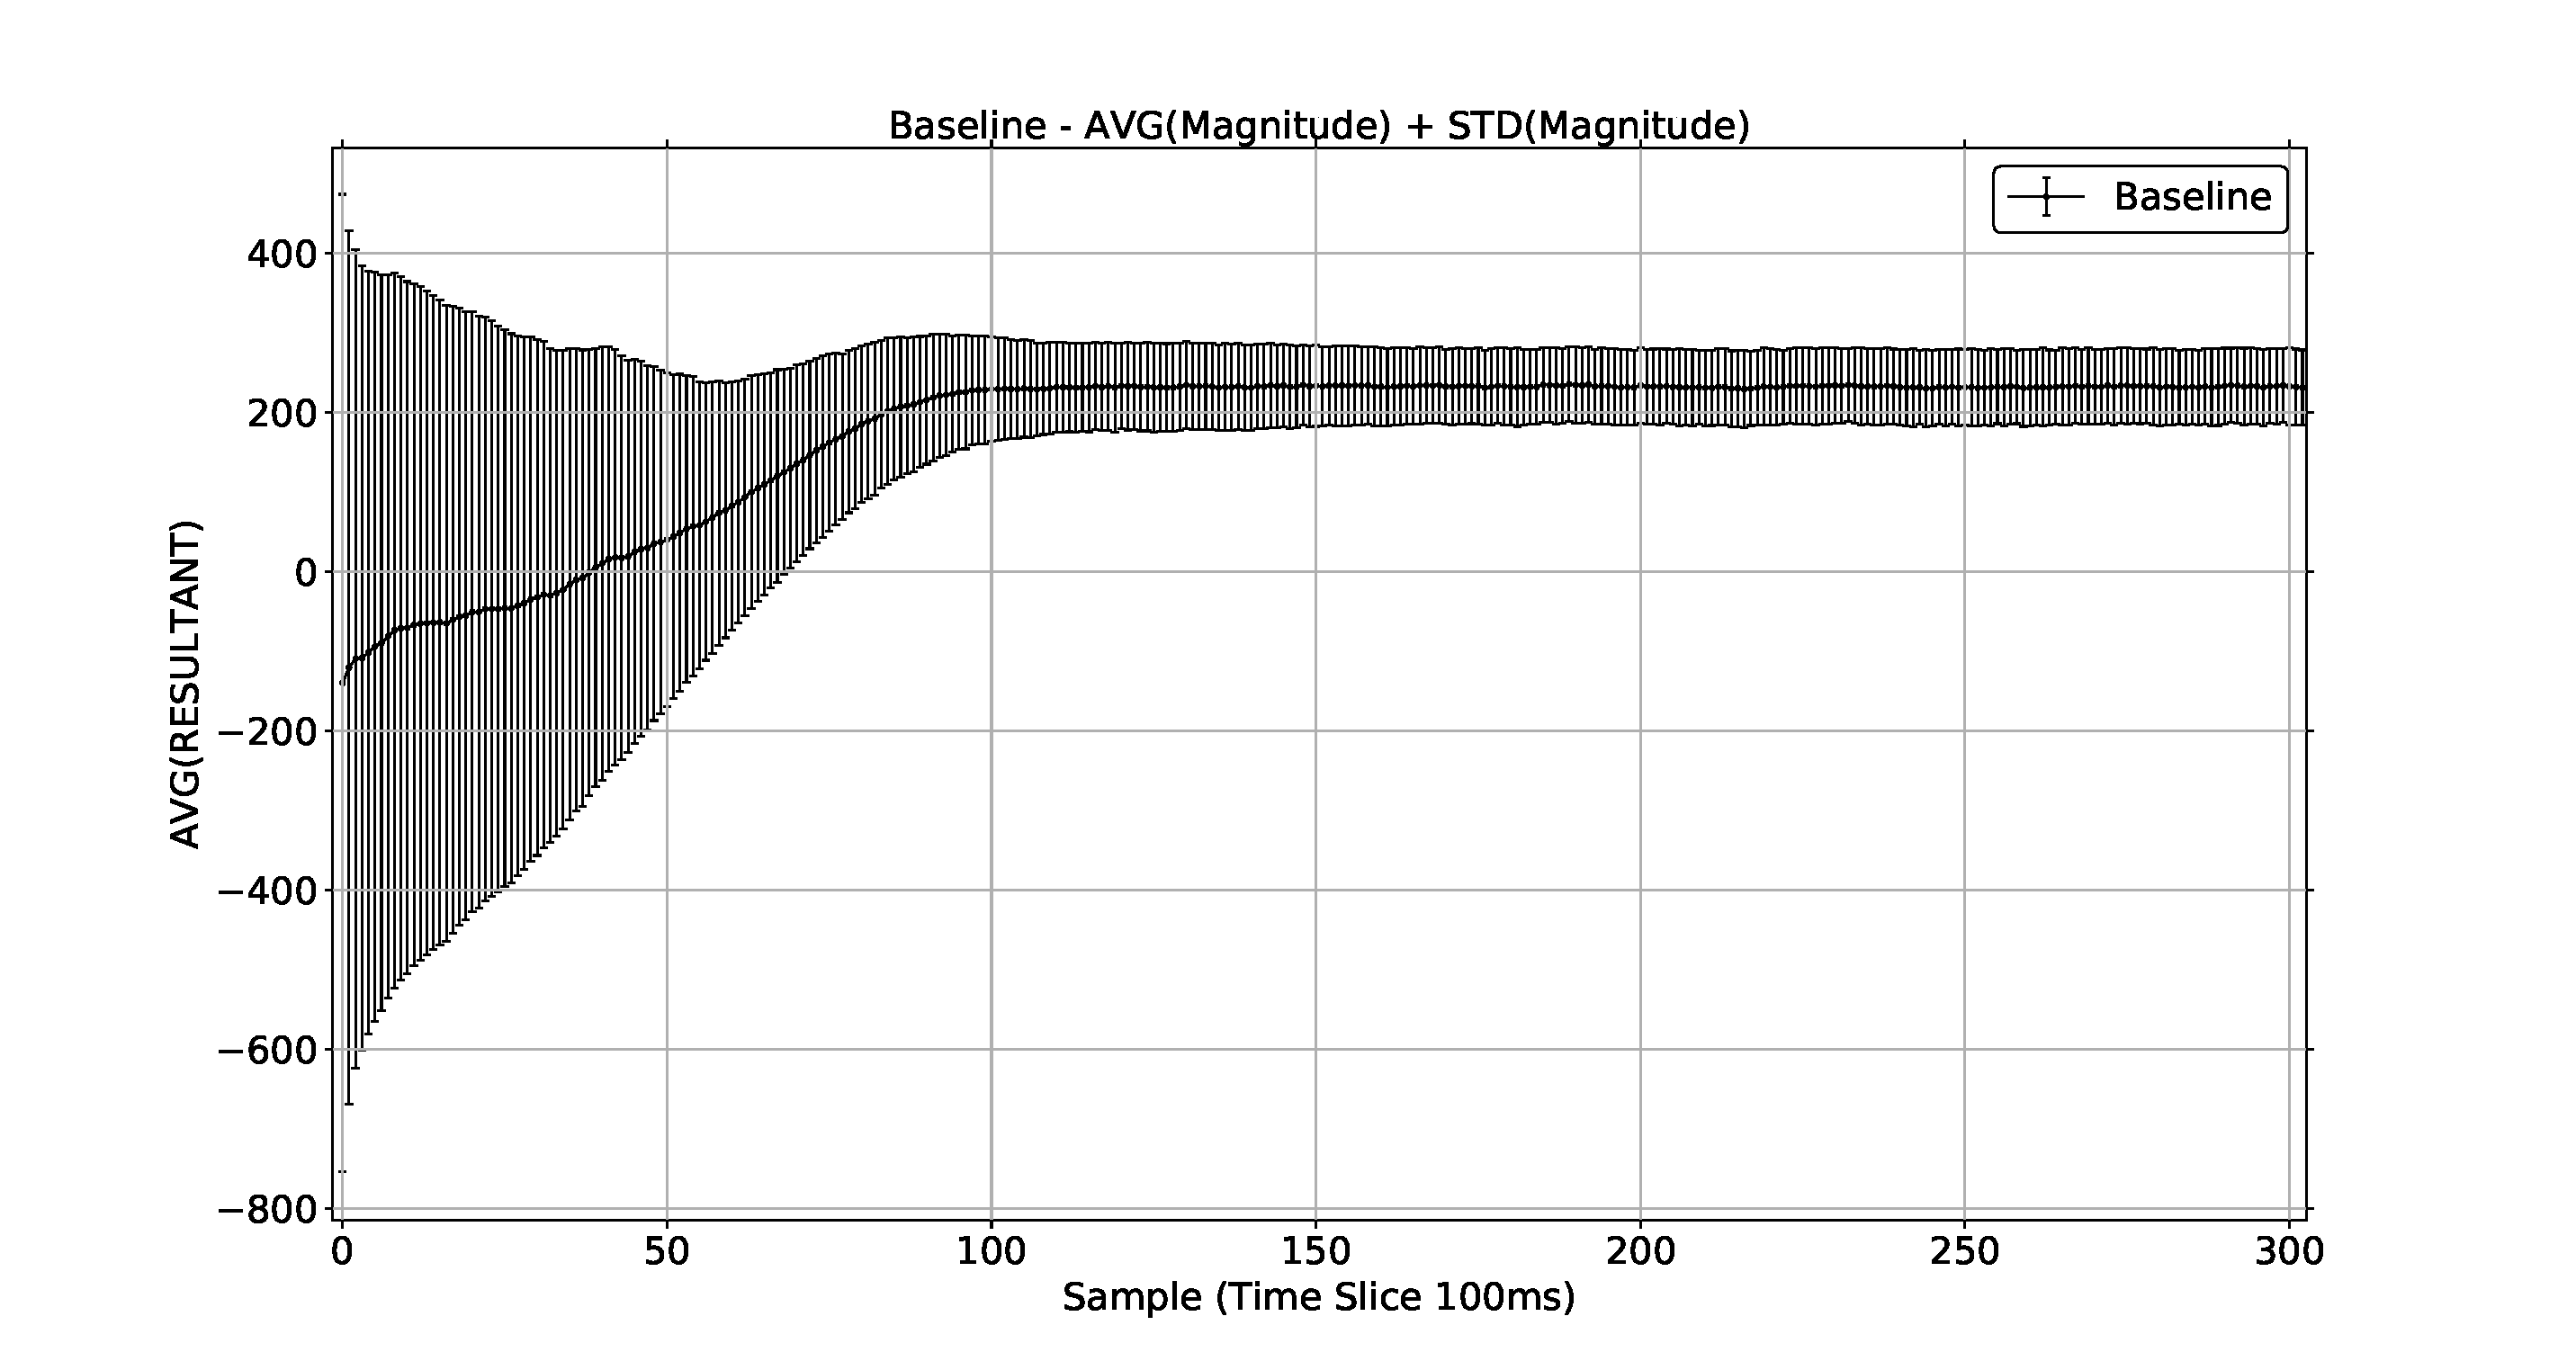
\includegraphics[width=14cm]{CHAPTER-6/figures/BaselineMagnitude1}
\end{center}
\caption{Baseline internal movement - magnitude\label{coord:BaselineMagnitude1}}
\end{figure}

Figure~\ref{coord:BaselineMagnitude1} shows the magnitude between $t_0$ and approximately $t_{48}$ dominated by repulsion ($|k_rv_r| > |k_cv_c|$). This indicates that the swarm is undergoing a rapid expansion as the bias within the swarm shows a high level of repulsion. Between approximately $t_{48}$ and $t_{100}$ the magnitude is positive but rising which indicates the swarm is cohesive and will remain a cohesive unit but it is still expanding. At approximately $t_{110}$ the swarm has completed it's expansion and has reached a settled state with the `background' movement maintaining the swarm's structure with $|k_rv_r| < |k_cv_c|$. The residual `jitter' is at its minimum for the configuration and the agent distribution is at its optimum for the cohesion and repulsion settings. The resultant $|k_rv_r| < |k_cv_c|$ is due to the cohesion field being larger than the repulsion field which prevents the swarm `breaking up'. 

\begin{figure}[H]
\begin{center}
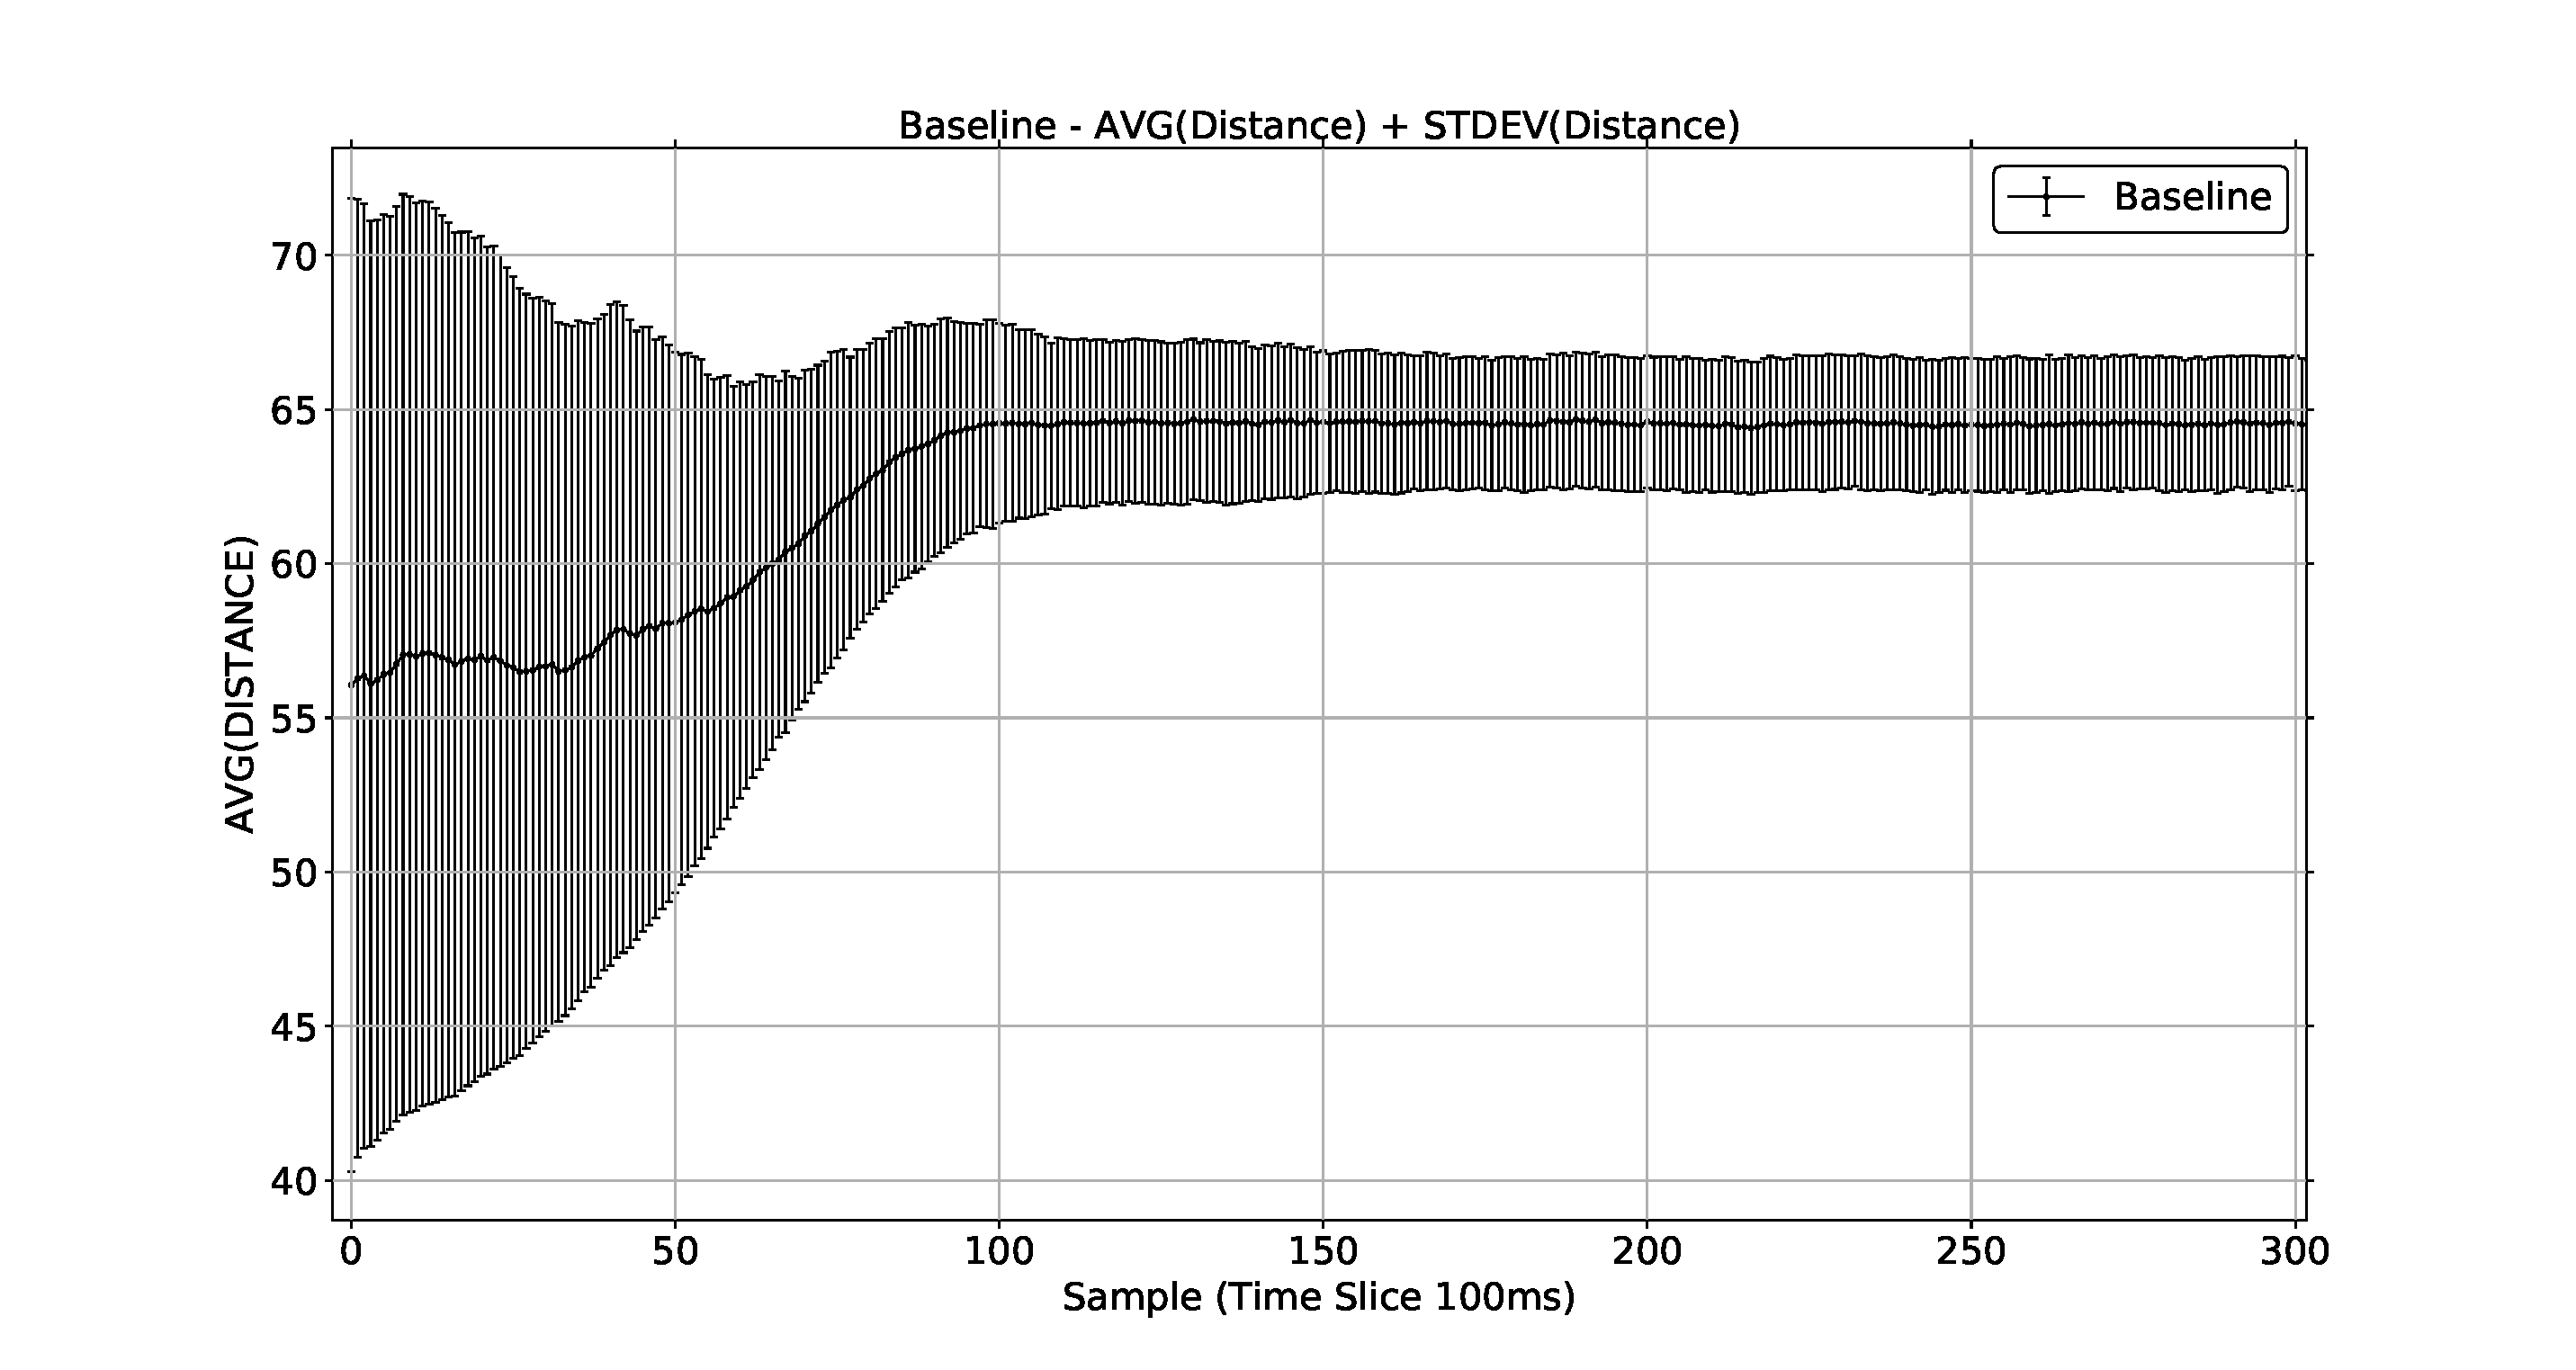
\includegraphics[width=14cm]{CHAPTER-6/figures/BaselineDistance1}
\end{center}
\caption{Baseline internal movement - distance\label{coord:BaselineDistance1}}
\end{figure}

Figure~\ref{coord:BaselineDistance1} shows the internal movement and the deviation from the mean for the swarm based on the inter-agent distances. There is no \textit{destination vector} applied so all internal movement is being generated by the cohesion and repulsion vectors. The swarm is initially in a disorganised state but once the agents have expanded a stable hexagonal formation evolves. Figure~\ref{coord:BaselineDistance1} shows the first 30s of the simulation which is sufficient time for the swarm to `settle' and transform to its most stable state. Due to the metric only showing inter-agent distances it is not possible to determine if the swarm will remain cohesive.

The centroid path for the baseline swarm is shown in~Figure~\ref{coord:SwarmPathBaseline1}. Due to there being no \textit{destination vector} for the swarm the centroid changes positions based on the inter-agent positional changes caused by the \textit{interaction vectors}. These changes are the result of each agents attempting to attain a state of equilibrium within their `clusters'.

\begin{figure}[H]
\begin{center}
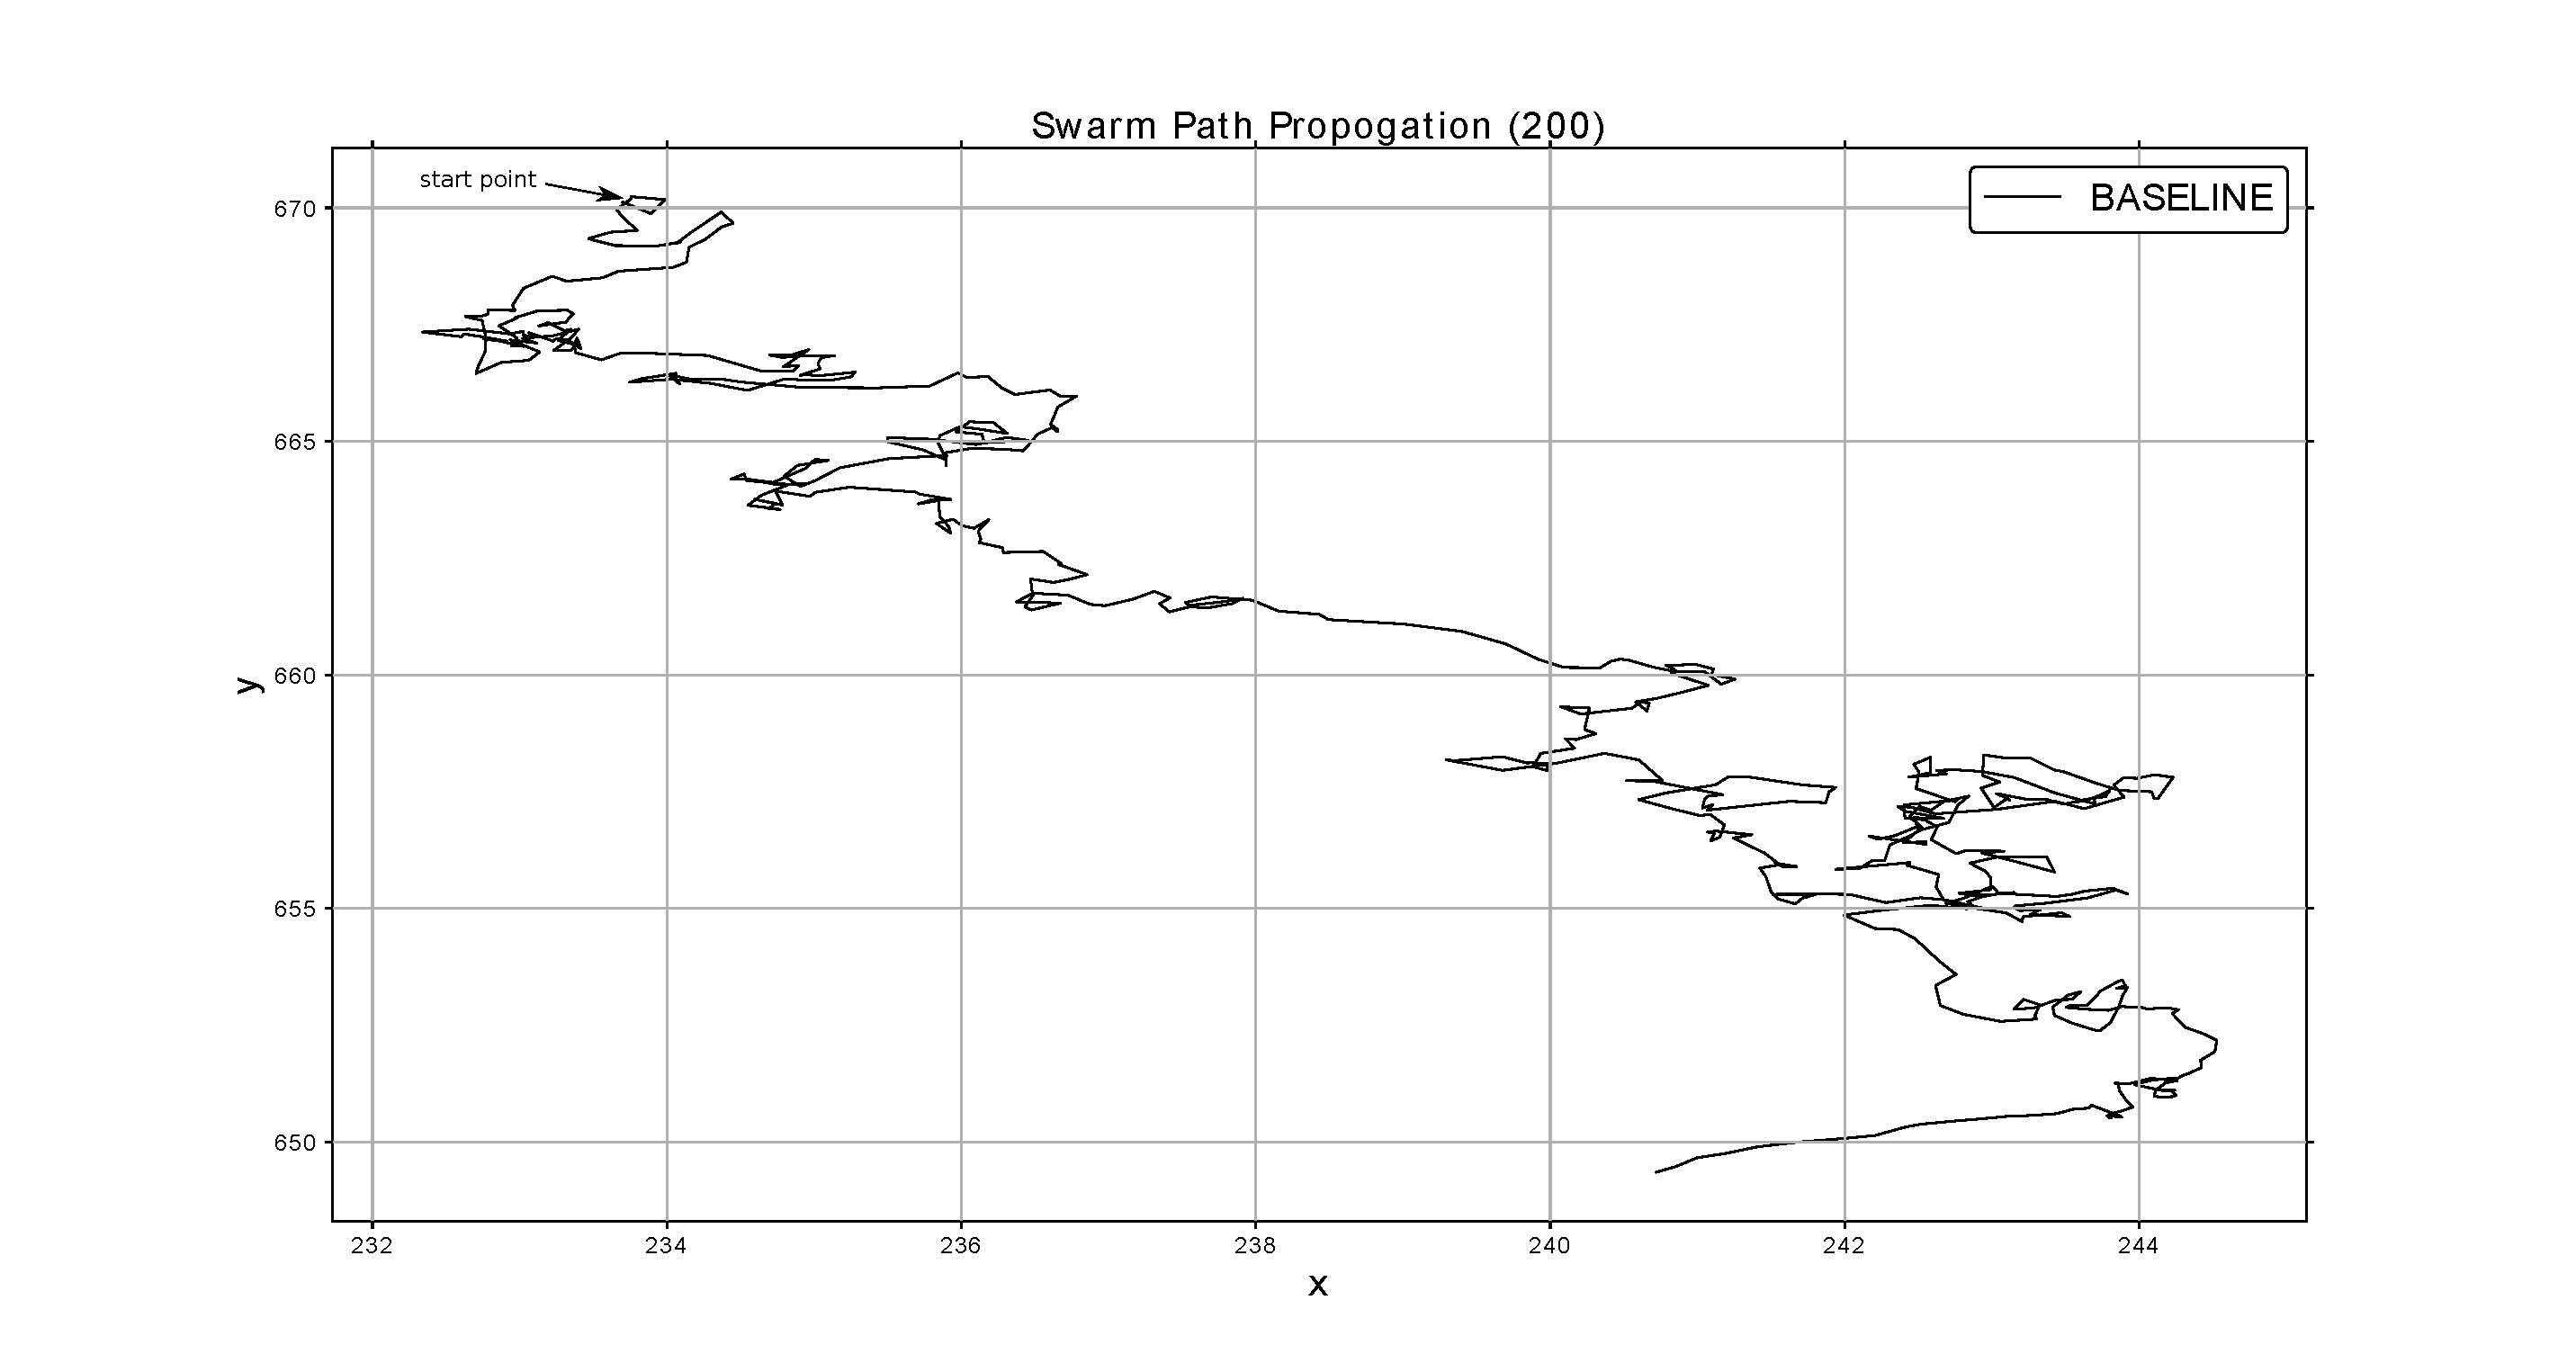
\includegraphics[width=14cm]{CHAPTER-6/figures/SwarmPathBaseline}
\end{center}
\caption{Baseline swarm path\label{coord:SwarmPathBaseline1}}
\end{figure}

These baseline measurements are used to identify the changes that occur in the structure of a swarm when changes are made to the weightings of the field effects, the number of coordination agents and the \textit{destination vector} weighting.

\section{Destination vector application}
Many mechanisms can be used to influence a swarm to travel in a specific direction. These mechanisms generally involve the use of sensors such as magnetometers or GPS's to achieve a directional coordinate \cite{SG:15,TG:12}. 

This thesis aims to produce algorithms that will reduce the number of active sensors that are needed for the directional coordination of a swarm. When reducing the number of active sensors the algorithms must maintain sufficient coordination of agents to influence the swarm's direction and therefore create an overall \textit{destination vector} to a swarm's movement. Reducing the number of active sensors will reduce the net energy usage of the sensors and potentially increase the sensors viable lifetime. Another aspect of the algorithms is that they should minimise the internal disturbance (jitter) created by the \textit{destination vector}.

There are two distinct approaches to configuring agents: all the agents are configured identically (homogeneous swarm) or the agents are in a selection of different configurations (heterogeneous swarm)~\cite{BS:13}. 

The following assumptions are made in this thesis:

\textit{Assumption 1:} All agents are identical (homogeneous) but are able select subsystems as necessary and adopt different roles depending upon the algorithm being used to coordinate the swarm. \\
\textit{Assumption 2:} As the swarm progresses towards a destination the role of an agent can change such that all the agents are identical in construct but they can enable and disable sensors as necessary. This will allow agents within the swarm to self promote to the coordinator role should a set of conditions arise.\\
\textit{Assumption 3:} All agent in the swarm are autonomous and each agent has its own power supply. 

Reducing the usage of sensors will reduce the net power consumption of the swarm and increase the time that an agent can be a part of a swarm. If the purpose of the swarm is reconnaissance then the reduction in energy usage may allow a longer traversal time, or allow the swarm to travel further. As agents in the swarm will use their resources at different rates some agents may be lost due to resource exhaustion. The algorithms should therefore be resilient to this.

\section{Swarm destination vector}
The following assumptions are made in this thesis:

\textit{Assumption 1:} The direction of the swarm is based upon having a fixed goal that is known to all the agents (\autoref{sec:Direction1}). \\
\textit{Assumption 2:} The goal is migrated towards based on a simulated GPS signal and the bias $k_d$ is applied to the \textit{destination vector} to influence the movement of the agents. 

The swarm's destination is established by the coordinator agents influencing the non-coordinator agents. This influence is applied through the coordinators proximity to non-coordinator agents (cohesion). Coordinator agents are identified by a set of conditions. The conditions are the activators for the coordinator identification algorithms.

\section{Identifying the coordinator role}
For an agent to change its role from a standard agent to a coordinator there needs to an algorithm that identifies a set of conditions to trigger the change. This same algorithm also triggers an agent to revert to being a standard agent. The coordinator selection algorithm is separate from the agent coordination algorithms discussed in chapter~\ref{chapter:methods}.

In this thesis three algorithms are presented and compared. In the first algorithm, all agents have the role of a coordinator permanently. This will be referred to as the all-agent algorithm. The other two mechanisms employ a selection criteria to identify if the simulated GPS sensor should be enabled. These two algorithms are: full-perimeter detection and the partial perimeter detection. Partial perimeter detection will be referred to as the basic-count algorithm.

There are many other ways in which the coordinator role could be established such as randomly enabling a GPS for a set period of time or oscillating the role on and off but they are beyond the scope of this thesis.

\section{Monolithic swarm - (all-agent)} 
In a monolithic swarm \cite{BS:13} the propagation towards the goal is achieved by all the agents using a GPS signal to give each agents' movement a \textit{direction vector} towards a required goal~(Equation~\ref{eq:BotDirection1}). There is no selection criteria and no computational overhead for the agents.

Figure~\ref{reduced:Monolithic1} shows a screen shot from the swarm simulator with all agents GPS's enabled. This can be seen as the agents highlighted with a ring around them. The small `tail' on each agent is the \textit{movement vector}.

\begin{figure}[H]
\begin{center}
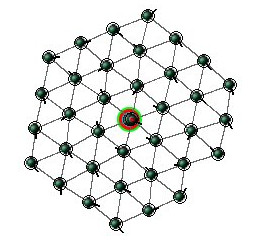
\includegraphics[width=7cm]{CHAPTER-6/figures/Monolithic2}
\end{center}
\caption[Monolithic agents]{Monolithic agents (Circles indicate all agents are using GPS, \textit{screen shot from simulator}) \label{reduced:Monolithic1}}
\end{figure}

\subsection{Baseline and effect of no perimeter detection\label{section:compareBaselineNoPerimeter}}
To identify the effect of the all-agents algorithm the simulation is executed using the same parameters as the baseline swarm with the added \textit{destination vector} on all the agents. The effect of introducing this bias on the swarm's internal characteristics can be seen in~Figures~\ref{reduced:BaselineAllAgentsMag1} and~\ref{reduced:BaselineAllAgentsDist1}.
%BASELINE-ALLAGENTS-MAG.py
\begin{figure}[H]
\begin{center}
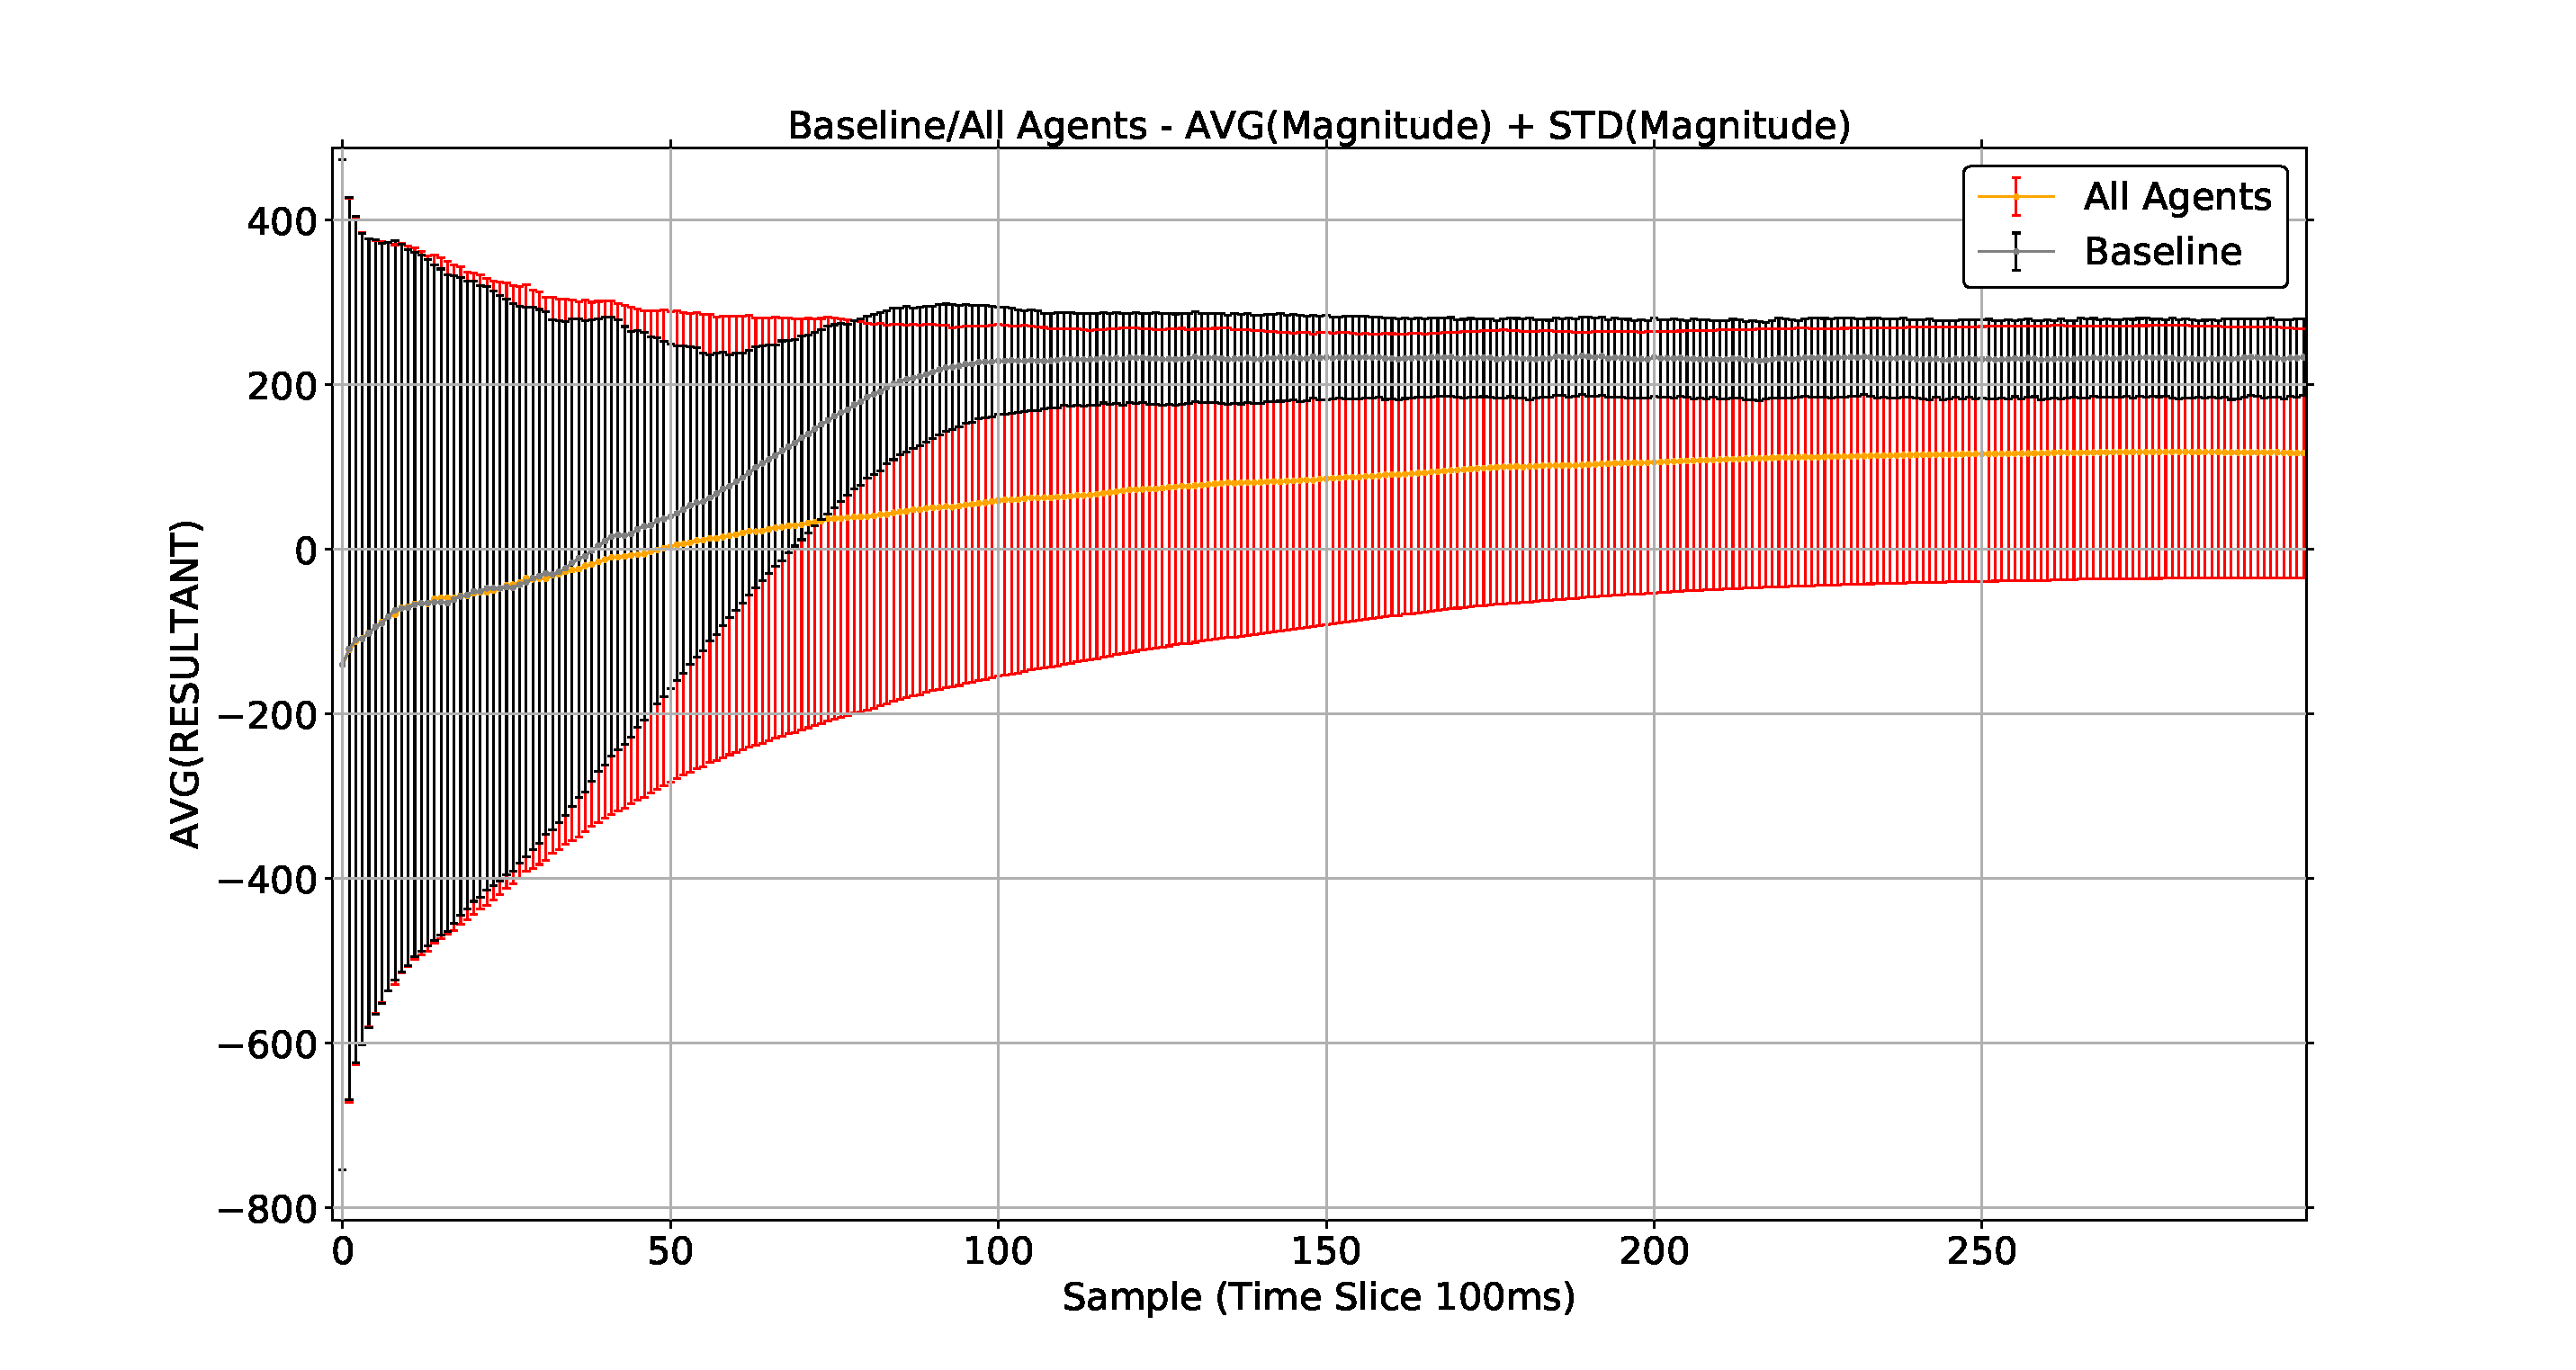
\includegraphics[width=14cm]{CHAPTER-6/figures/BaselineAllAgentsMag1}
\end{center}
\caption{Baseline/All agents comparison \textit{inter-agent vector} magnitude\label{reduced:BaselineAllAgentsMag1}}
\end{figure}

Figure~\ref{reduced:BaselineAllAgentsMag1} shows the effect on the \textit{inter-agent vector} magnitude of the swarm: the average resultant magnitude is lower than the baseline. This is due to there being a greater distribution of \textit{inter-agent vector} magnitudes from the disturbance caused by the \textit{destination vector} on all of the agents and the swarm is therefore less cohesive. The graph also shows that there is a higher variation from the mean; again this is due to the change in the bias of all the agents. The agents are moving towards a goal and are therefore not moving to an equilibrium distribution. Figure~\ref{reduced:BaselineAllAgentsMag1}~also shows that the \textit{direction vector} increases the time it takes for the swarm to distribute the agents and although the deviation diminishes the swarm cannot overcome the \textit{direction vector's} effect and the swarm appears disorganised.
%BASELINE-ALLAGENTS-DIST.py
\begin{figure}[H]
\begin{center}
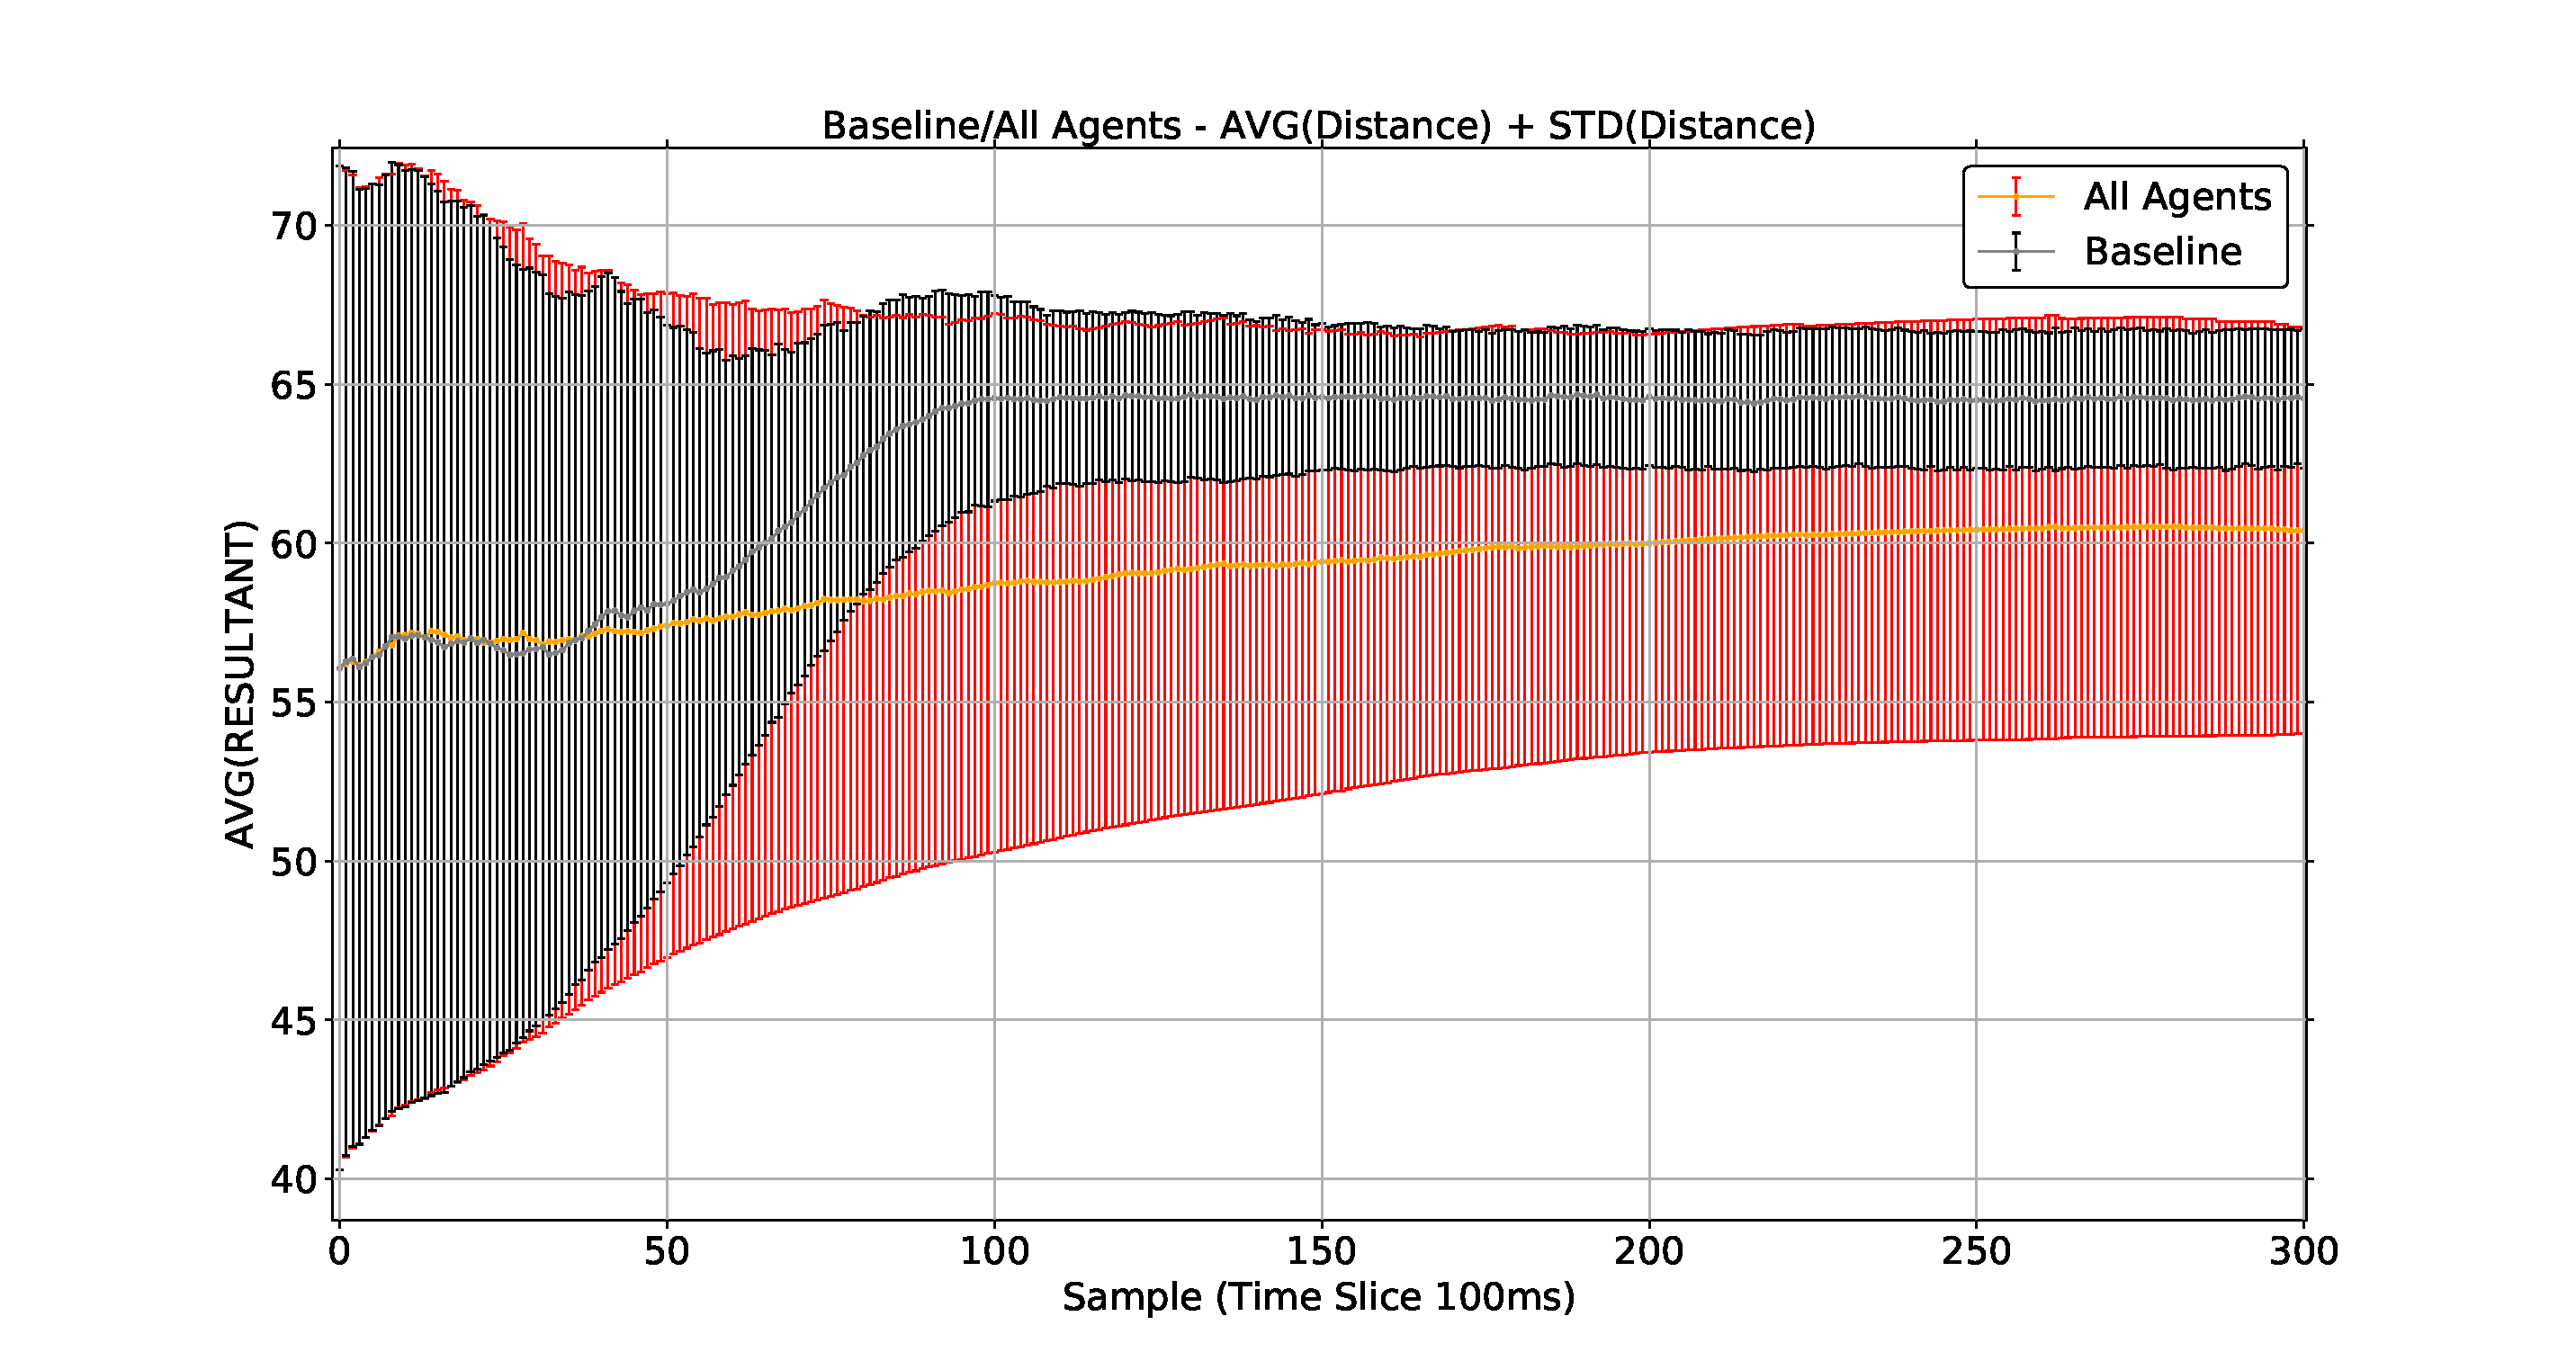
\includegraphics[width=14cm]{CHAPTER-6/figures/BaselineAllAgentsDist1}
\end{center}
\caption{Baseline/All agents comparison (distance)\label{reduced:BaselineAllAgentsDist1}}
\end{figure}

Figure~\ref{reduced:BaselineAllAgentsDist1} shows the effect on the inter-agent distances. The average distance is lower than the baseline. This effect is caused by the \textit{direction vector} reducing the effect of the repulsion field. The agents therefore compress slightly due to the cohesion.

A curious effect of having all the GPS sensors enabled is that as the swarm approaches the destination there is an increased compression effect and the internal disturbance increases. This is the result of the agents `pulling' in a cone effect. The agents paths converge on the destination~(Figure~\ref{reduced:ConicalPath}). This effect is caused by the number of agents being effected by a \textit{direction vector}. This effect is less identifiable if a swarm's target is at a greater distance.  

\begin{figure}[H]
\begin{center}
\includegraphics[width=8cm]{CHAPTER-6/figures/ConicalPath}
\end{center}
\caption{Conical destination trajectories\label{reduced:ConicalPath}}
\end{figure}

This effect can be seen in both the magnitudes shown in~Figure~\ref{reduced:BaselineAllAgentsMag2} and in the distances shown in~Figure~\ref{reduced:BaselineAllAgentsDist2} which both show the averages initially decreasing but then increasing again as the swarm approaches the destination. This is accompanied by a greater standard deviation caused by the \textit{direction vector} affecting the priority of the swarm as agents are drawn to the destination reducing the effect of the \textit{inter-agent vectors} creating stable structures.
%BASELINE-ALLAGENTS-MAG.py
\begin{figure}[H]
\begin{center}
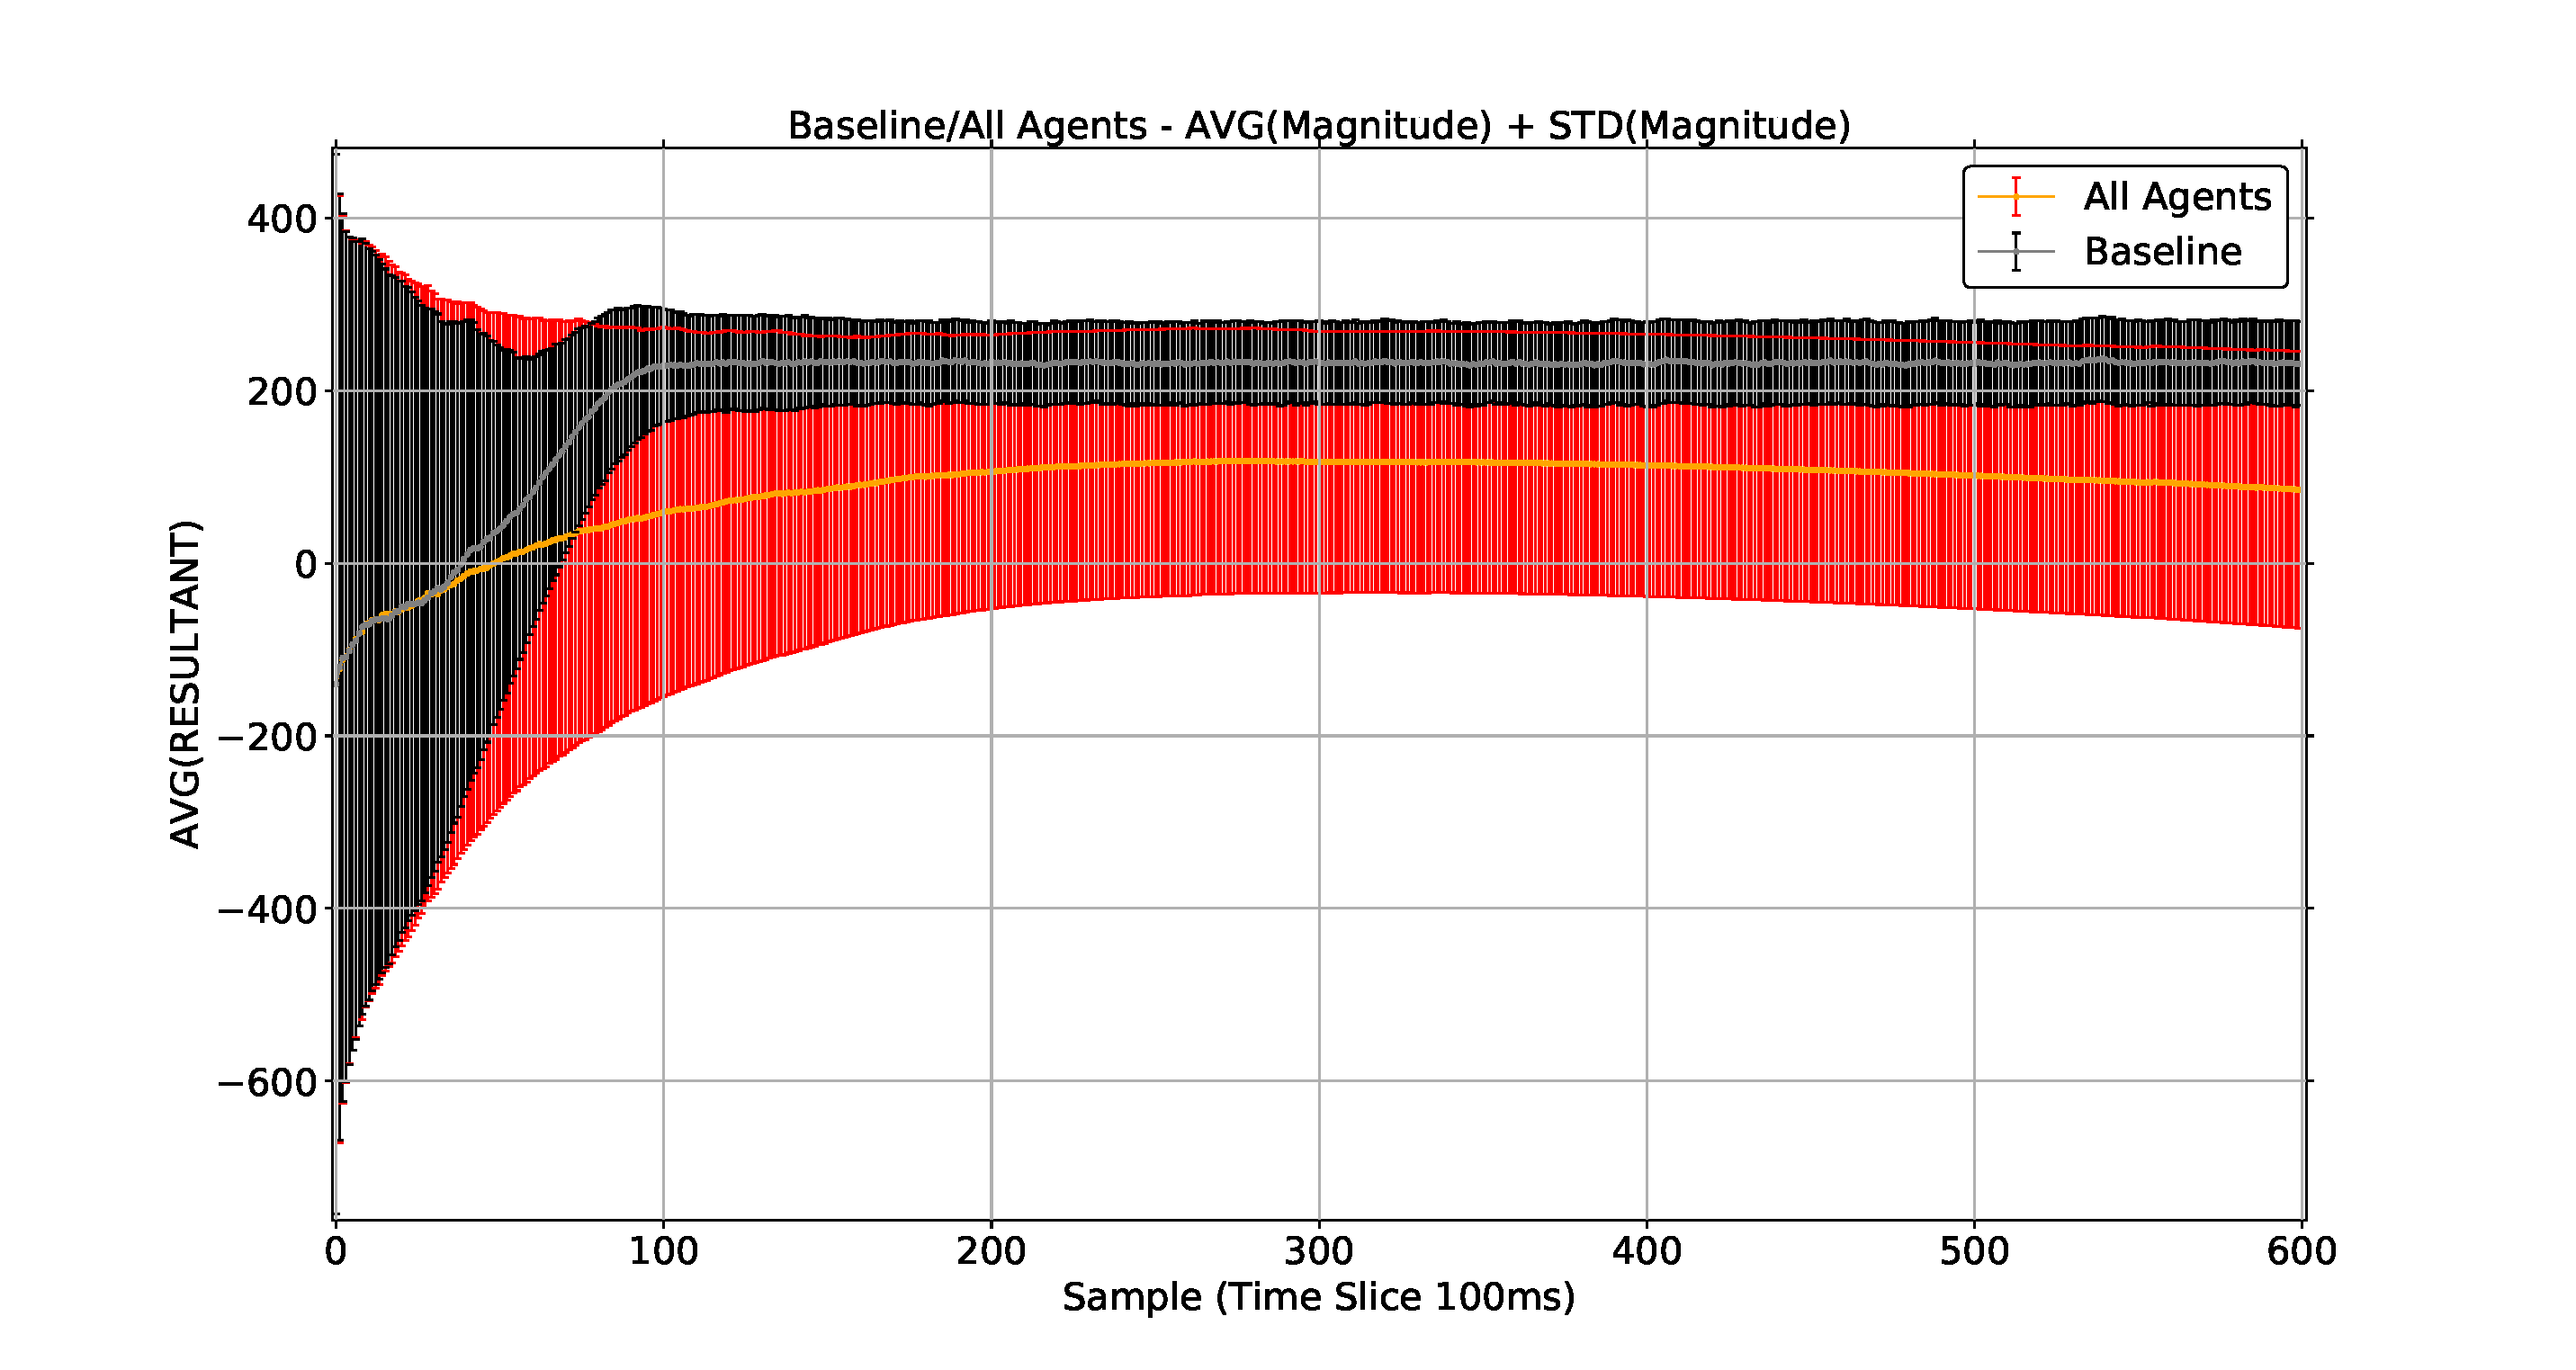
\includegraphics[width=14cm]{CHAPTER-6/figures/BaselineAllAgentsMag2}
\end{center}
\caption[Baseline/All agents magnitude comparison]{Baseline/All agents \textit{inter-agent vector} magnitude comparison (60 seconds)\label{reduced:BaselineAllAgentsMag2}}
\end{figure}
%BASELINE-ALLAGENTS-DIST.py
\begin{figure}[H]
\begin{center}
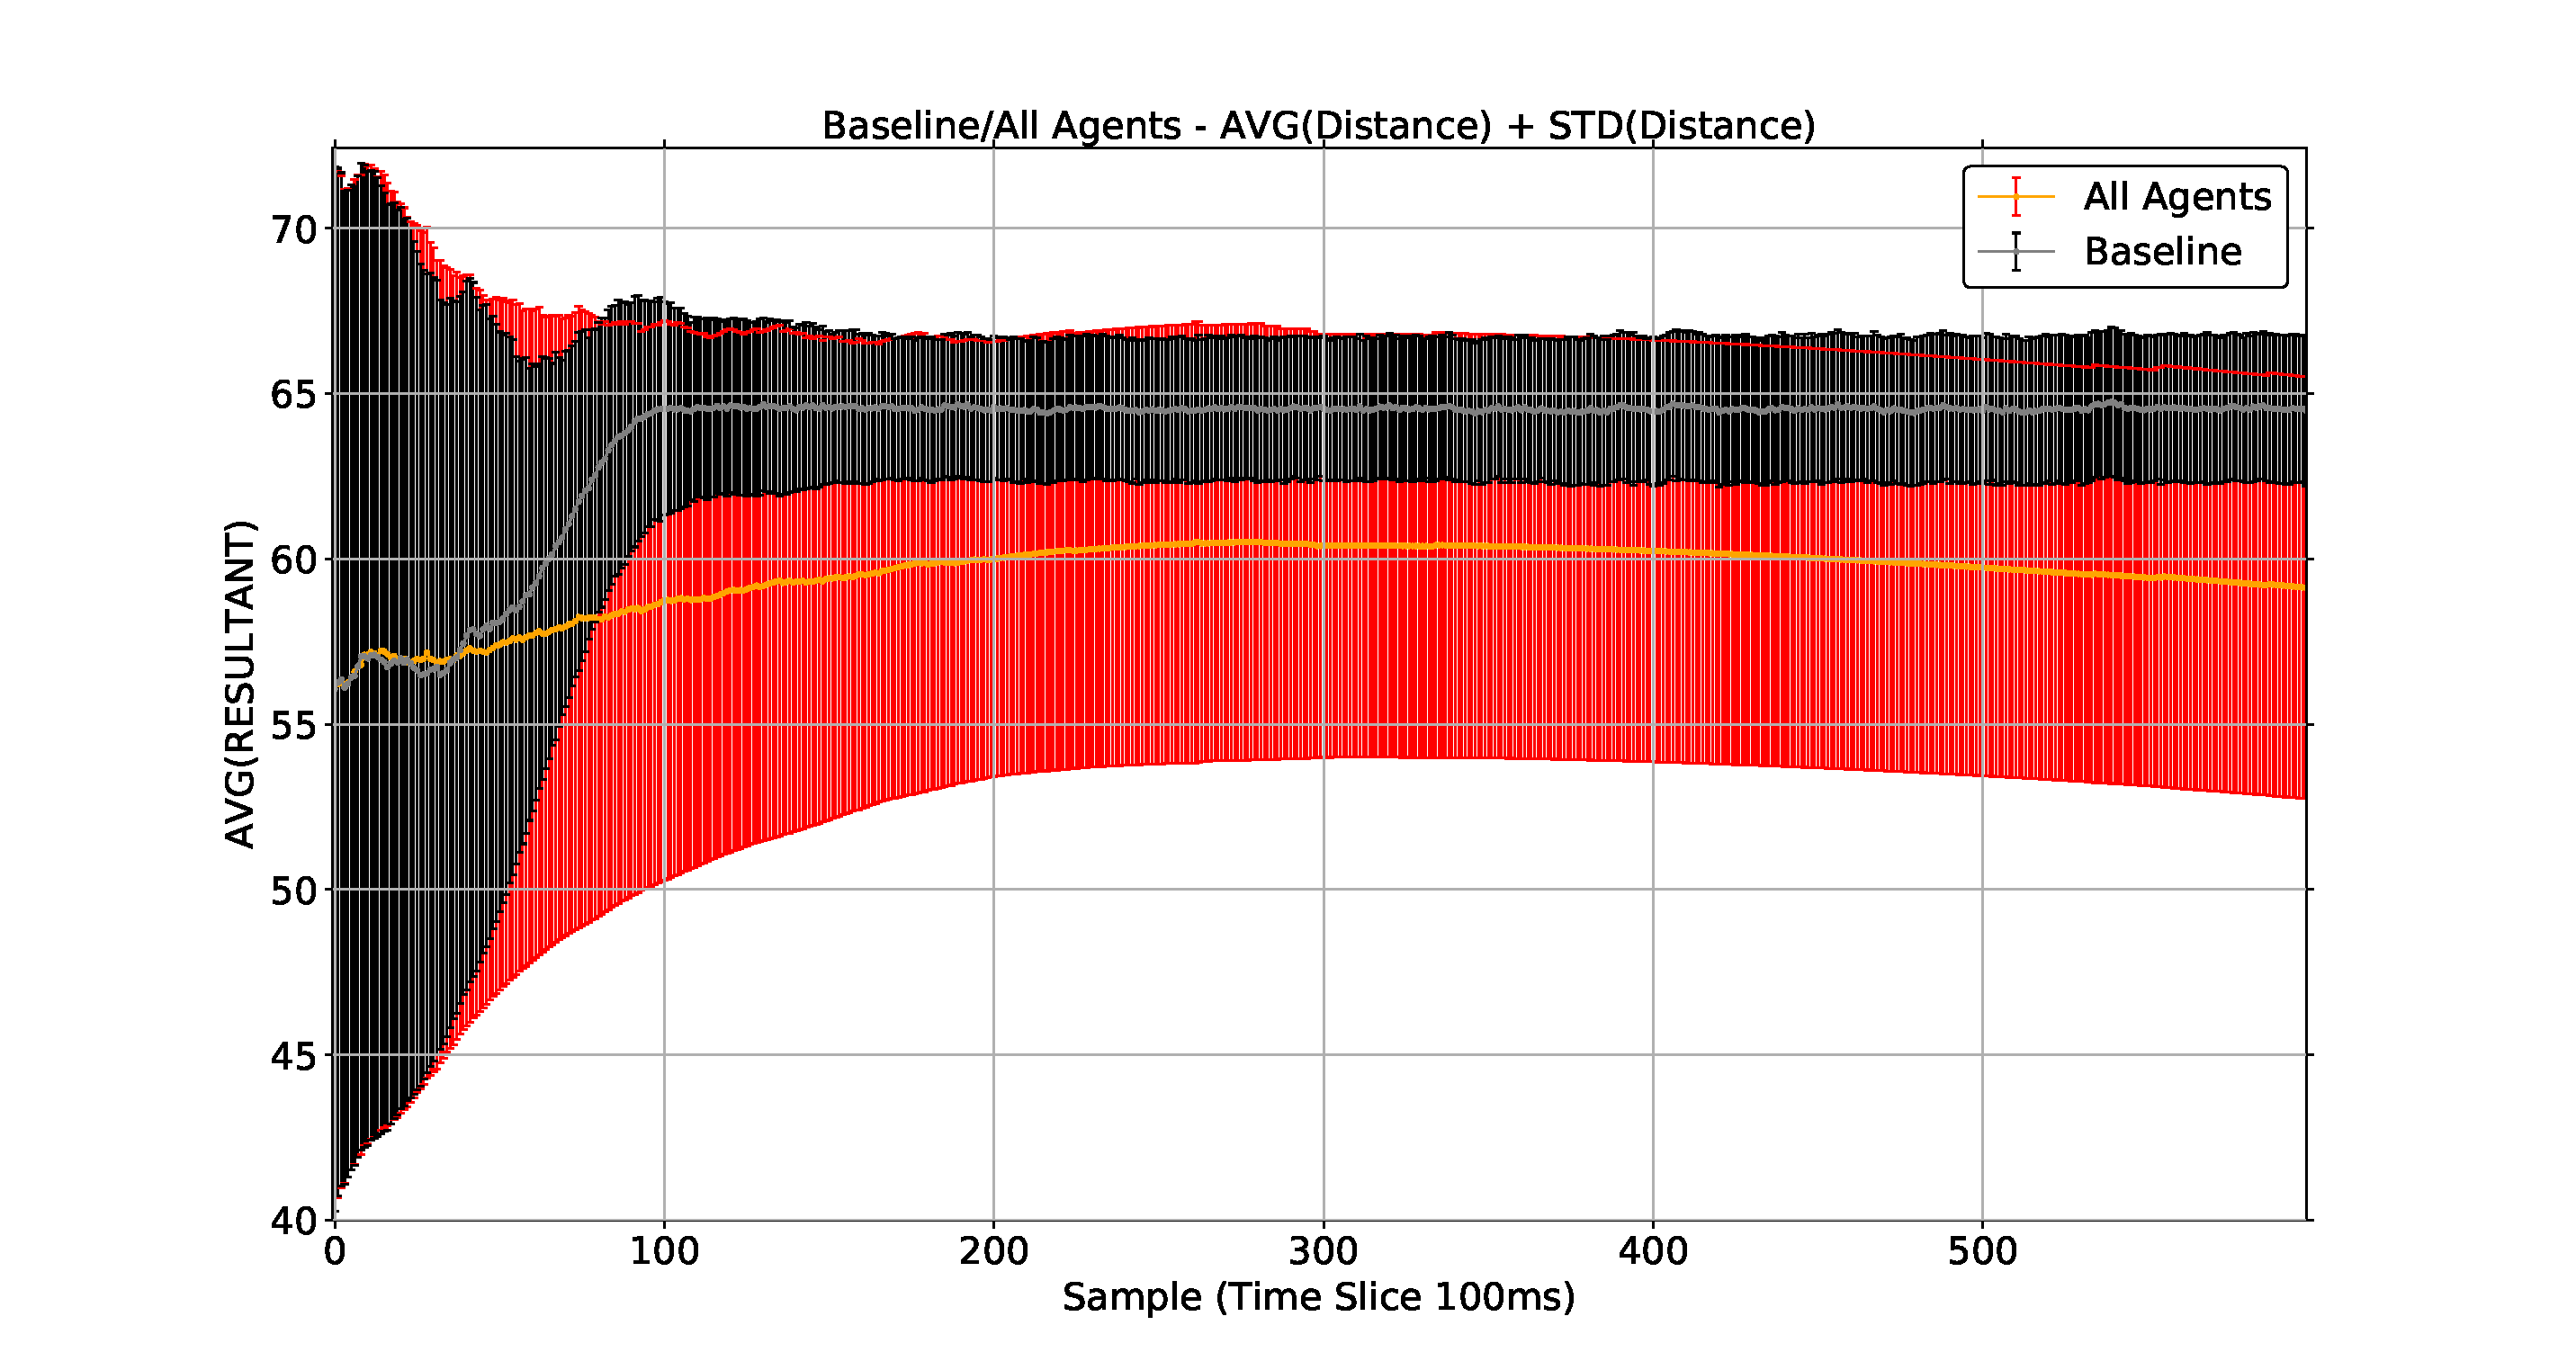
\includegraphics[width=14cm]{CHAPTER-6/figures/BaselineAllAgentsDist2}
\end{center}
\caption{Baseline/All agents distance comparison (60 seconds)\label{reduced:BaselineAllAgentsDist2}}
\end{figure}

\section{Simple multifaceted swarm (basic-count)} 
In a simple multifaceted swarm the propagation towards the goal is achieved by generating a \textit{destination vector} for an agent when the agent conforms to a simple counting rule. This \textit{destination vector} is obtained by using the agent's GPS to identify its current coordinate and generating a vector from that coordinate to a specific destination point. This rule creates a subset of agents that apply a local \textit{direction vector} to their movement. This has the effect of creating a directional effect on the whole swarm. The aggregate \textit{direction vector} magnitude of the swarm is less than that produced when all agents apply a \textit{direction vector}. This reduction is further diluted by agents without the \textit{direction vector} calculating a \textit{movement vector} to an equilibrium position~(Equation~\ref{eq:BotDirection1}). This change in the aggregate \textit{direction vector} will impact on a swarm's `jitter'. This is discussed in more detail in~\autoref{sec:AlternateBias1}. With there only being a limited number of peripheral agents invoking their GPS signal there will also be a net reduction in the energy usage of the swarm~(\autoref{reduced:EnergyReductionGPS}).

A swarm with the appropriate field effects will propagate towards hexagons made from a central agent and six neighbours~(Figure~\ref{fig:StableForms}). A swarm can be influenced by its surroundings, which involves the interaction of other agents (as neighbours) and obstacles which can cause a compression of the agents. Compression can also occur during the stabilisation phase of a swarm. These situations can cause an agent to have less than 6 neighbours but still be surrounded. A general rule therefore to detect a rudimentary boundary of a hexagonal swarm is to calculate the number of neighbours an agent has. If the total is less than five ($nbr(b) < 5$) then there is a high probability that the agent is either in a void within the swarm or on an external perimeter. If an agent is on a perimeter or a void the it should enable its GPS and become a coordinator and provide a directional bias to the swarm via its \textit{direction vector}. This coordinator role affects the immediate neighbours \textit{movement vector} through cohesion/repulsion~(Figure~\ref{reduced:SimpleMulti12}). This simple detection algorithm allows a directional bias to be induced into a swarm with minimal computational impact on the coordinator agents. The issue of voids and perimeters is discussed in~section~\ref{sec:complexMulti} and chapter~\ref{chapter:ConcaveReduction}.

\subsection{Simple multifaceted algorithm}
The mechanism to enable a coordinator agent is to count the number of neighbours that an agent has~(Algorithm~\ref{algo:neighbourDetect}). This process is already part of the cohesion and repulsion calculations.

\begin{algorithm}[H]
\DontPrintSemicolon
\SetAlgoLined
\KwData{$b,S$}
\tcc{$b$ is an agent and $S$ is a set of agents}
\tcc{The set of agent could be provided by an omni directional camera or a set of ultrasonic sensors}
$N \longleftarrow \emptyset$\;
\ForEach(\tcc*[h]{$b^{'}$ is each agent in $S$}){$b^{'}$ in $S$}
{
  \If(\tcc*[h]{$D_b$ is the neighbour range}){$length(bb') < D_{b}$}
  {
     $N \longleftarrow N \cup \{b\}$
  }
}
\tcc{$N$ is a set of Bots $b_1,b_2,\ldots,b_n$}
\KwRet{$N$}
\caption[Neighbour Detection]{nbr(b)}\label{algo:neighbourDetect}
\end{algorithm}

\subsection{Basic-count effect\label{section:compareBaselineBasicCount1}}
Figures~\ref{reduced:BaselineBasicCountMag1} and \ref{reduced:BaselineBasicCountDist1} show the comparison of the baseline swarm against the goal-based swarm with reduced GPS usage. Both graphs show that the settling period of the swarm from the disorganised state is very much in line with the settling period of the baseline swarm. This is due to the algorithm's effect when the swarm is initially compressed. The neighbour count prevents any agents from being coordinators ($|nbr(b)| > 5$). This is supported by the propagation of the coordinator role in figure~\ref{fig:SwarmNeighbourCount}. The swarm therefore acts in a similar manner to the baseline. As the simulation progresses the swarm settles into a condition that is similar to baseline with a higher deviation and lower mean resultant \textit{inter-agent vector}. This is due to there being a \textit{direction vector} which impacts on the coordinator agents and propagates to the non-coordinator agents through proximity. This effect is shown in figure~\ref{metric:StabilityNullVector}. 

\begin{figure}[H]
\begin{center}
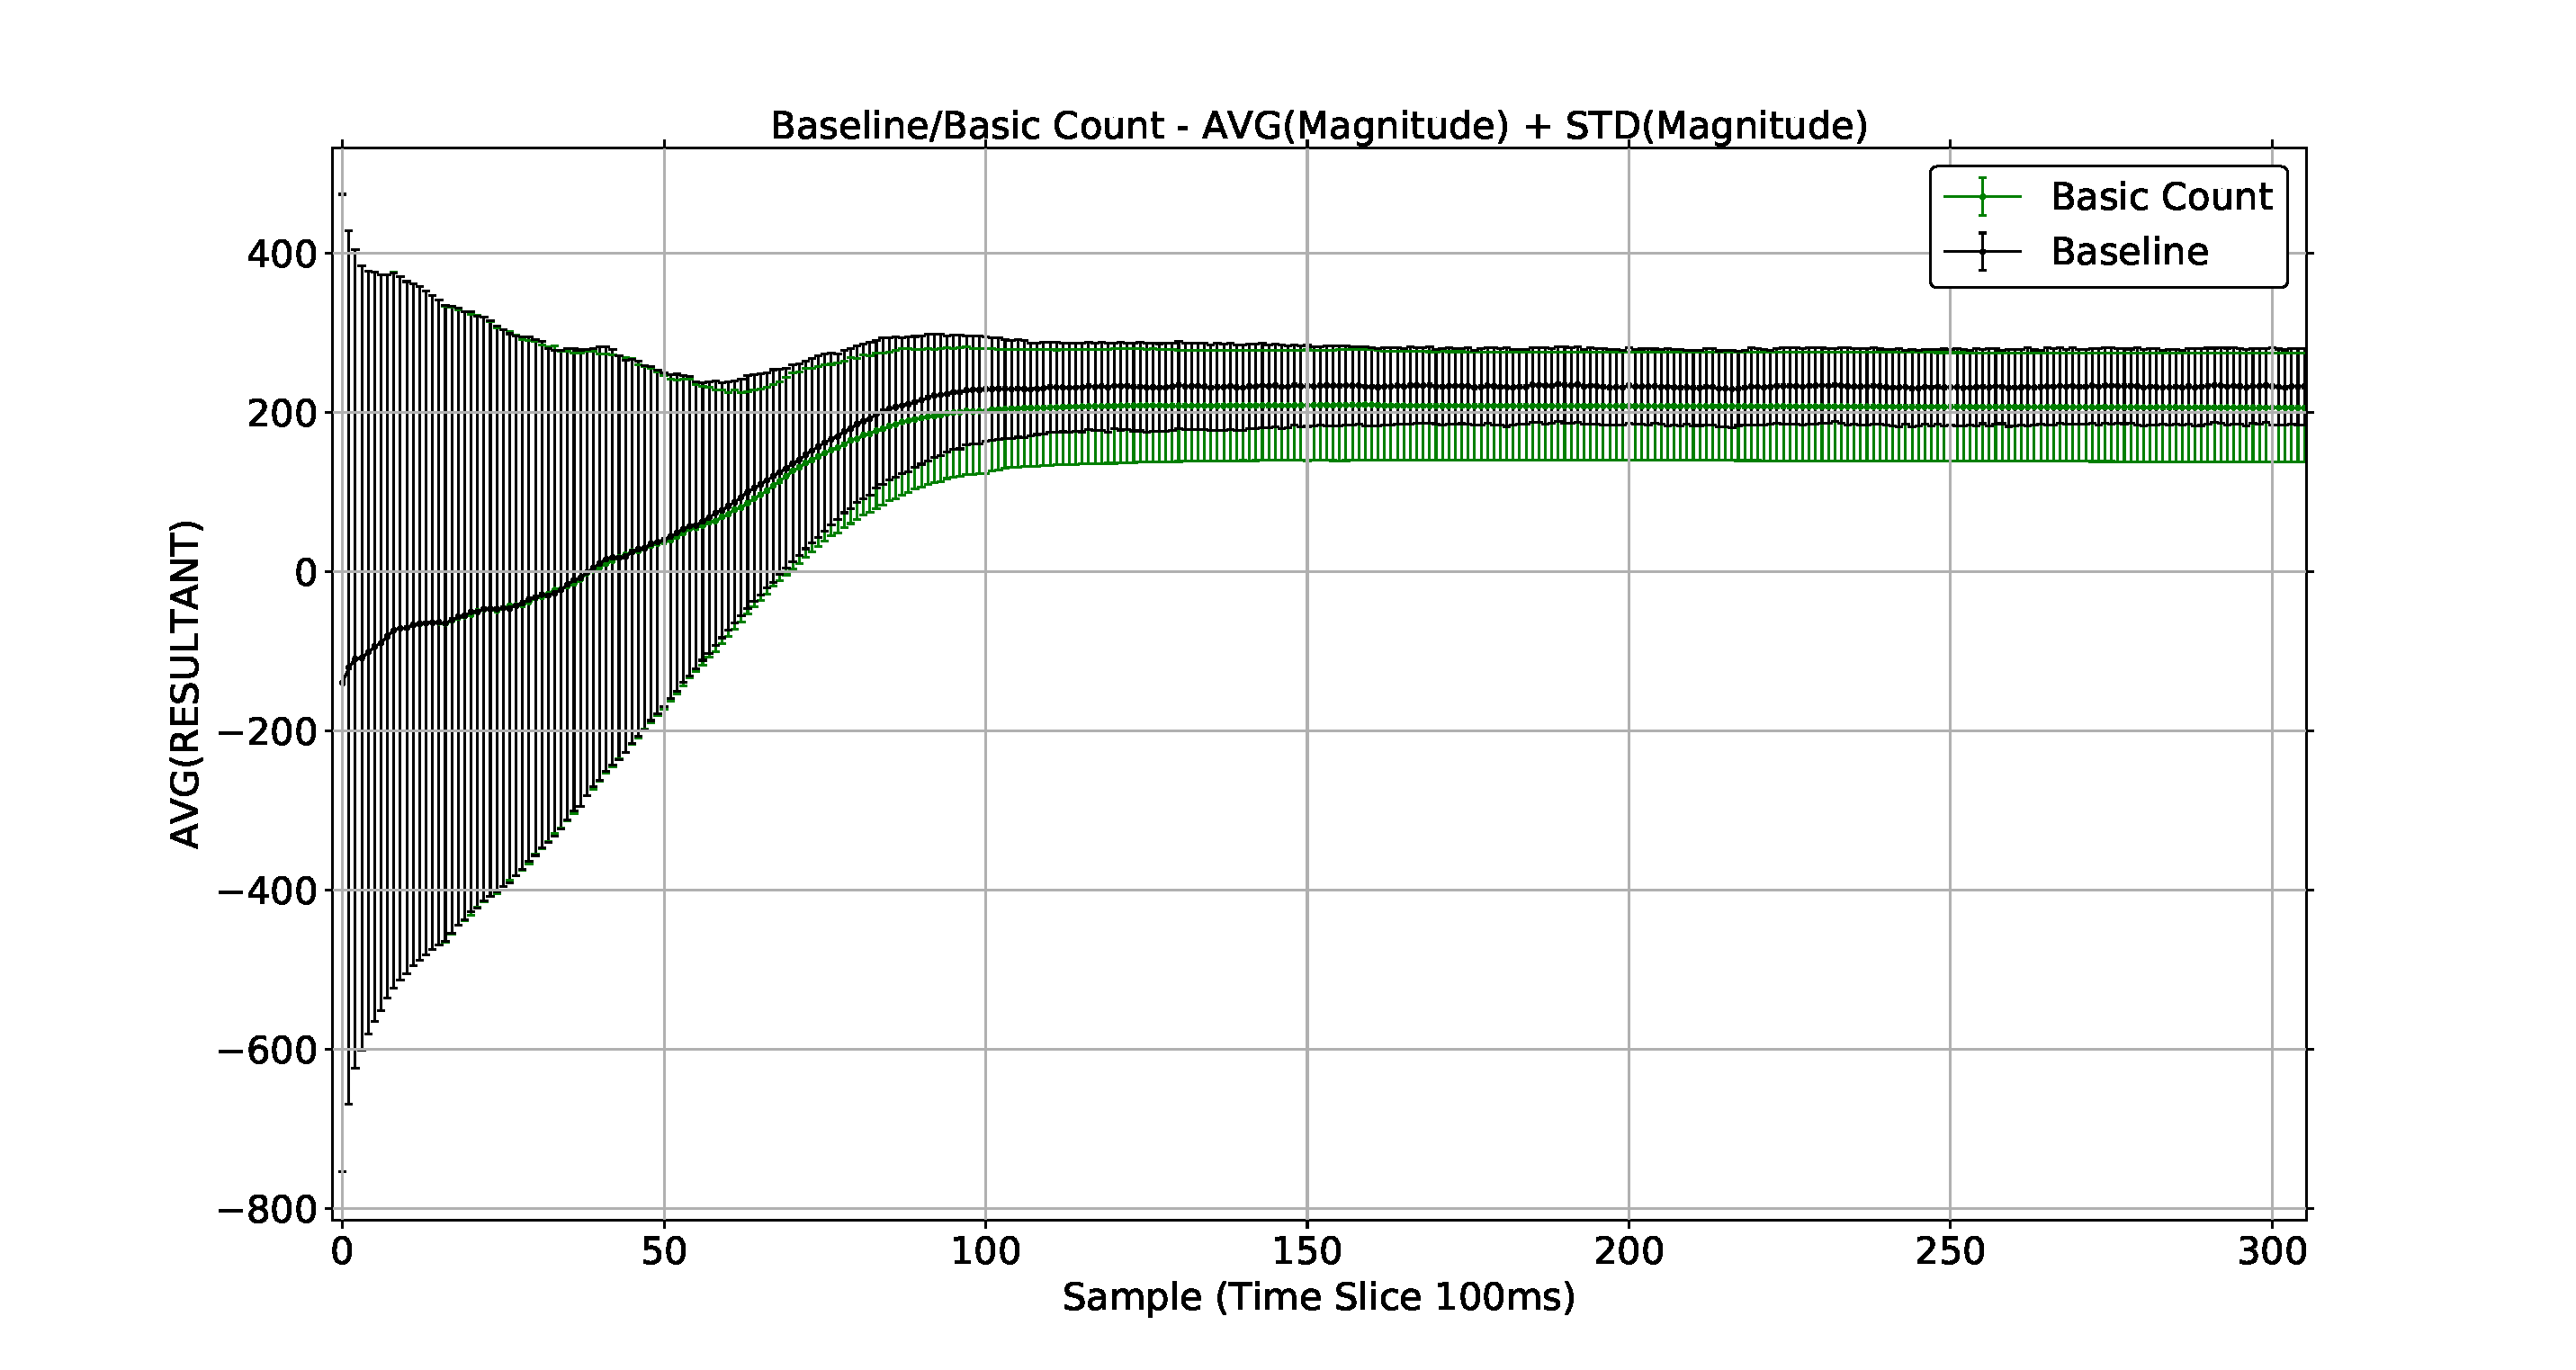
\includegraphics[width=14cm]{CHAPTER-6/figures/BaselineBasicCountMag1}
\end{center}
\caption{Baseline/basic-count magnitude potential comparison\label{reduced:BaselineBasicCountMag1}}
\end{figure}

Figure~\ref{reduced:BaselineBasicCountMag1} shows that initially the average \textit{inter-agent vector magnitude} can be seen to follow the same trend as the baseline. This is expected as the algorithm's selection criteria is such that no GPS sensors are enabled when the swarm is compressed and the agents will have a neighbour count well above the trigger level for the coordinator role. When the swarm expands sufficiently the trigger level is met by some agents and there is a gradual increase in the number of coordinators. This also creates a greater distribution of resultant \textit{interaction vectors}, shown as the change in the standard deviation. 

\begin{figure}[H]
\begin{center}
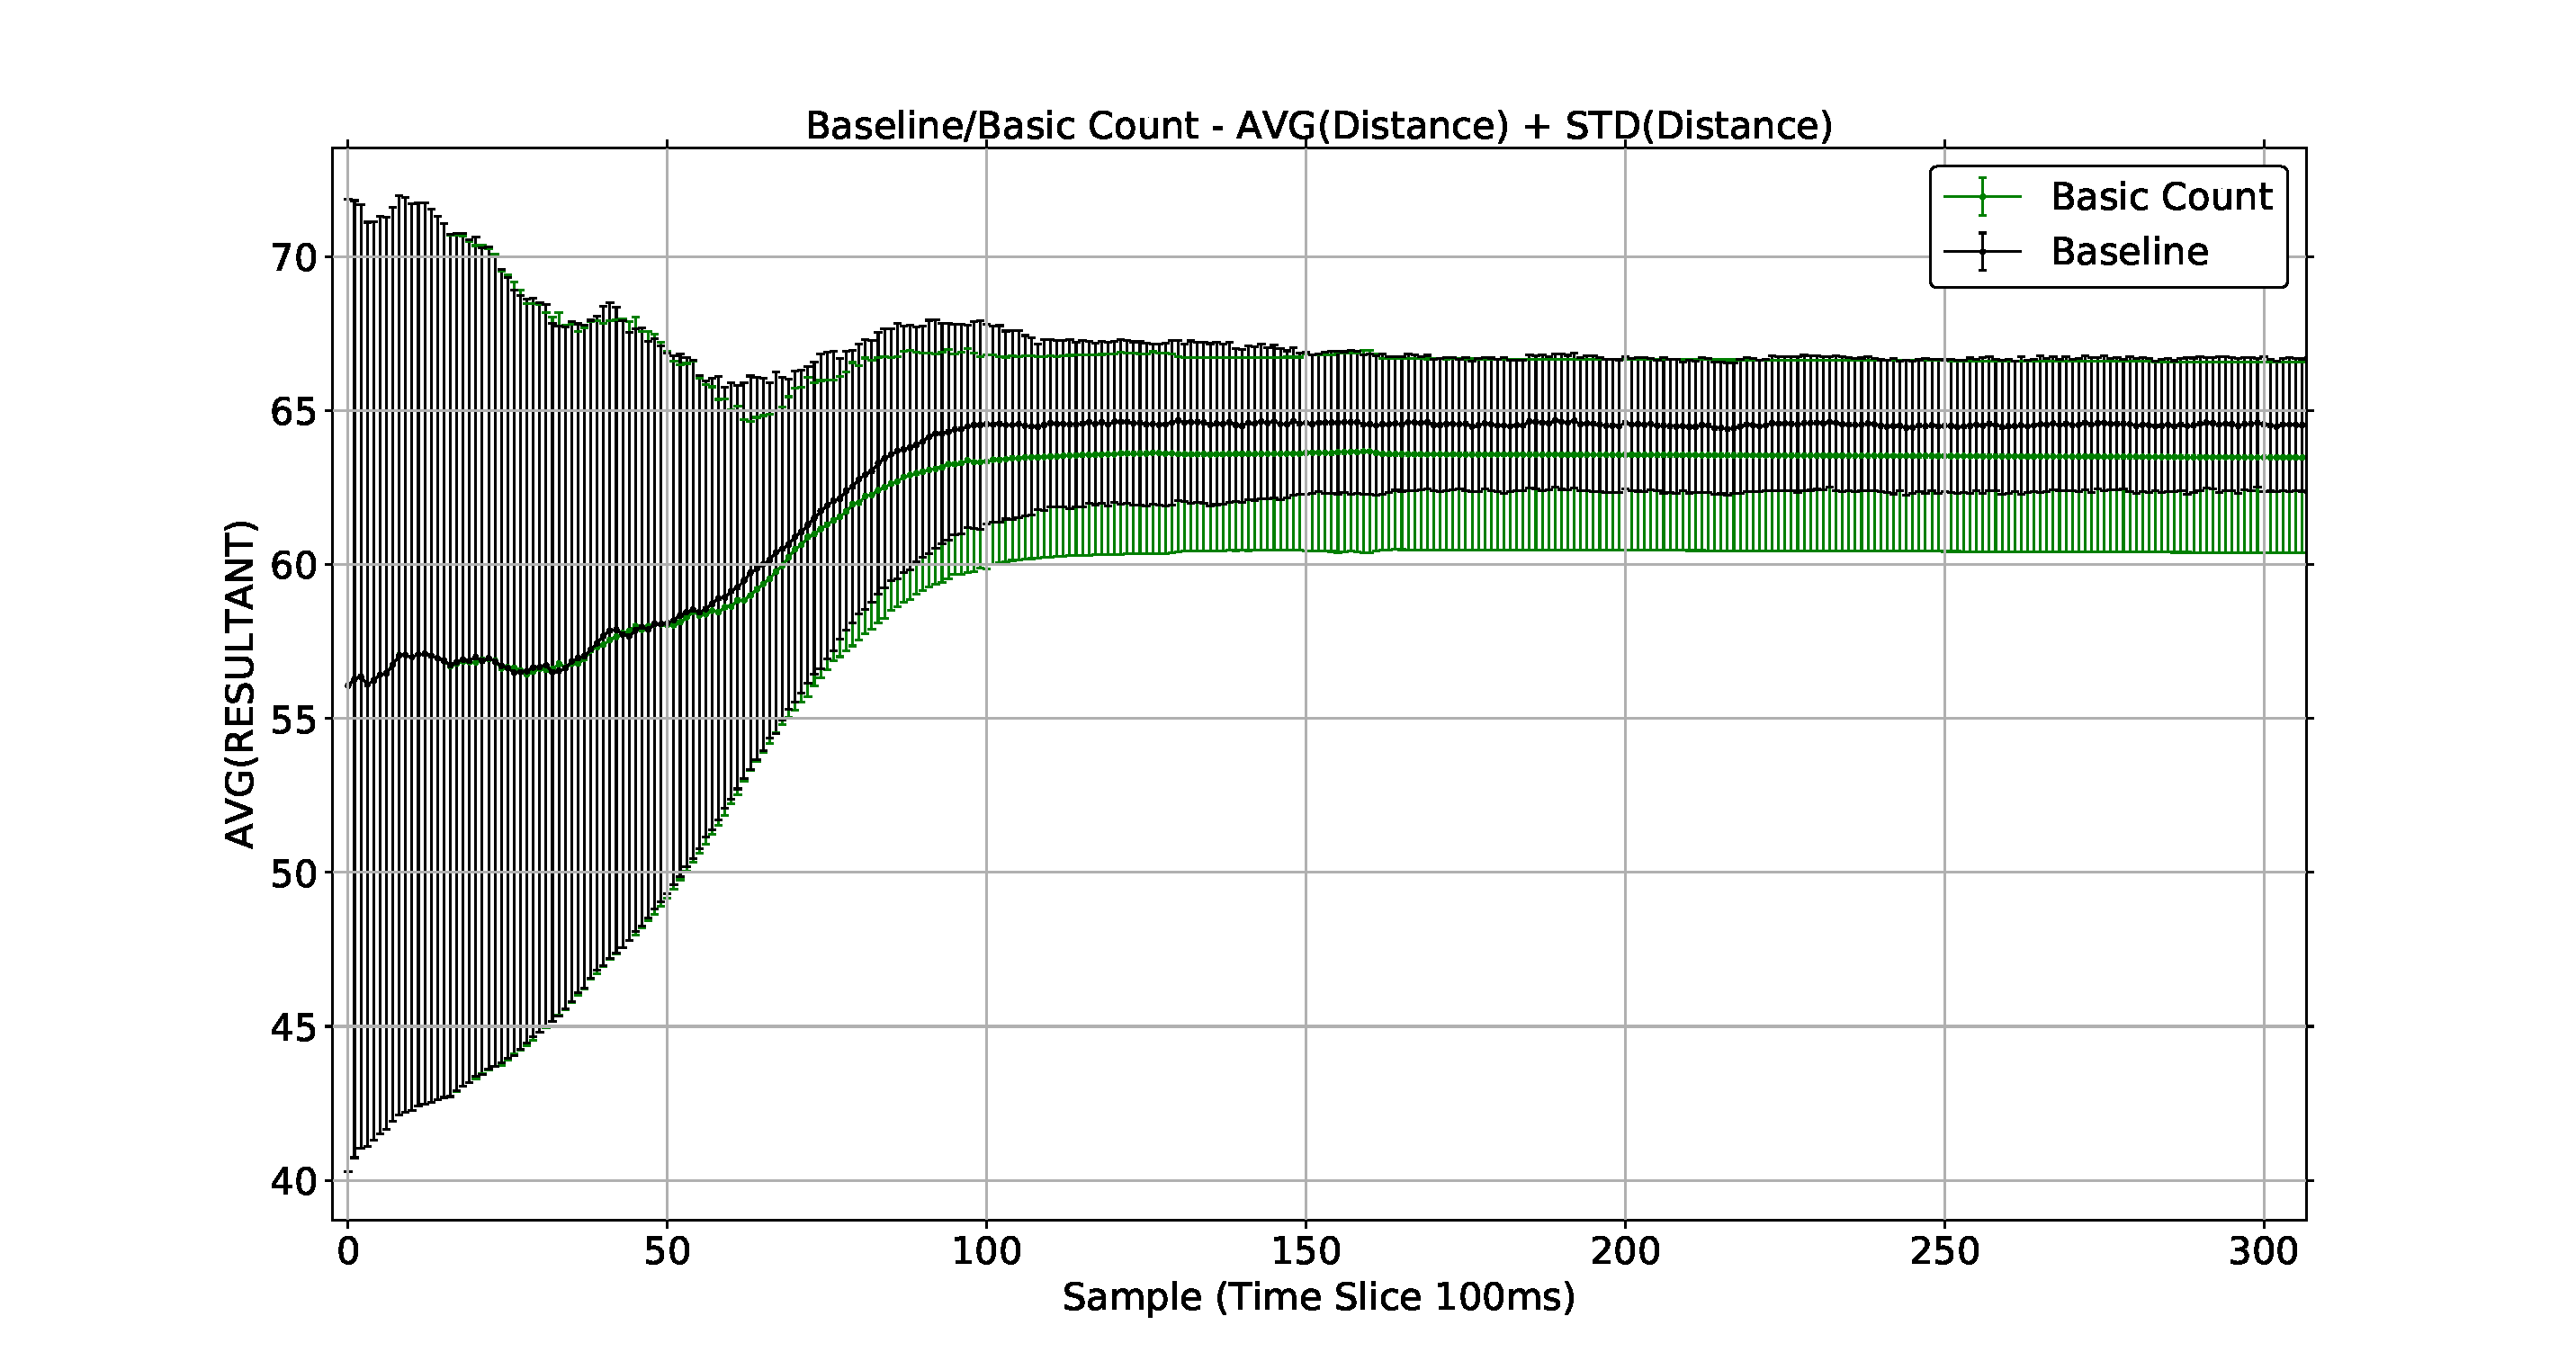
\includegraphics[width=14cm]{CHAPTER-6/figures/BaselineBasicCountDist1}
\end{center}
\caption{Baseline and basic-count distance comparison\label{reduced:BaselineBasicCountDist1}}
\end{figure}
 
Figure~\ref{reduced:BaselineBasicCountDist1} shows that the impact of the directional bias allows the agents to move closer together. This increased closeness reduces the effective area coverage of the swarm. 

Figure~\ref{reduced:SimpleMulti12} shows a screen shot of the simulator using the basic-count algorithm. The reduction in GPS usage is limited to edge based agents of the swarm. Some perimeter agents are not identified as a coordinator due to the number of neighbours they have being $\geq5$. These agents tend to be indented on a perimeter edge. This feature will be discussed in more detail in chapter~\ref{chapter:ConcaveReduction}.

\begin{figure}[H]
\begin{center}
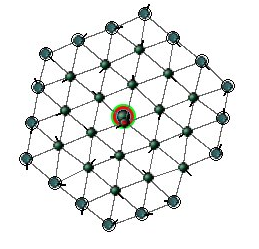
\includegraphics[width=7cm]{CHAPTER-6/figures/SimpleMulti2}
\end{center}
\caption[Simple multifaceted agents]{Simple multifaceted agents (\textit{screen shot from simulator})\label{reduced:SimpleMulti12}}
\end{figure}

\section{Complex multifaceted swarm (full-perimeter)}\label{sec:complexMulti} 
A complex multifaceted swarm is based upon the full detection of perimeters in a swarm. There are two perimeters that can be detected, convex and concave~\cite{MD:09,MJ:08}. Convex perimeters enclose agents and concave perimeters create voids. Figures~\ref{concave:VoidPerimeter1} and \ref{concave:VoidPerimeter2} show these two perimeter types. The concave perimeter is highlighted in red and the convex perimeter is highlighted in green

\begin{figure}[H]
\centering
\subfigure[Void and perimeter]{
	 \includegraphics[width=4cm]{CHAPTER-6/figures/PerimeterBots1}
    \label{concave:VoidPerimeter1}
}
\subfigure[Multiple perimeters]{
	 \includegraphics[width=6.5cm]{CHAPTER-6/figures/PerimeterBots2}
    \label{concave:VoidPerimeter2}
}
\caption{Swarm perimeters and voids}
\label{fig:SwarmVoids}
\end{figure}

There is an exceptional circumstance that must be considered in perimeter detection. This is covered in \autoref{section:PerimeterErrorLocalisation}. Figure~\ref{fig:FullPerimeter1} is a screen shot from the simulator showing both perimeter types detected. The algorithm does not distinguished between the types. 

\begin{figure}[H]
\begin{center}
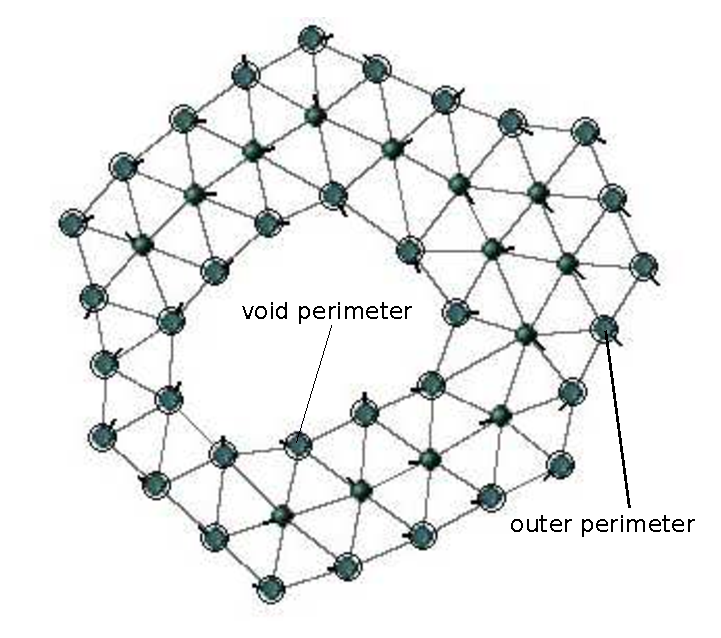
\includegraphics[width=7cm]{CHAPTER-6/figures/FullPerimeter}
\end{center}
\caption[Swarm with full perimeter detection]{Swarm with full perimeter detection (\textit{screen shot from simulator})\label{fig:FullPerimeter1}}
\end{figure}

The full-perimeter algorithm allows a predictable subset of agents to be identified. This subset can be used to influence the overall direction of the swarm. The full-perimeter detection algorithm detects similar agents to the basic-count algorithm but also identifies `indented' agents that the basic-count algorithm ignores. The basic-count algorithm identifies these agents as having a neighbour count beyond the threshold. These additionally detected agents are used in void reduction which is discussed in chapter~\ref{chapter:ConcaveReduction}.

\subsection{Full-perimeter coordinator detection}\label{sec:PerimeterAgentDetection} 
The process of detecting a perimeter agent is based upon identifying when the agent in not surrounded by interconnected neighbours~(\autoref{reduced:Perimeter1}). The process has several conditional checks that detect the status of an agent, each step is discussed below. 

\begin{figure}[H]
\begin{center}
\includegraphics[width=6cm]{CHAPTER-6/figures/Perimeter1}
\end{center}
\caption{Complex multifaceted agents \label{reduced:Perimeter1}}
\end{figure}

The first check is a short circuit count of the number of neighbours. This is the same process used to the basic-count algorithm. If an agent has $\leq 4$ neighbours and the swarm parameters are for a hexagonal swarm configuration then the agent is a perimeter agent and therefore a coordinator. This identification process is shown in~figure~\ref{SmallNeighbourCount}. 

\begin{algorithm}[H]
\DontPrintSemicolon
\SetAlgoLined
\KwData{$b$}
\tcc{for $nbr()$ see Equation~\ref{eq:Neighbours1} on page \pageref{eq:Neighbours1}}
\If{$\card{nbr(b)} \leq 4$}{
   \KwRet{True}\;
}
\KwRet{False}\;
\caption{SmallNeighbourCount}\label{SmallNeighbourCount}
\end{algorithm}

If the short circuit neighbour count check fails then further conditions must be checked. The additional checks require a dictionary of agent/angular values to be generated~(Equation~\ref{eq:ConcaveVoidPhysics1}). Algorithm~\ref{algo:getNeighbourAngles} shows how the dictionary of agent/angle values are produced.   

\begin{center}
\begin{equation}‎
\label{eq:ConcaveVoidPhysics1}
S_b \buildrel \Delta \over =‎ \{(b',\angle\{(b'~b~b^0)) : b' \in nbr(b)\}
\end{equation}‎
\end{center}

Equation~\ref{eq:ConcaveVoidPhysics1} generates the dictionary set of all the neighbours along with an angle that each of the agent's neighbour's make with the first detected neighbour.
%% 
%% \begin{center}
%% \begin{equation}‎
%% \label{eq:ConcaveVoidPhysics2}
%% G_b \buildrel \Delta \over =‎ gap(S_b,\angle<180^\circ)
%% \end{equation}‎
%% \end{center}

Algorithm \ref{algo:getNeighbourAngles} shows the logic to produce the sorted neighbour/angle dictionary. $sort(.)$ sorts the dictionary set generated in~equation~\ref{eq:ConcaveVoidPhysics1} by ascending angle to produce a dictionary of neighbour agents with their relative angle to the first detected neighbour as shown in~equation~\ref{reduced:Perimeter1}.

\begin{algorithm}[H]
\DontPrintSemicolon
\SetAlgoLined
\caption{NeighbourAngle: Sorted by angle}
\KwData{b}
\tcc{$angles$ is a dictionary of agent/angle}
$angles \leftarrow \emptyset$\;
\For{$b^{'}\in b.neighbours$}{
	\eIf{$b.neighbours[0] == b^{'}$}{
      $angles[b^{'}] = 0$\;
	}{
		$newAngle = b.getAngle(b.neighbours[0], b^{'})$\;
	   $angles[b^{'}] = newAngle$\;
	}
}
\KwRet{$sort(angles)$} 
\label{algo:getNeighbourAngles}
\end{algorithm}

Using the angular dictionary from algorithm~\ref{algo:getNeighbourAngles} it is possible to identify if adjacent neighbours can detect each other. If the agent is within all of its neighbours boundary then it is not on the perimeter~(Algorithm~\ref{algo:checkVisibility}). 

As the agents are monolithic all agents have the same field effects the `visibility' of two neighbours can be determined. The angle and distance of each neighbour pair and the angle they create allows cosine rule to be used to calculate the distance the neighbours are apart as shown in~Equations~\ref{eq:CosineRule1} and~\ref{reduced:Triangulate}. The distance is then checked against the neighbour range field effect. If the distance is $\leq N_b$ where $N_b$ is the \textit{neighbour field} then the agent can assume the neighbours have `sight' of each other. 

\begin{figure}[H]
\begin{center}
\includegraphics[width=4.5cm]{CHAPTER-6/figures/Triangulate}
\end{center}
\caption{Neighbour visibility\label{reduced:Triangulate}}
\end{figure}

\begin{equation}\label{eq:CosineRule1}
z = \sqrt{x^2 + y^2 - 2xy~\cos(\theta)}
\end{equation}‎

The full visibility check~(Algorithm~\ref{algo:checkVisibility}) takes each pair in turn and using the cosine rule~(Equation~\ref{eq:CosineRule1}) checks for a `visibility gap'. 

\begin{algorithm}[H]
\DontPrintSemicolon
\SetAlgoLined
\caption{CheckVisibility}
\KwData{b,angles}
\For{$i \leftarrow 0$ \KwTo $size(angles)-1$}{
	\eIf{i == size(angles)-1}{
		\If{$cosrule(b,angles[size(angles)-1][0],angles[i][0]$}{
   		\KwRet{True}
   	}
	}
	{\If{$cosrule(b,angles[i + 1][0],angles[i][0]$}{
			\KwRet{True}
		}
	}
}
\KwRet{False}
\label{algo:checkVisibility}
\end{algorithm}

There is one exception to the neighbour visibility check. Due to compression of the swarm, which can be caused by an initial deployment configuration~(Figure~\ref{fig:SampleSwarm200-1} page \pageref{fig:SampleSwarm200-1}) or when an obstacle is in the path of the swarm, the agent's neighbours are able to `see' other neighbours but a pair of sequential neighbours could create an angle $> 180^\circ$ as shown in~Figure~\ref{reduced:Perimeter2}. In this case the agent is on the outside of the enclosed neighbour space, the agent is therefore on a perimeter. 

\begin{figure}[H]
\begin{center}
\includegraphics[width=5.5cm]{CHAPTER-6/figures/Perimeter2}
\end{center}
\caption{Convex multifaceted agents \label{reduced:Perimeter2}}
\end{figure}

This phenomenon requires the detection process to identify the angles that all the agents create from an arbitrary point, in this case the first identified neighbour. The neighbours must then be checked to determine if any neighbour pair create an angle $> 180^\circ$~(Figures~\ref{reduced:Perimeter1}~Algorithm~\ref{algo:checkConvex}). This process includes a short circuit in that as soon as a gap is found the check terminates. 

\begin{algorithm}[H]
\DontPrintSemicolon
\SetAlgoLined
\caption{CheckConvex}
\KwData{angles}
\For{$i \leftarrow 0$ \KwTo $size(angles)-1$}{
	\eIf{i == size(angles)-1}{
		\If{$360 - angles[loop][1] \geq 180$}{
   		\KwRet{True}
   	}
	}{
		\If{$angles[loop + 1][1] - angles[loop][1] \geq 180$}{
			\KwRet{True}
		}
	}
}
\KwRet{False}
\label{algo:checkConvex}
\end{algorithm}

The complete perimeter detection algorithm using this `cyclic-angular-neighbour-check' methodology is show in~algorithm~\ref{algo:checkPerimeter}. The first part of the algorithm is the short circuit check~(\textit{SmallNeighbourCount(b)}). This is only followed by the visibility check (\textit{CheckVisibility(b,angles)}) if the short circuit fails. If the visibility check is confirmed, which is another short circuit method, the convex check is carried out~(CheckConvex(angles)). This sequence ensures the minimum computational overhead for the agent check. 

\begin{algorithm}[H]
\DontPrintSemicolon
\SetAlgoLined
\caption{CheckPerimeter}
\KwData{$b,S$}
\If{SmallNeighbourCount(b,S)}{
	\KwRet{True}
}
$angles = NeighbourAngle(b)$\;
\If{CheckVisibility(b,angles)}{
	\If{CheckConvex(angles)}{
		\KwRet{True}
	}
}
\KwRet{False}
\label{algo:checkPerimeter}
\end{algorithm}

\subsubsection{Perimeter detection errors\label{section:PerimeterErrorLocalisation}}
With the proximity of the agents needing to be hexagonally connected and the requirement to eliminate inter-agent communications to allow for arbitrary sized swarms, there is the possibility of a localised perimeter detection algorithm error. When a swarm is compressed a localised anomaly can arise where agents are in a hyper-connected structure on a perimeter. When this anomaly occurs the proposed algorithm will produce a false positive result for the affected agents. 

\begin{figure}[H]
\begin{center}
\includegraphics[width=5cm]{CHAPTER-6/figures/PerimeterError1}
\end{center}
\caption{Perimeter detection error\label{reduced:CompressedRangeError}}
\end{figure}

Figure~\ref{reduced:CompressedRangeError} shows two agents $b^{'}$ and $b^{''}$. The agents have visibility of each other as shown by the green field effects. The agents can also `see' another agent beyond their immediate neighbour. Agent $b^{'}$ is influenced by $b^{''}$ and neighbour 1. Agent $b^{'}$ is influenced by $b^{''}$ and neighbour 5. Due to these interactions both agents could calculate that they are surrounded by neighbours and are therefore not a part of the perimeter. The visibility issue is indicated by the red lines between $b^{''}$ and 5, and $b^{'}$ and 1. Neighbours 1 and 5 have no visibility of each other. Due to the connectivity shown in red there is a possibility of a failure in full perimeter detection as agents 5 and 1 cannot detect each other. 

The possible pathways that could be detected as the perimeter are: $5 \rightarrow b^{'} \rightarrow 1$, $5 \rightarrow b^{''} \rightarrow 1$. A third alternative of $5 \rightarrow b^{'} \rightarrow b^{''} \rightarrow 1$ could also be used but it is not strictly a true perimeter route as the previous routes are shorter.  

This problem can be resolved fully by introducing a communications channel that would allow the affected agents to negotiate a resolution to chose one of the shorter pathways~\cite{MD:09}, as there is no communications available this is not an option. In this thesis the error is limited to a very specific set of circumstances which will only occur during the initial expansion phase or during obstacle avoidance. The algorithm described in~\autoref{sec:PerimeterAgentDetection} selects both agents as being perimeter agents therefore the problem is resolved by using the pseudo-perimeter ($5 \rightarrow b^{'} \rightarrow b^{''} \rightarrow 1$) ensuring a continuous perimeter is detected. 

The screen shot below shows the algorithm resolving the issue to the pseudo-perimeter in the simulator~(Figure~\ref{reduced:PerimeterAnomaly}).

\begin{figure}[H]
\begin{center}
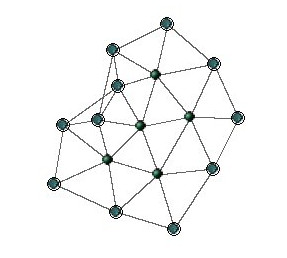
\includegraphics[width=5cm]{CHAPTER-6/figures/PerimeterAnomaly}
\end{center}
\caption{Simulator perimeter detection\label{reduced:PerimeterAnomaly}}
\end{figure}

\subsubsection{Perimeter and void detection}\label{sec:PerimeterVoidDetection} 
The focus of this thesis is the control of arbitrary sized swarms. The identification of the inner and outer perimeters would require a communications mechanism to determine which type of perimeter an agent was a part of~\cite{ZAPS:07,MD:09}. A mean angle $< 180^\circ$ would indicate a void. A mean angle $> 180^\circ$ would indicate an outer perimeter which may be enclose inside a swarm as shown in~figure~\ref{concave:VoidPerimeter2} on page \pageref{concave:VoidPerimeter2}.  

The communications architecture would prevent swarms of an arbitrary size from being coordinated due to the $O(n^{2})$ message propagation time factor~(\autoref{methods:MessagePropogation})~\cite{SHA:07}. It should be noted however that introducing the communications layer would increase the potential functionality of the swarm and may have practical applications in other scenarios where smaller swarms are appropriate. 

A further issue of introducing a communications infrastructure would be the increase in the energy usage of the swarm. Identification of the perimeter type is therefore not practical in context of this thesis.

\subsection{Baseline/full perimeter comparison\label{section:compareBaselineFullPerimeter}}
Figures~\ref{reduced:BaselineFullPerimeterMag1} and \ref{reduced:BaselineFullPerimeterDist1} show the comparisons of the baseline swarm against the goal based swarm using full perimeter detection. 

Figures~\ref{reduced:BaselineFullPerimeterMag1} and \ref{reduced:BaselineFullPerimeterDist1} show that the settling period of the swarm from the disorganised state occurs at a very similar rate to the baseline but the swarm does not settle into a condition that has the same stability as the baseline. This deviation can be expected as the algorithm's selection criteria is such that when the swarm is highly compressed there will be a limited number of perimeter agents effecting the directional bias of the swarm and the majority of internal logic will be the \textit{interaction vectors} expanding the swarm.

\begin{figure}[H]
\begin{center}
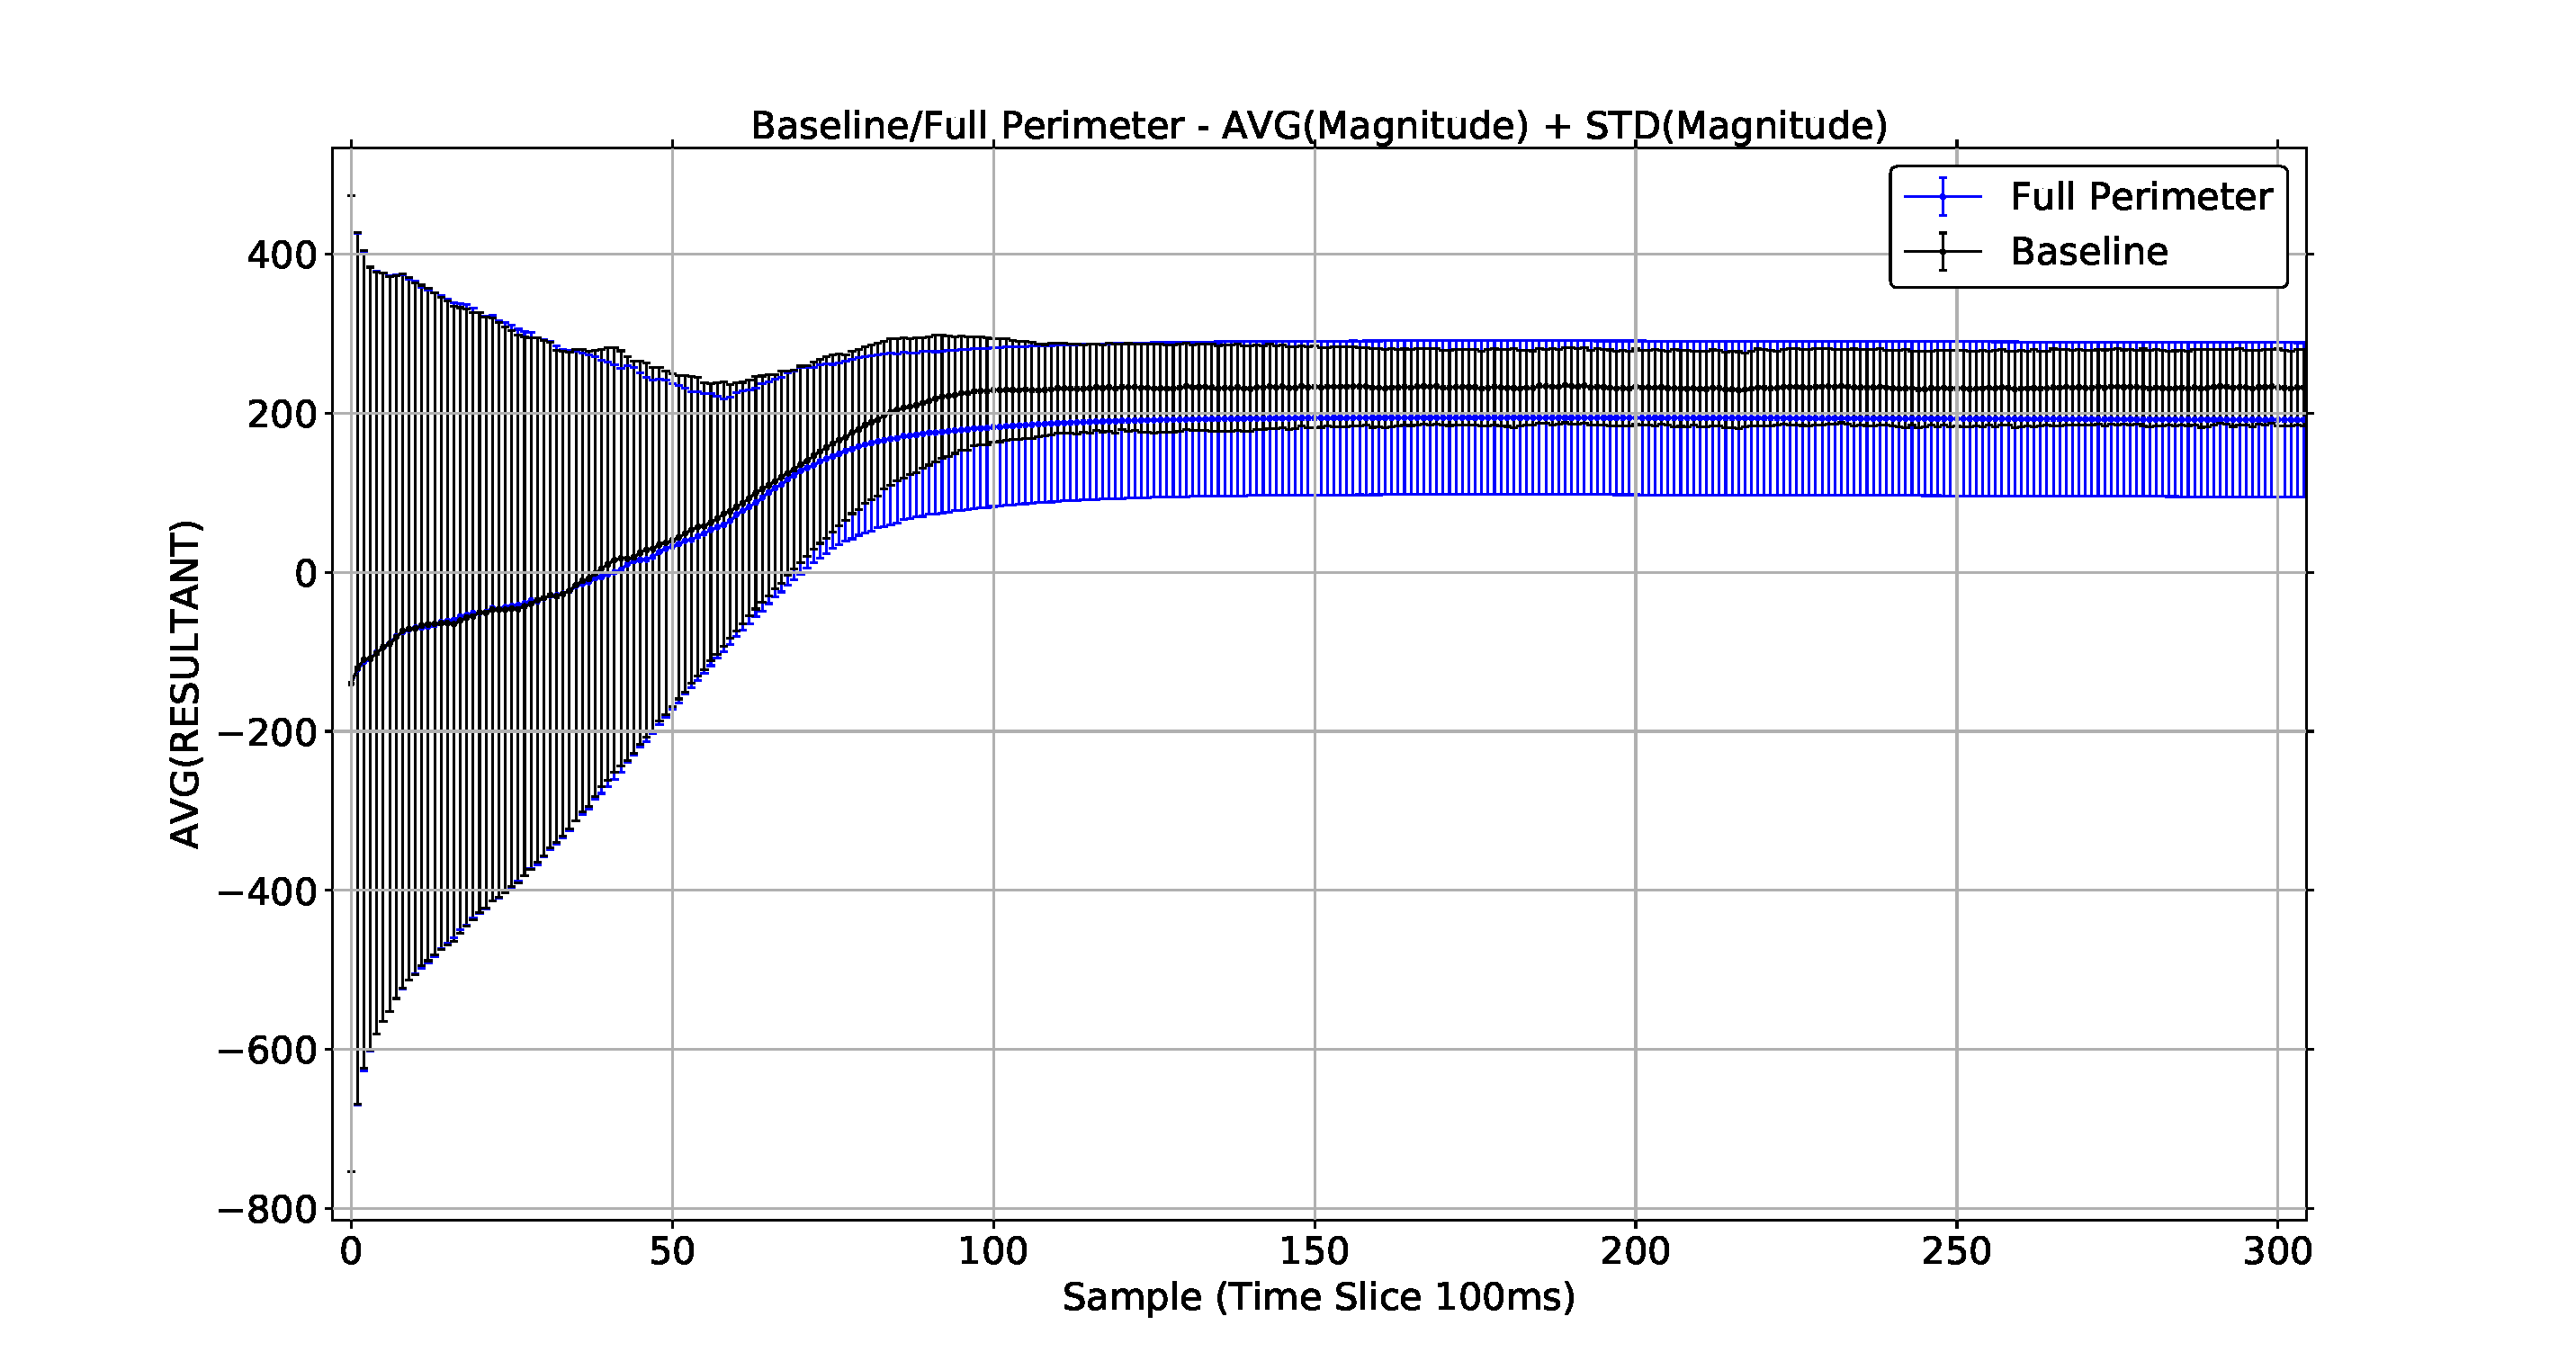
\includegraphics[width=14cm]{CHAPTER-6/figures/BaselineFullPerimeterMag1}
\end{center}
\caption{Baseline/Full perimeter magnitude comparison\label{reduced:BaselineFullPerimeterMag1}}
\end{figure}

Figure~\ref{reduced:BaselineFullPerimeterMag1} shows the magnitude metric for the simulation. Up to the point where the magnitude reaches zero ($\approx$ 4.8 seconds / 48 cycles) the swarm is undergoing expansion and the \textit{inter-agent vectors} have a higher repulsive magnitude. Up to this point it is not possible to determine if the swarm is a cohesive entity. Once the \textit{inter-agent vector magnitude} becomes positive the swarm is known to be cohesive. Once the \textit{interaction vectors' magnitudes} subside the directional bias from the coordinator agents' \textit{destination vectors} will influence the swarm's direction. 

Once the swarm has completed its expansion the swarm's interacting vectors stabilise to an optimum level for the swarm environment parameters. The level of interaction between the vectors produces an increase in the jitter compared to the baseline. This change is induced by the coordinators' \textit{destination vectors}.

\begin{figure}[H]
\begin{center}
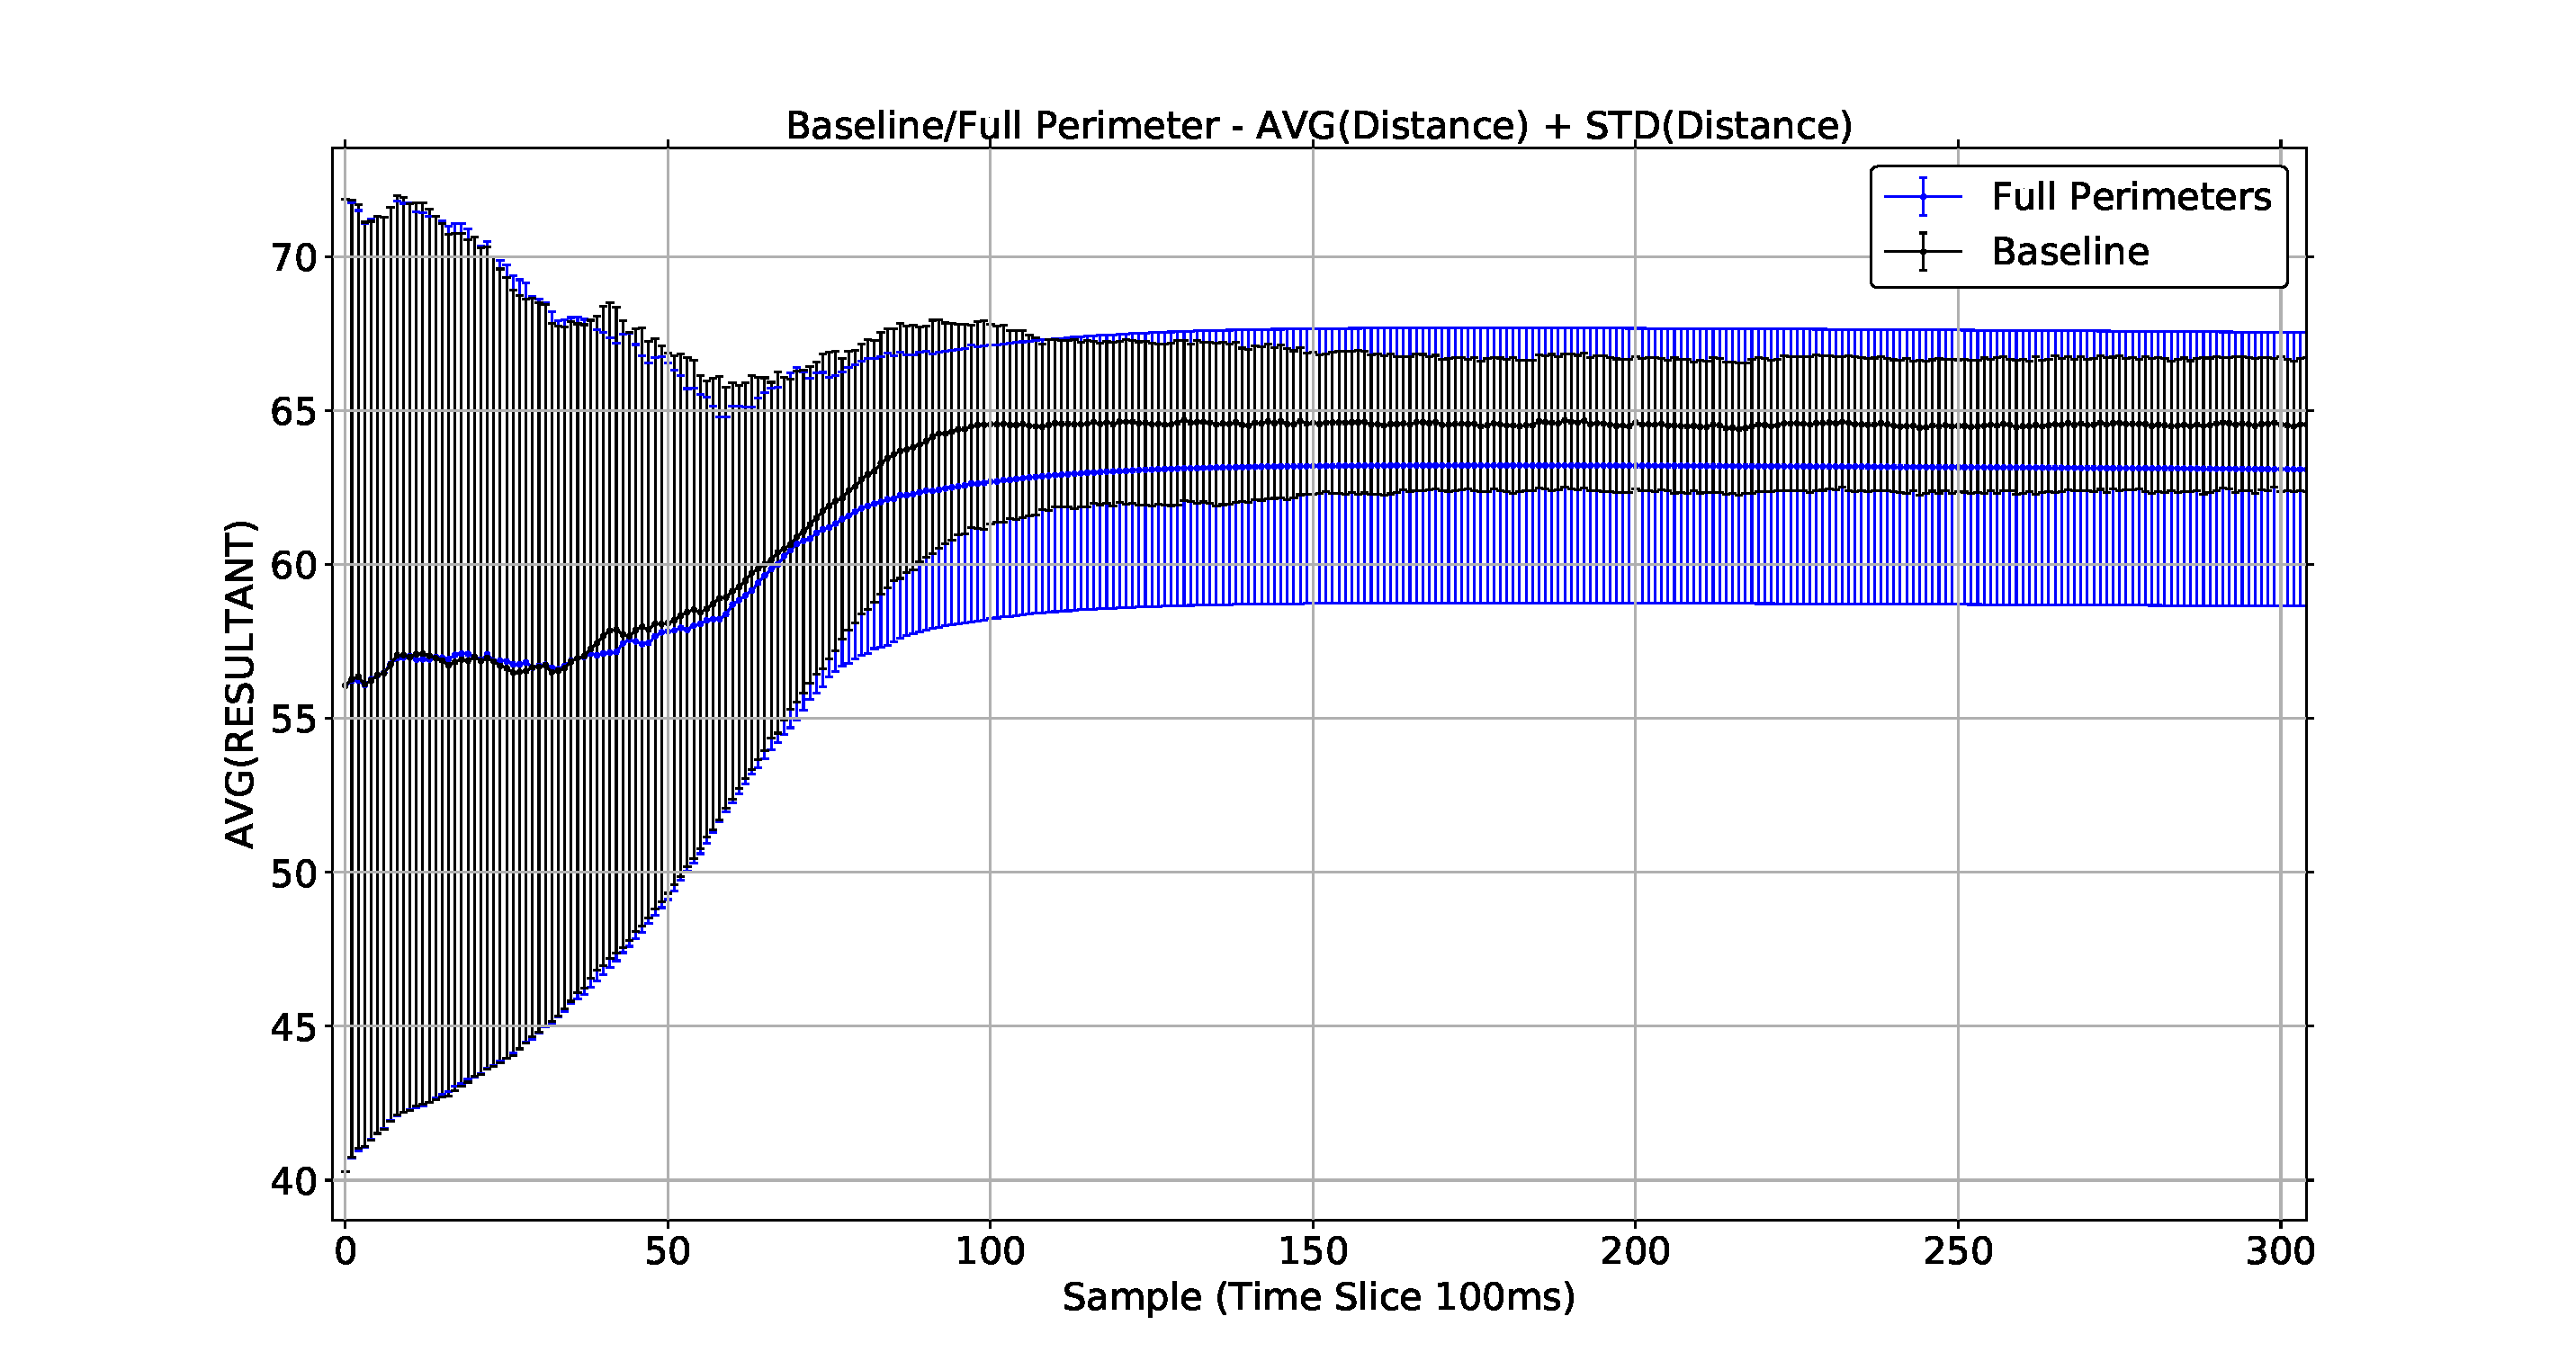
\includegraphics[width=14cm]{CHAPTER-6/figures/BaselineFullPerimeterDist1}
\end{center}
\caption{Baseline/Full perimeter distance comparison\label{reduced:BaselineFullPerimeterDist1}}
\end{figure}

Figure~\ref{reduced:BaselineFullPerimeterDist1} shows the swarm expanding as the average distance increases. The expansion eventually settles to a level where the agents are separated but the average distribution is less than the baseline. The reduction in the inter-agent distances is caused by a change induced by the \textit{destination vectors} of the coordinators reducing the repulsion effect. The level of jitter is also greater than the baseline again this is caused by the \textit{destination vectors} preventing the non-coordinator agents from moving towards an equilibrium state.

\subsection{Complex Multifaceted Swarm (full-perimeter) - Simulation}
The simulation shows that once the swarm has stabilised the majority of agents are still disrupted by the introduction of the \textit{destination vectors}. This results in the swarm's agents having to move more to maintain the hexagonal structures. The agents that are on the perimeter tend to have 3 or more neighbours. 

The experiment demonstrates that the perimeter detection algorithm is a practical technique to apply to the detection of a swarm subset to reduce GPS usage. However the environmental parameters the impact of the \textit{destination vectors}create a high level of jitter within the swarm.

\section{Baseline and effect comparison\label{section:compareBaselineAll1}}
To compare the three algorithms and their effects the metric defined in chapter~\ref{chapter:metric} is combined with the swarm's emergent properties. The internal movement (jitter), the terminal speed of the centroid of the swarm and the effect on the path of the swarm are considered. 

Analysing the path and speed of a swarm requires the centroid to be identified~\cite{HAY:08,VG:05,GP:02,GP:04,GP:04a,GP:05,GP:11}. The centroid is then tracked over time as the swarm progresses towards it's goal~(Equation~\ref{eq:Centroid1}).

The centroid of the swarm is determined by taking the coordinate position of each agent and calculating the mean of the $x$ and $y$ positions.

\begin{equation}\label{eq:Centroid1}
C_s = \frac{1}{\card{S}}\mathlarger{\sum_{b' \in S}} b'
\end{equation}‎

Equation~\ref{eq:Centroid1} calculates the coordinates for the centre of the swarm ($C_s$) as an $x,y$ coordinate where $S$ is the swarm and $b^{'}$ is the coordinate $x,y$ for each agent and $\card{S}$ is the number of agents in the swarm.

Comparing swarms with these metrics generates a fuller understanding of the effects the algorithms and allows suitable applications to be identified.

\subsection{Internal movement comparison\label{section:stabilityComparison1}}
Figures \ref{reduced:BaselineAllDist1}, \ref{reduced:BaselineAllDist2}, \ref{reduced:BaselineAllMag1}, and \ref{reduced:BaselineAllMag2} identify the jitter based on distance and the \textit{inter-agent vector magnitudes} for the coordination algorithms and the baseline. Both the metrics show that as the number of coordinator agents increases the jitter increases. 

\begin{figure}[H]
\begin{center}
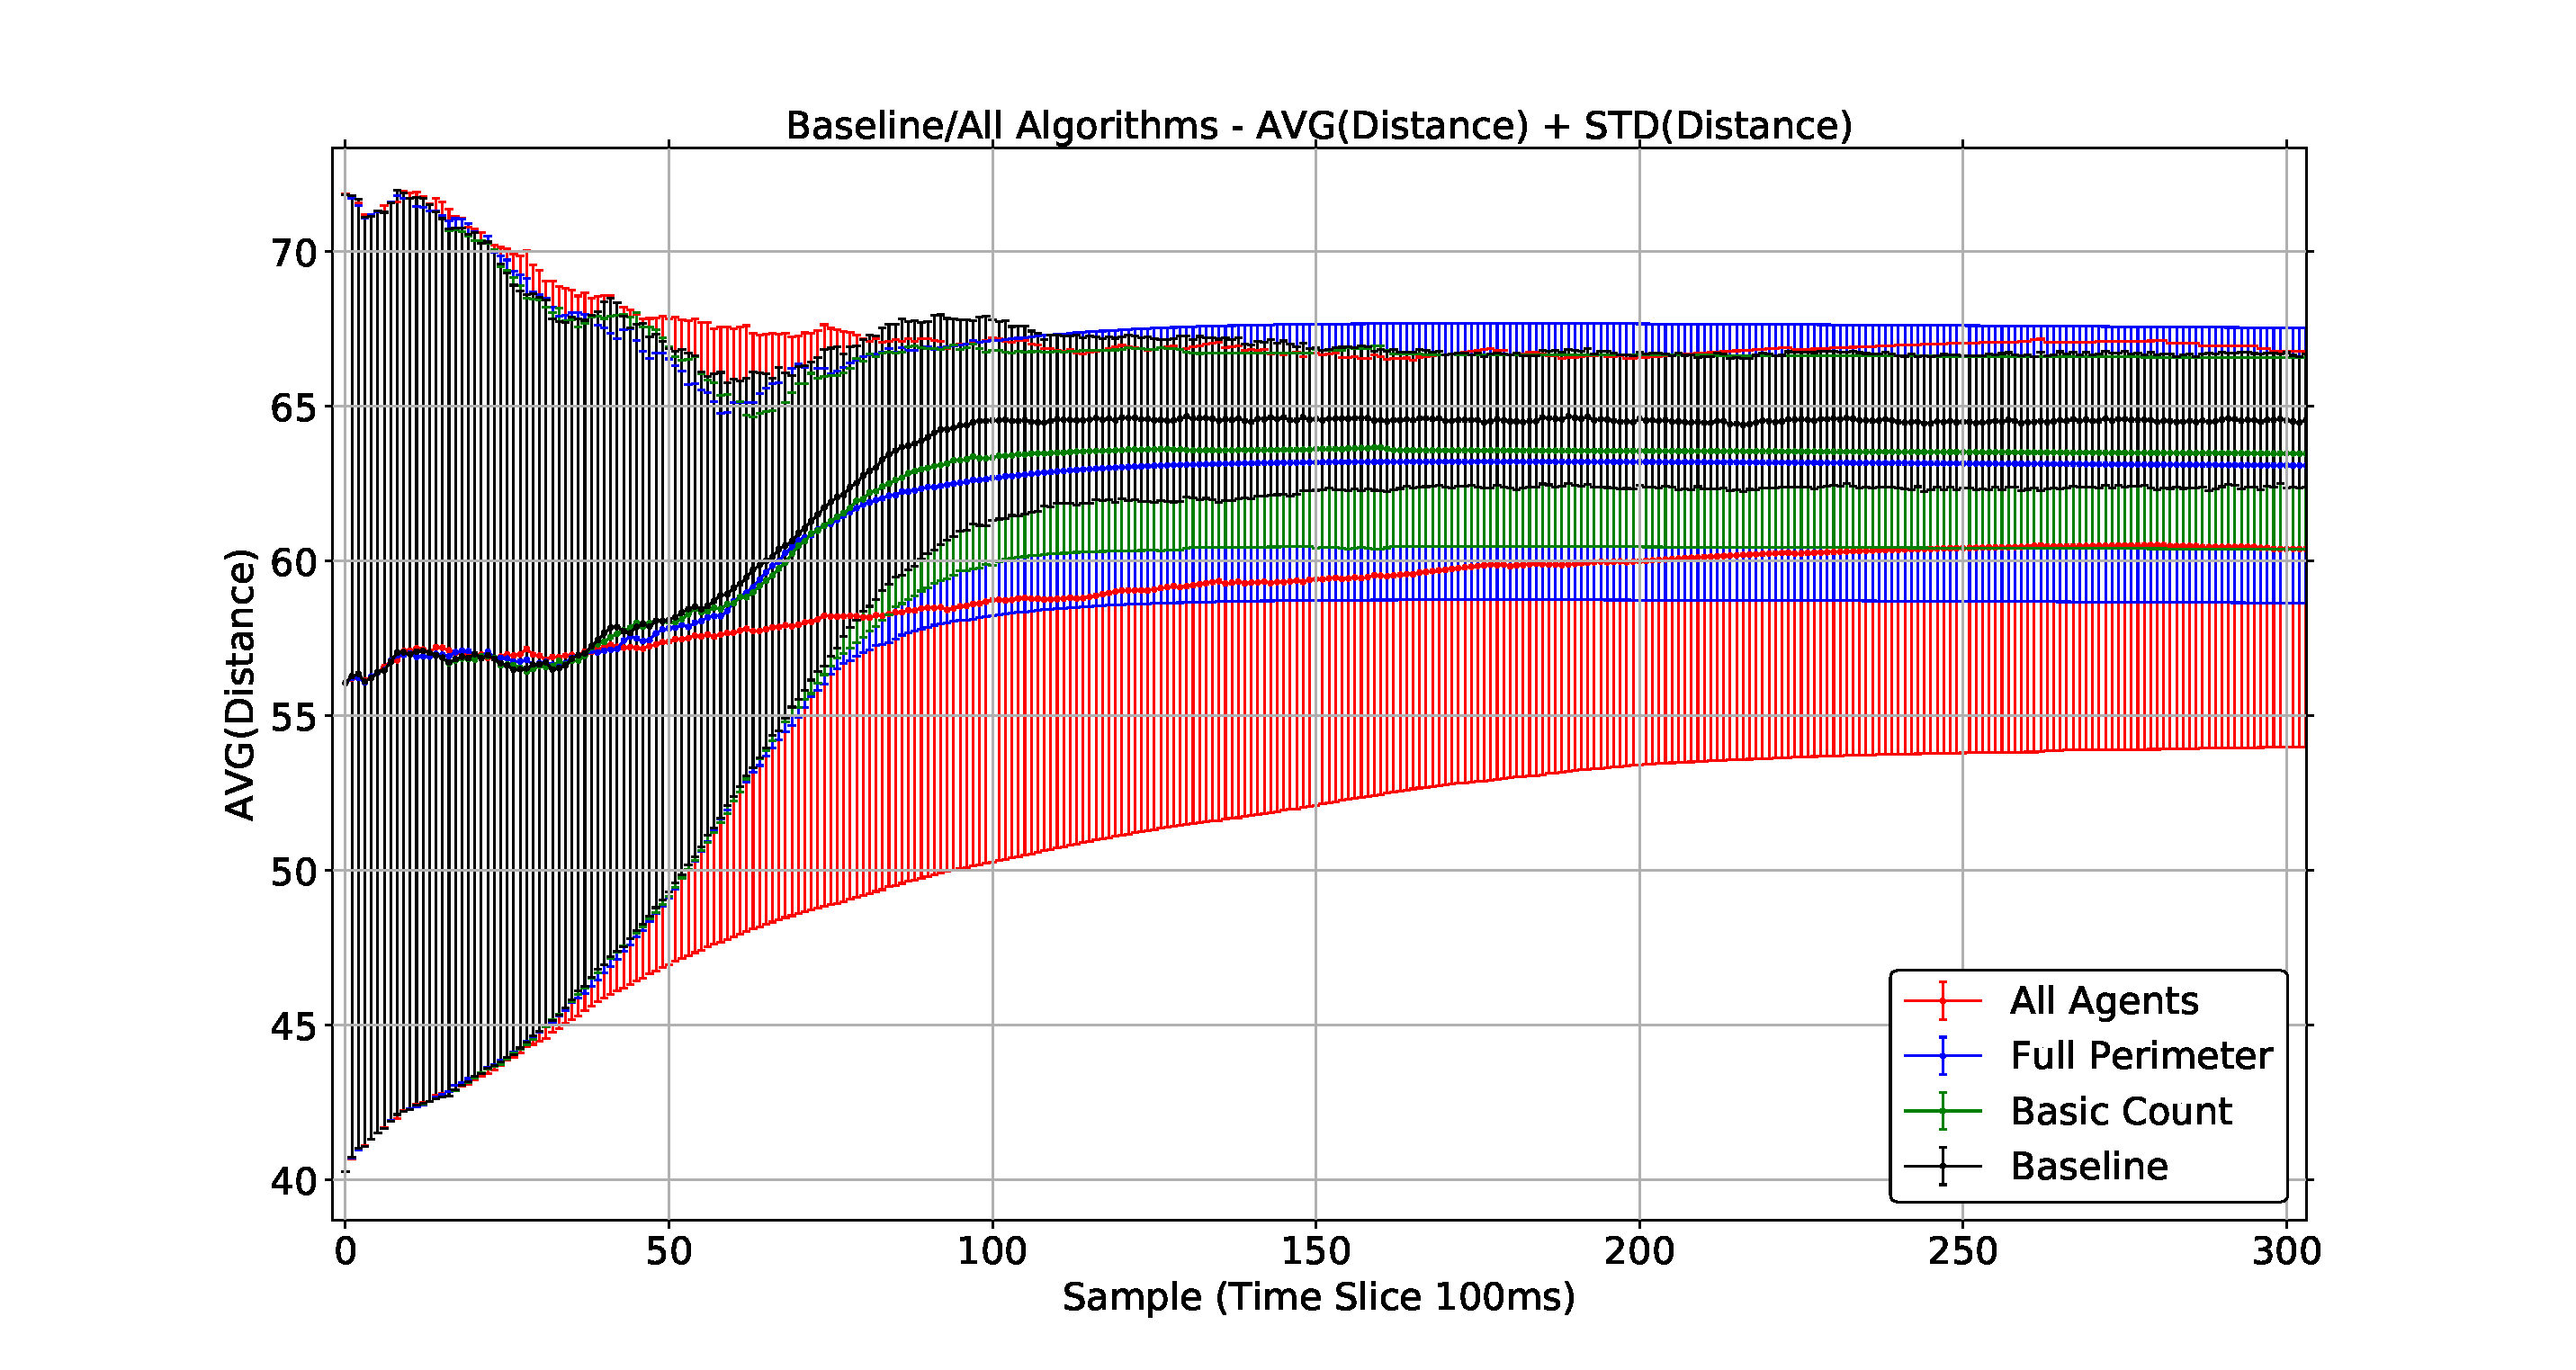
\includegraphics[width=14cm]{CHAPTER-6/figures/BaselineAllDist1}
\end{center}
\caption{Baseline distance comparison\label{reduced:BaselineAllDist1}}
\end{figure}

\begin{figure}[H]
\begin{center}
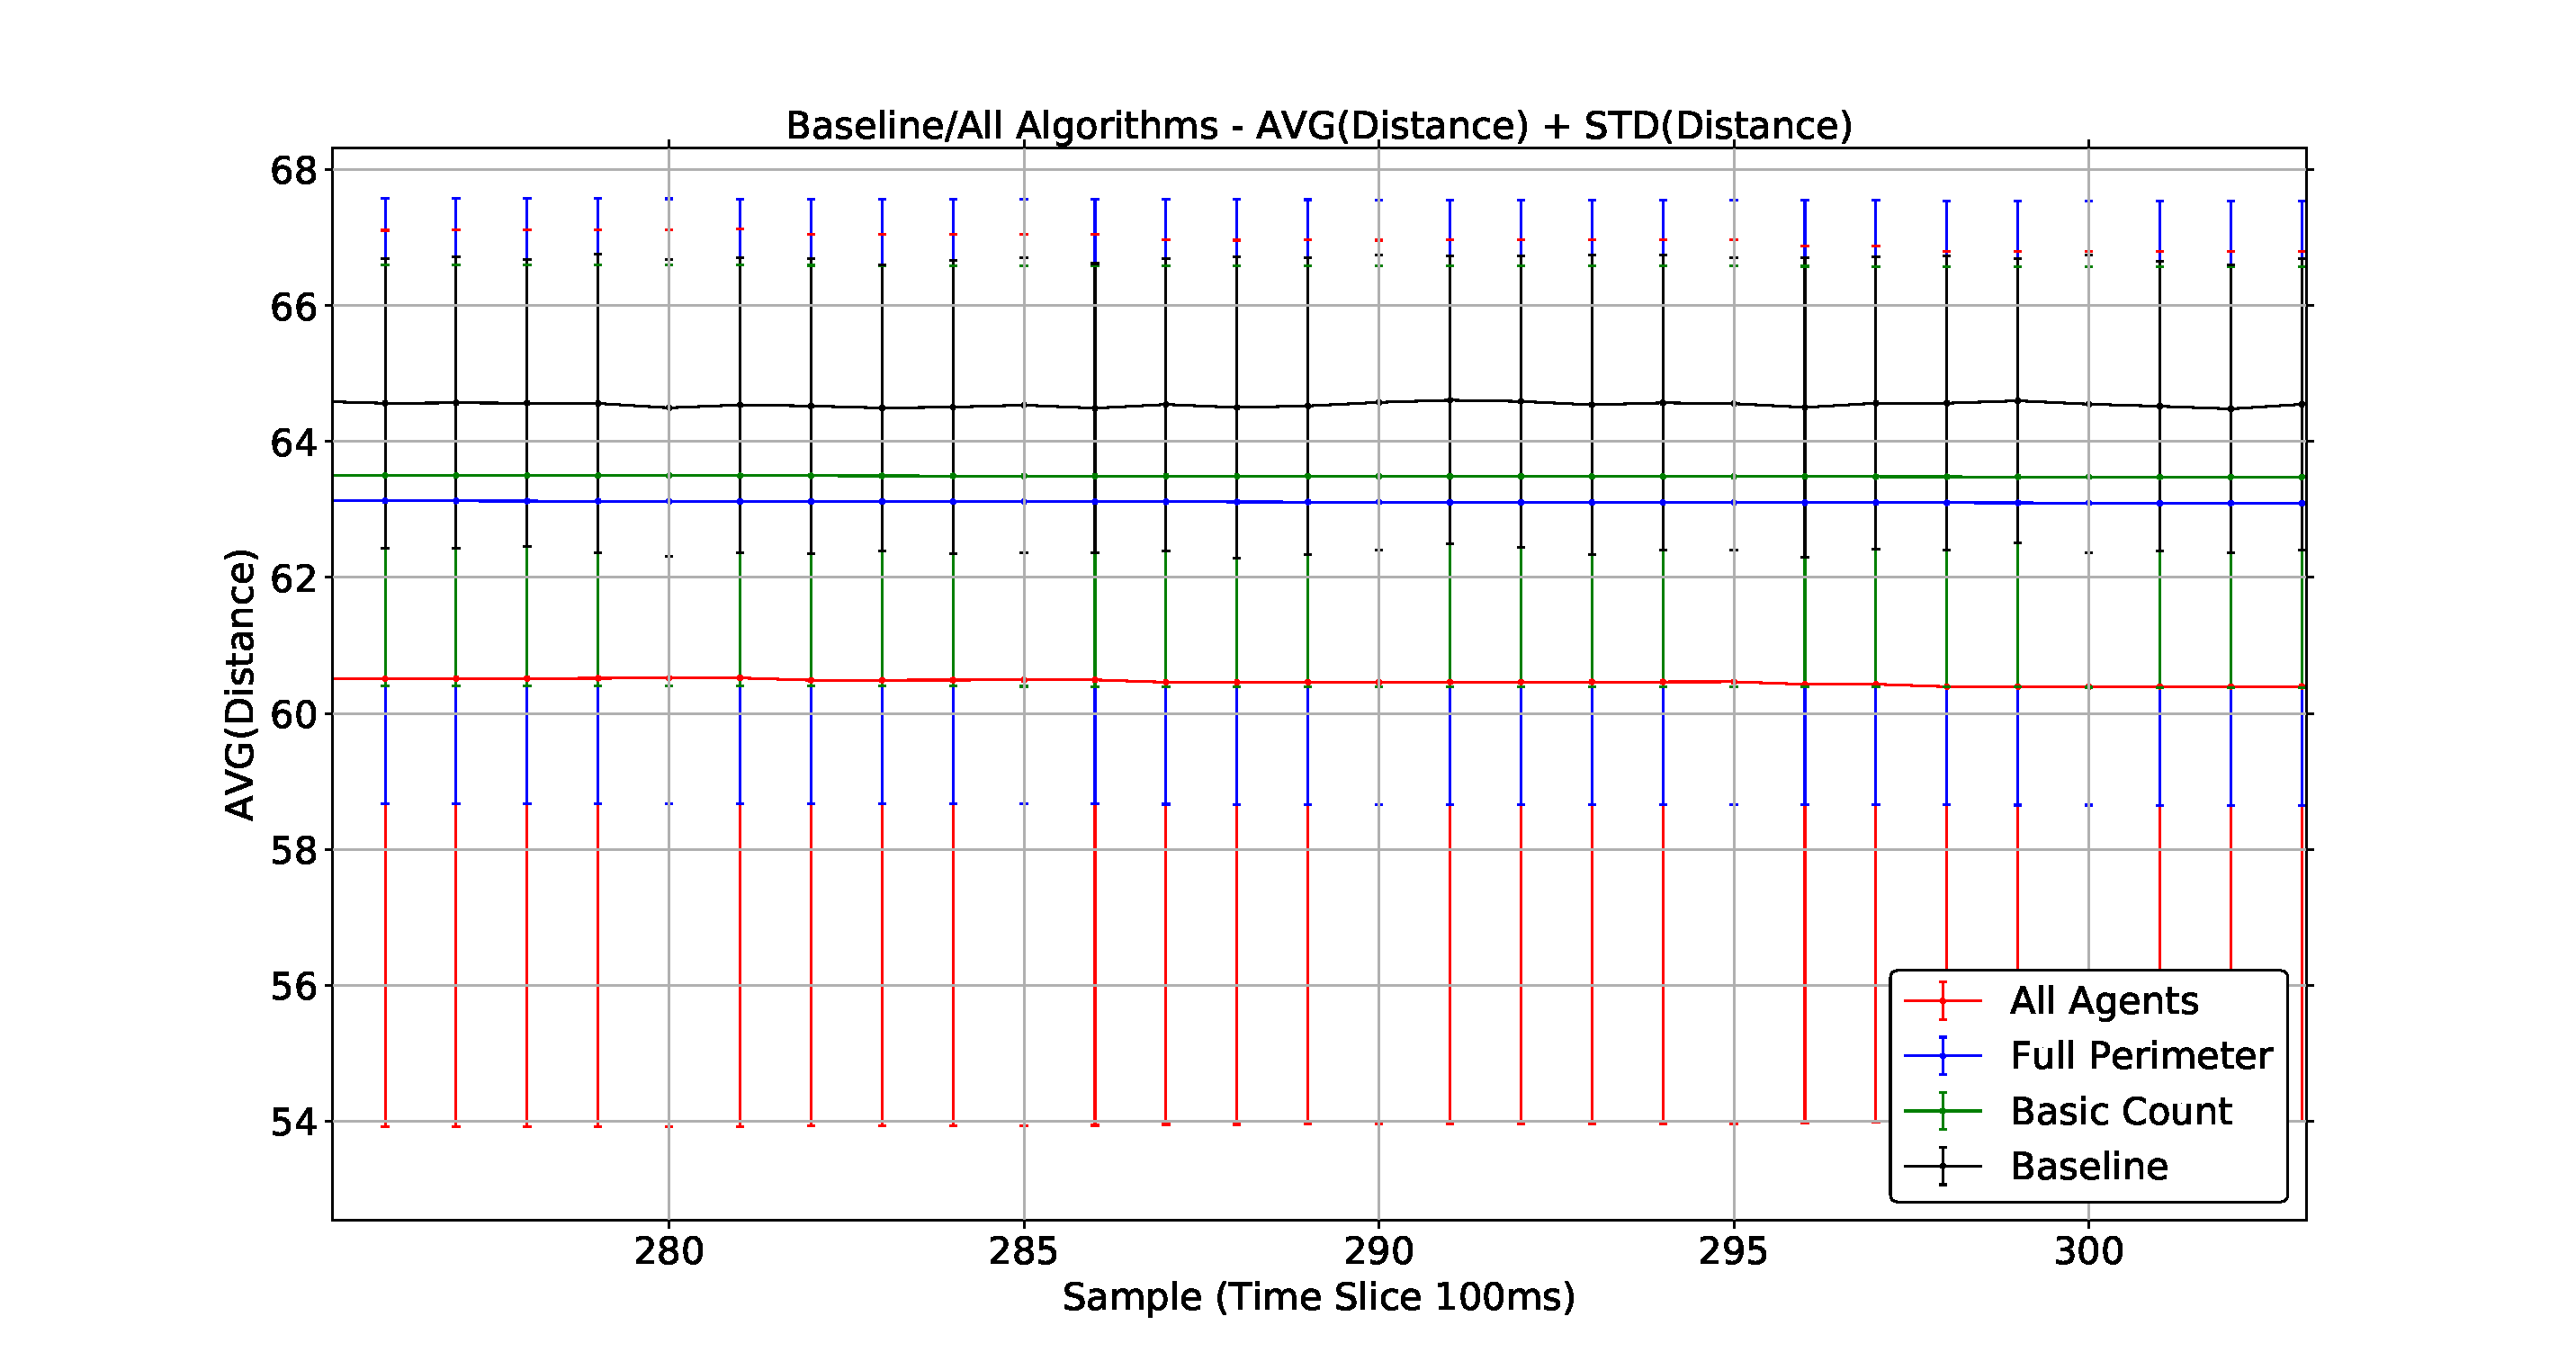
\includegraphics[width=14cm]{CHAPTER-6/figures/BaselineAllDist2}
\end{center}
\caption{Baseline distance comparison\label{reduced:BaselineAllDist2}}
\end{figure}

Figure~\ref{reduced:BaselineAllDist2} show that the average distance between the agents is reduced when less coordinators are used. This indicates that for the same sized swarm with the same field effects the area covered by the swarm is reduced as the effect of the repulsion is hampered by the coordinators. It also shows that the time taken for the swarm to stabilises is increased due to the \textit{destination vectors} impacting on the agents ability to produce stable structures~(Figure~\ref{reduced:BaselineAllDist1}). 

\begin{figure}[H]
\begin{center}
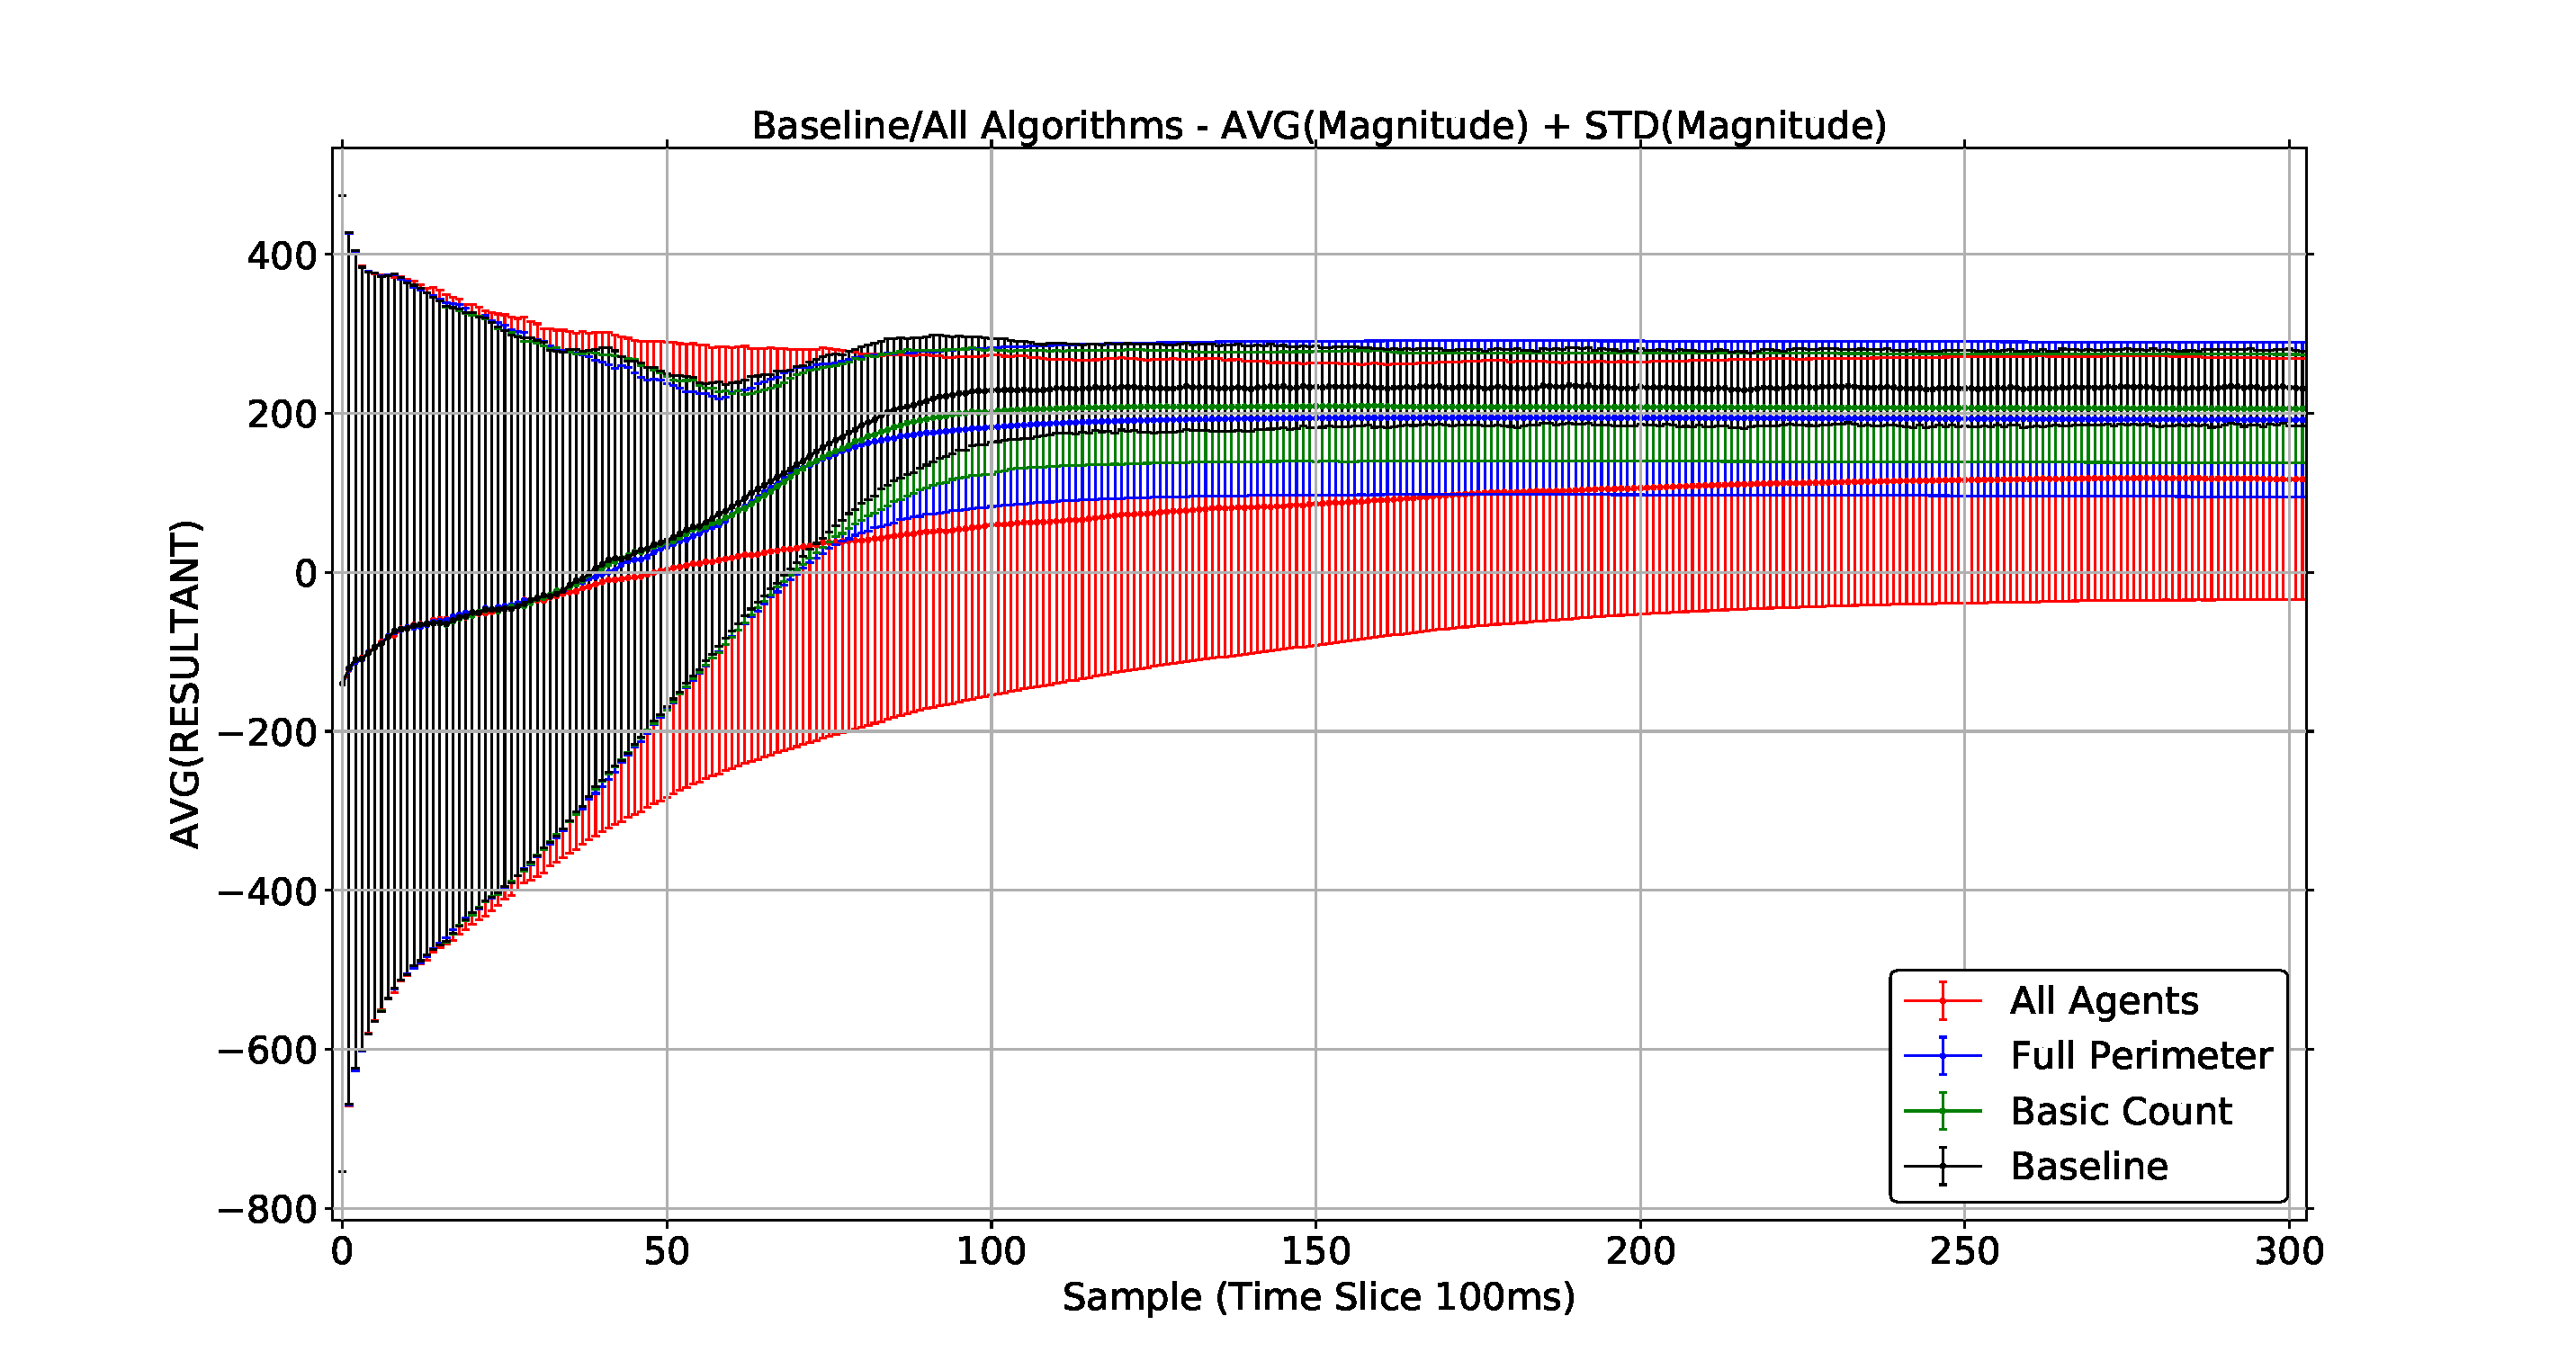
\includegraphics[width=14cm]{CHAPTER-6/figures/BaselineAllMag1}
\end{center}
\caption{Baseline magnitude comparison\label{reduced:BaselineAllMag1}}
\end{figure}

\begin{figure}[H]
\begin{center}
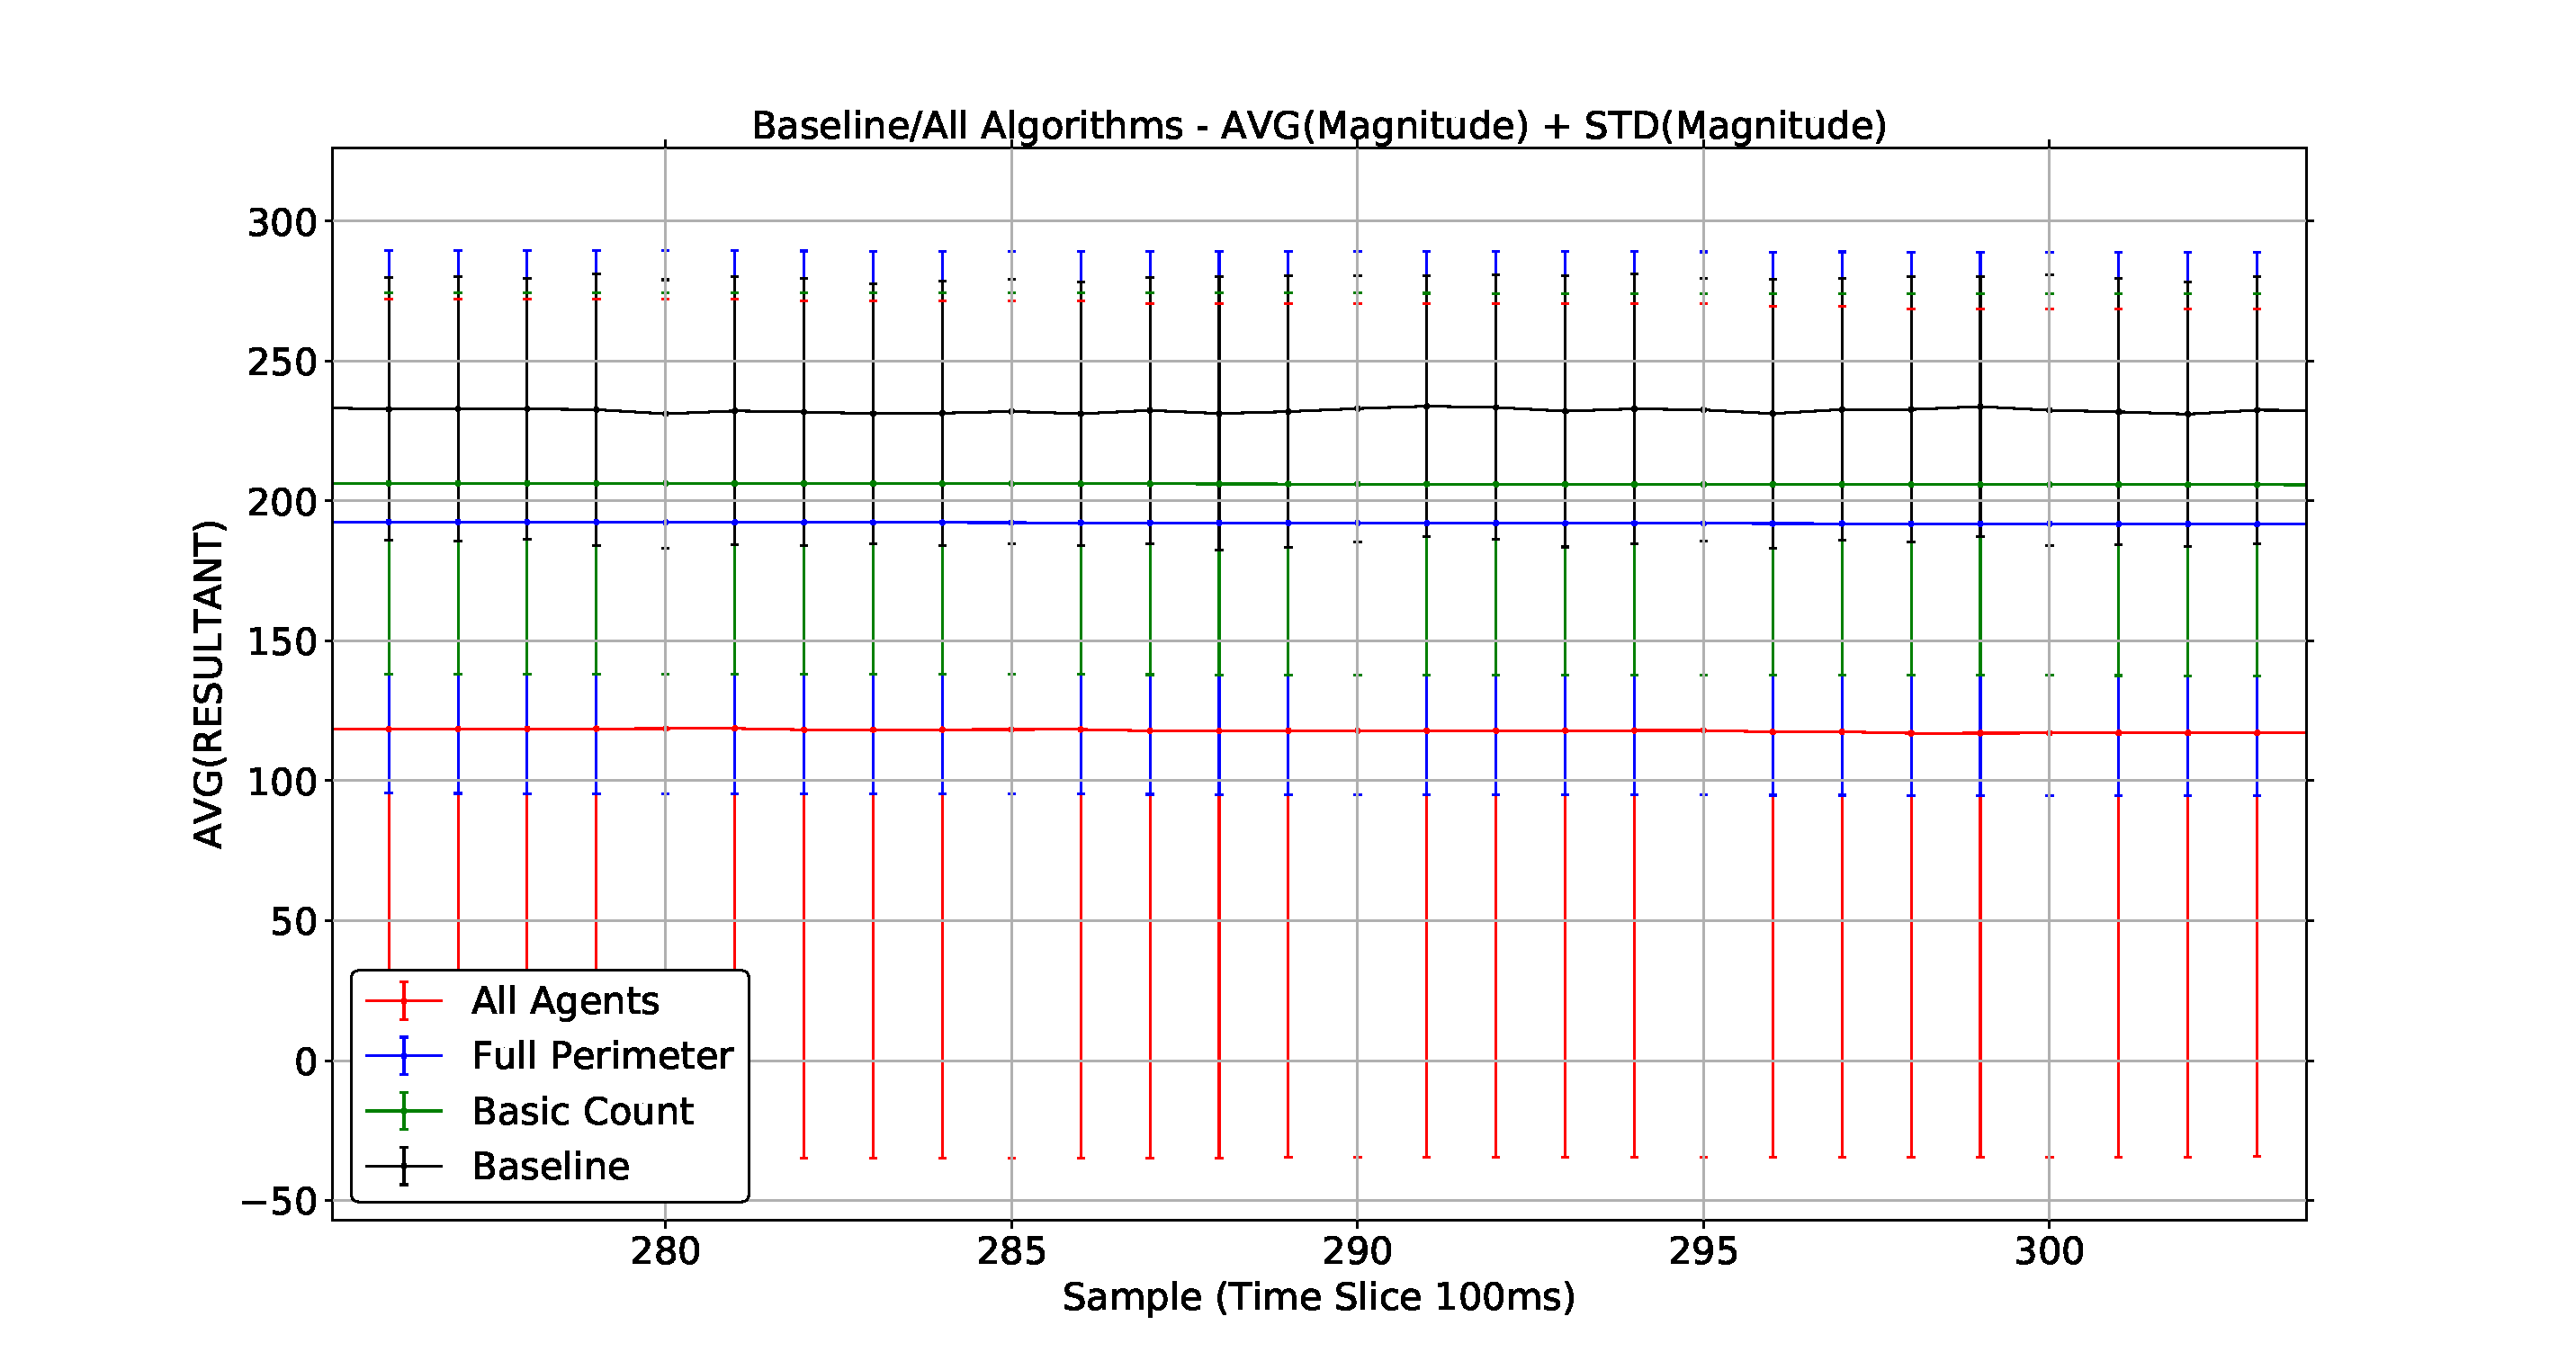
\includegraphics[width=14cm]{CHAPTER-6/figures/BaselineAllMag2}
\end{center}
\caption{Baseline and magnitude comparison\label{reduced:BaselineAllMag2}}
\end{figure}

Figures \ref{reduced:BaselineAllMag1} and \ref{reduced:BaselineAllMag2} highlight that a highly compressed swarm's magnitude, indicated by a negative magnitude, will overwhelm most of a swarm's activity. This can be expected due to the size of the magnitudes that are affecting the swarm's movement. When all agents in a swarm are coordinators the directional effect can break through the highly cohesive stabilising vectors but this increases the level of jitter making the swarm's internal movement less predictable.

The directional algorithm that introduces the least amount of jitter is the basic-count algorithm. The basic-count algorithm is also the simplest of the multi-faceted algorithms to implement with a minimal computational overhead for the agents. 

Figure~\ref{reduced:BaselineAllMag2} shows a closer view of the swarms following the stabilisation period between 17.5s and 20s. The basic-count algorithm produces the least disruption to the agents and has the highest average \textit{inter-agent vector magnitude} indicating the swarm has a higher tendency to remain cohesive with the widest distribution. This effect is caused by the increase in the cohesion effect when the agents are more distant. This demonstrates that the algorithm produces a swarm that covers a greater area. The increased area coverage is confirmed by figure~\ref{reduced:BaselineAllDist2} which shown the greatest average inter-agent distance. The `all-agent' algorithm has the smallest resultant \textit{inter-agent vector magnitude} indicating that the swarm is more highly compressed (more repulsion is in operation). This is corroborated by the inter-agent distribution shown in~figure~\ref{reduced:BaselineAllDist2}.

\subsection{Swarm GPS utilisation\label{section:compareGPSUages1}}
The multi-faceted algorithms that are defined above create subsets of coordinator agents for the application of a \textit{destination vector} bias of a swarm. These subsets can be identified to identify the GPS usage in the swarm at each time cycle ($t$). This allows a profile of the algorithms' coordinator role identification process to be isolated to identify the level of GPS utilisation in the swarm.

\begin{figure}[H]
\begin{center}
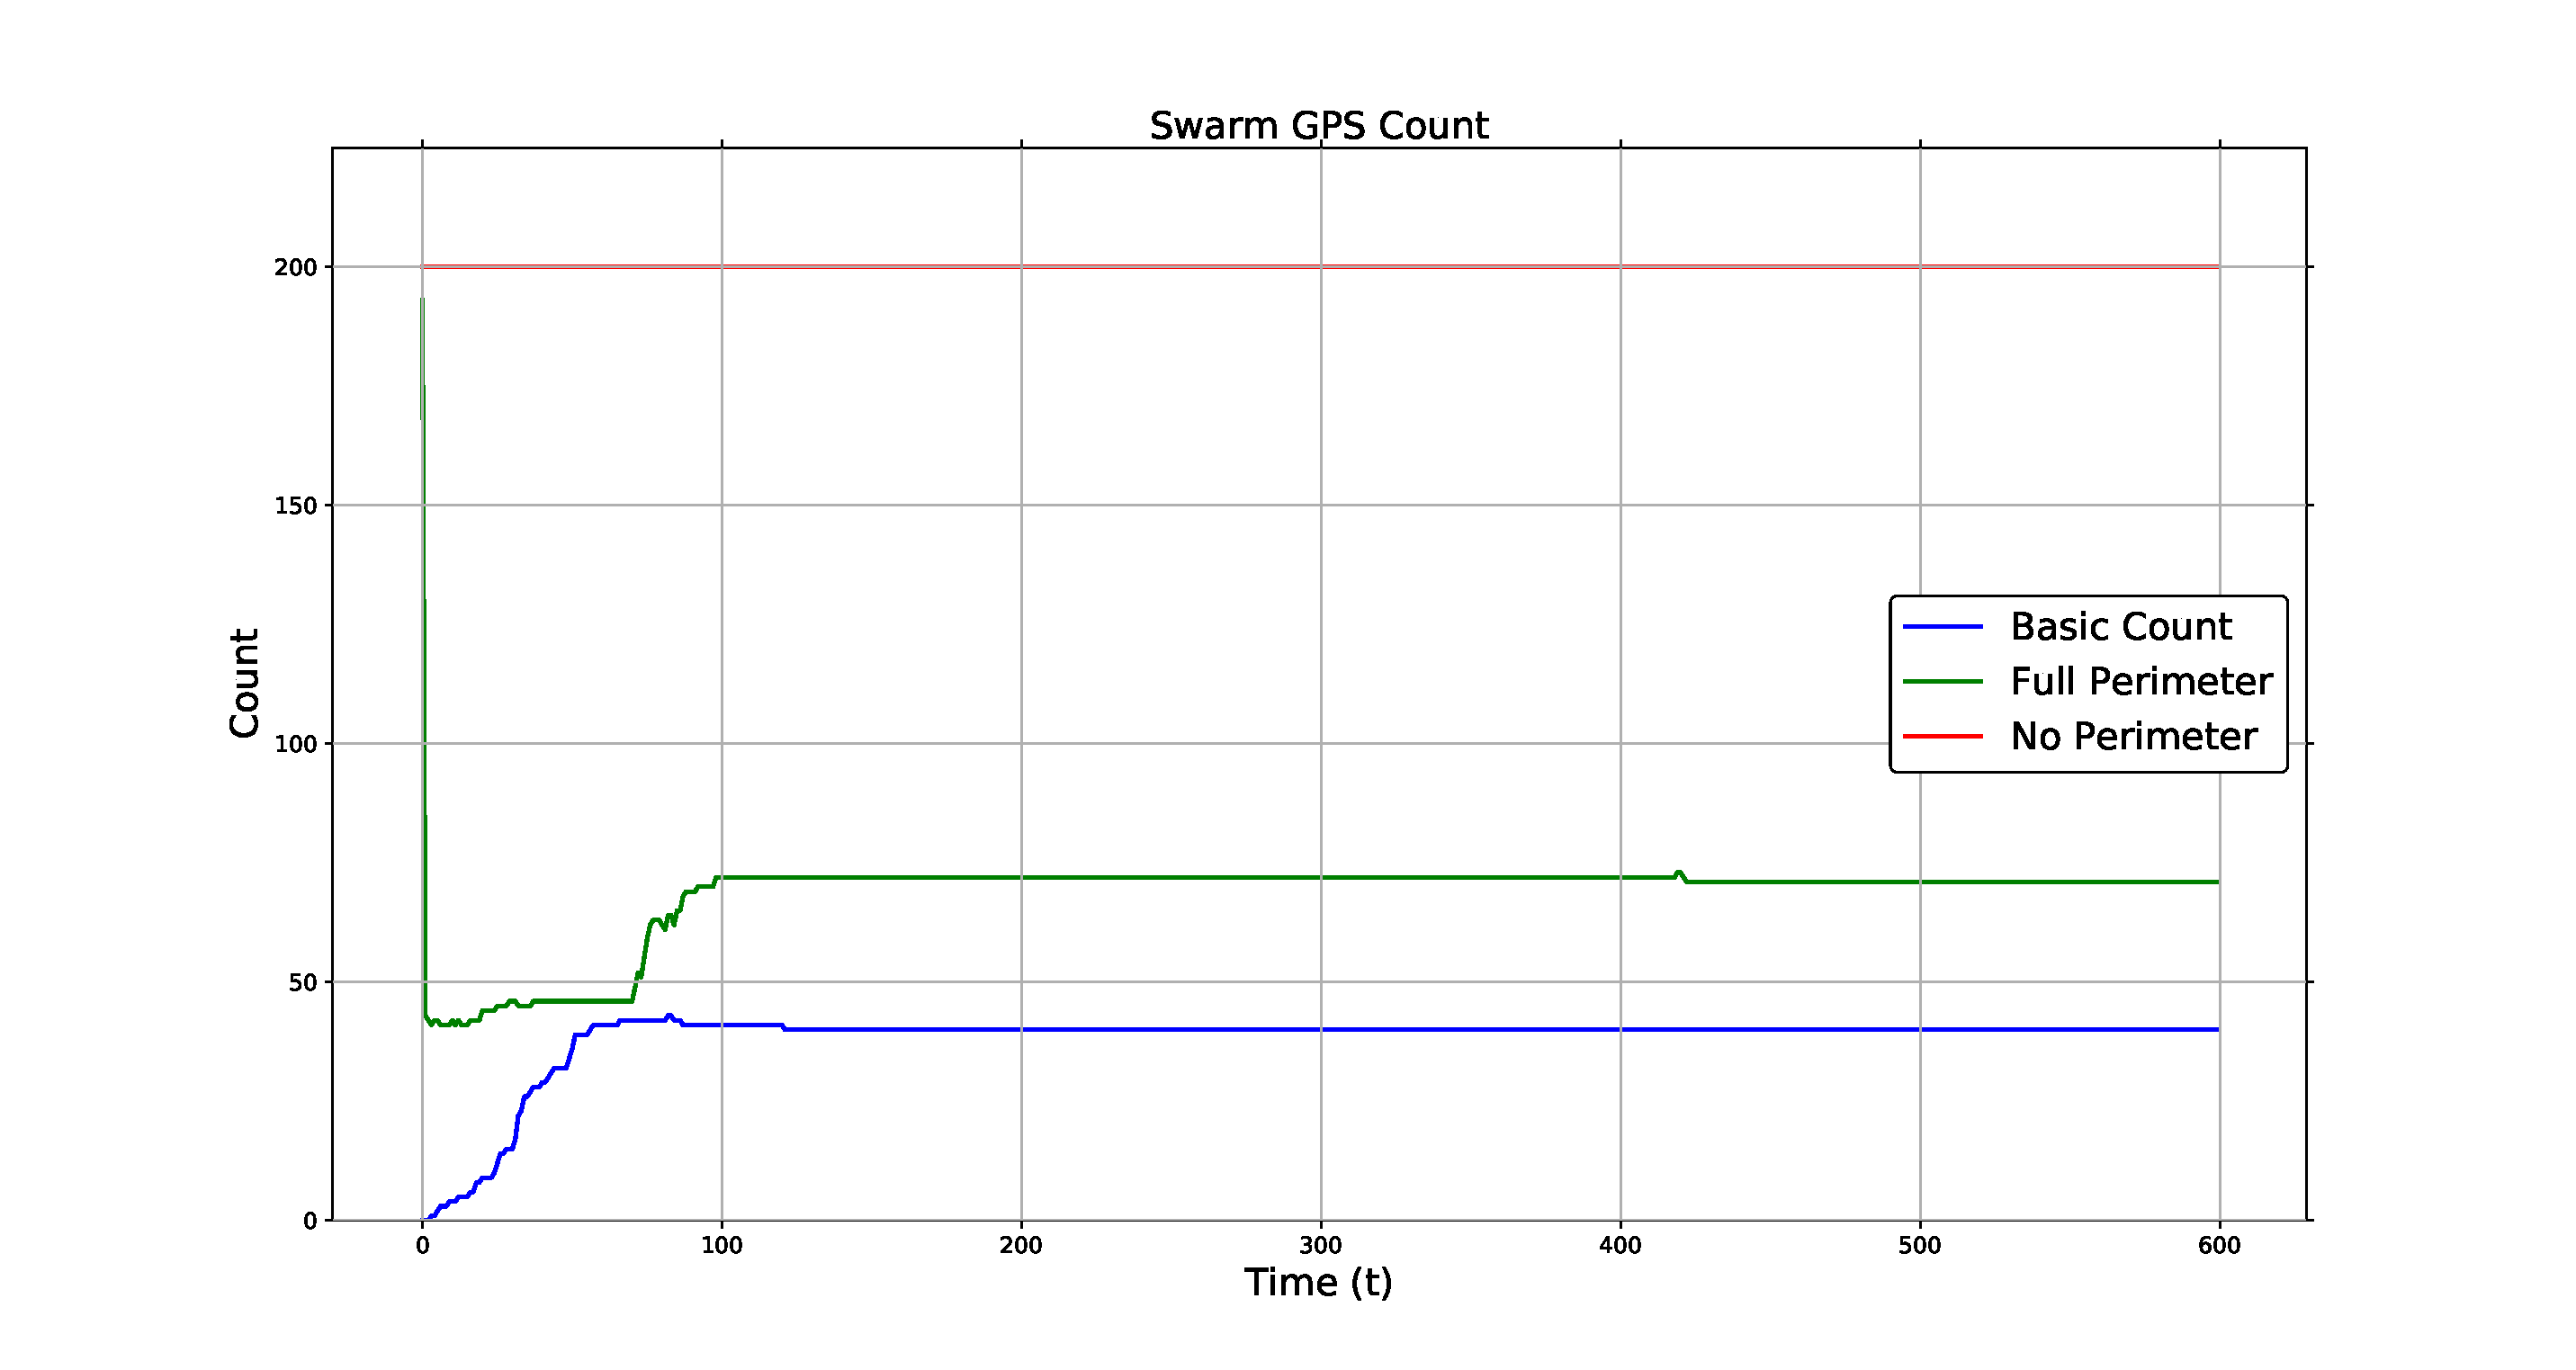
\includegraphics[width=14cm]{CHAPTER-6/figures/SwarmPerimeter1}
\end{center}
\caption{200 agent swarm GPS Usage\label{fig:SwarmPerimeter1}}
\end{figure}

Figure~\ref{fig:SwarmPerimeter1} shows the development of the GPS utilisation of the swarm using the `all-agent' coordination and the perimeter detection (multi-faceted) algorithms over the period of a 60s simulation. 

\subsubsection{All agent GPS utilisation\label{section:SwarmPerimeter2}}
Figure~\ref{fig:SwarmPerimeter1} shows the `all-agent' algorithm as a simple flat constant of 200 agents which is 100\% of the swarm's agents. The directional bias is therefore constant throughout the simulation. 

\subsubsection{Basic-count GPS utilisation\label{section:SwarmPerimeter3}}
In~figure~\ref{fig:SwarmPerimeter1} the `basic-count' algorithm is shown in blue. Due to the swarm being compressed the basic-count effect is initially limited. There are no coordinators identified at $t=0$. This is due to the compression of the agents in the initial deployment. As the simulation progresses the disorganised stage expands the swarm and disperses the agents such that each agent develops less neighbours. The coordinator detection algorithm then begins to identify a subset on the perimeter. This process continues and eventually settles, shown by the plateau in the graph. Figure~\ref{fig:SwarmPerimeter1} shows there is a slight change in the swarm structure at 8 seconds, this is due to anomalies in the swarm being corrected by the effect of the cohesion and repulsion field effects. Once the anomalies percolate out of the swarm the structure stabilises and the number of coordinators stops fluctuating.

\subsubsection{Full perimeter GPS utilisation\label{section:SwarmPerimeter4}}
The full perimeter detection algorithm starts with a subset immediately as shown in green in figure~\ref{fig:SwarmPerimeter1}. This is due to the algorithm always detecting a full perimeter based on neighbour visibility. This has an immediate effect on the swarm as there is always a degree of \textit{destination vector magnitude} influence on the swarm, even during the expansion phase. However, the \textit{interaction vector magnitudes} are much larger than the \textit{destination vector magnitude} so the progression towards the goal is hampered and the path of the swarm is erratic. The introduction of the \textit{destination vector} influence from the very begin also disrupts the swarm's expansion and increases the duration of the disorganised period. As the swarm expands the algorithm detects more agents as coordinators as the number of perimeter agents increases.

\subsection{Swarm path propagation comparison\label{section:compareBaselineAll2}}
All algorithms do eventually settle to a stable structure (for their environment parameters) with agents distributed in lattice structures. The time taken for each algorithm to achieve their stable distribution varies. This is due to the level of influence the directional bias has on the swarm. Table~\ref{tab:GPSUsage} shows the settled coordinator distributions at 12s into the simulation.

\begin{table}[H]
\begin{center}
\begin{tabular}{| p{2.5cm} | c | c | p{5cm} |}
\hline
GPS Model & Bots GPS & \% usage & Description \\ \hline
All-agents & 200 & 100\% & All agents are coordinators \\ \hline
Basic-count & 40 & 20\% & Minimal counting algorithm\\ \hline
Full perimeter & 72 & 36\% & Void detection and perimeter (capable of supporting void reduction)\\  \hline
\end{tabular}\caption{Swarm GPS enabled coordinators} \label{tab:GPSUsage}
\end{center}
\end{table}

The three algorithms take different amounts of time to stabilise~(Figure~\ref{fig:SwarmPerimeter1}) this has an impact on how long it takes each of the algorithms to impact the swarm's movement towards the destination. This effect can be seen in~figure~\ref{reduced:SwarmPropagationPathComparison1} that shows the paths that each algorithm produces. 

\begin{figure}[H]
\begin{center}
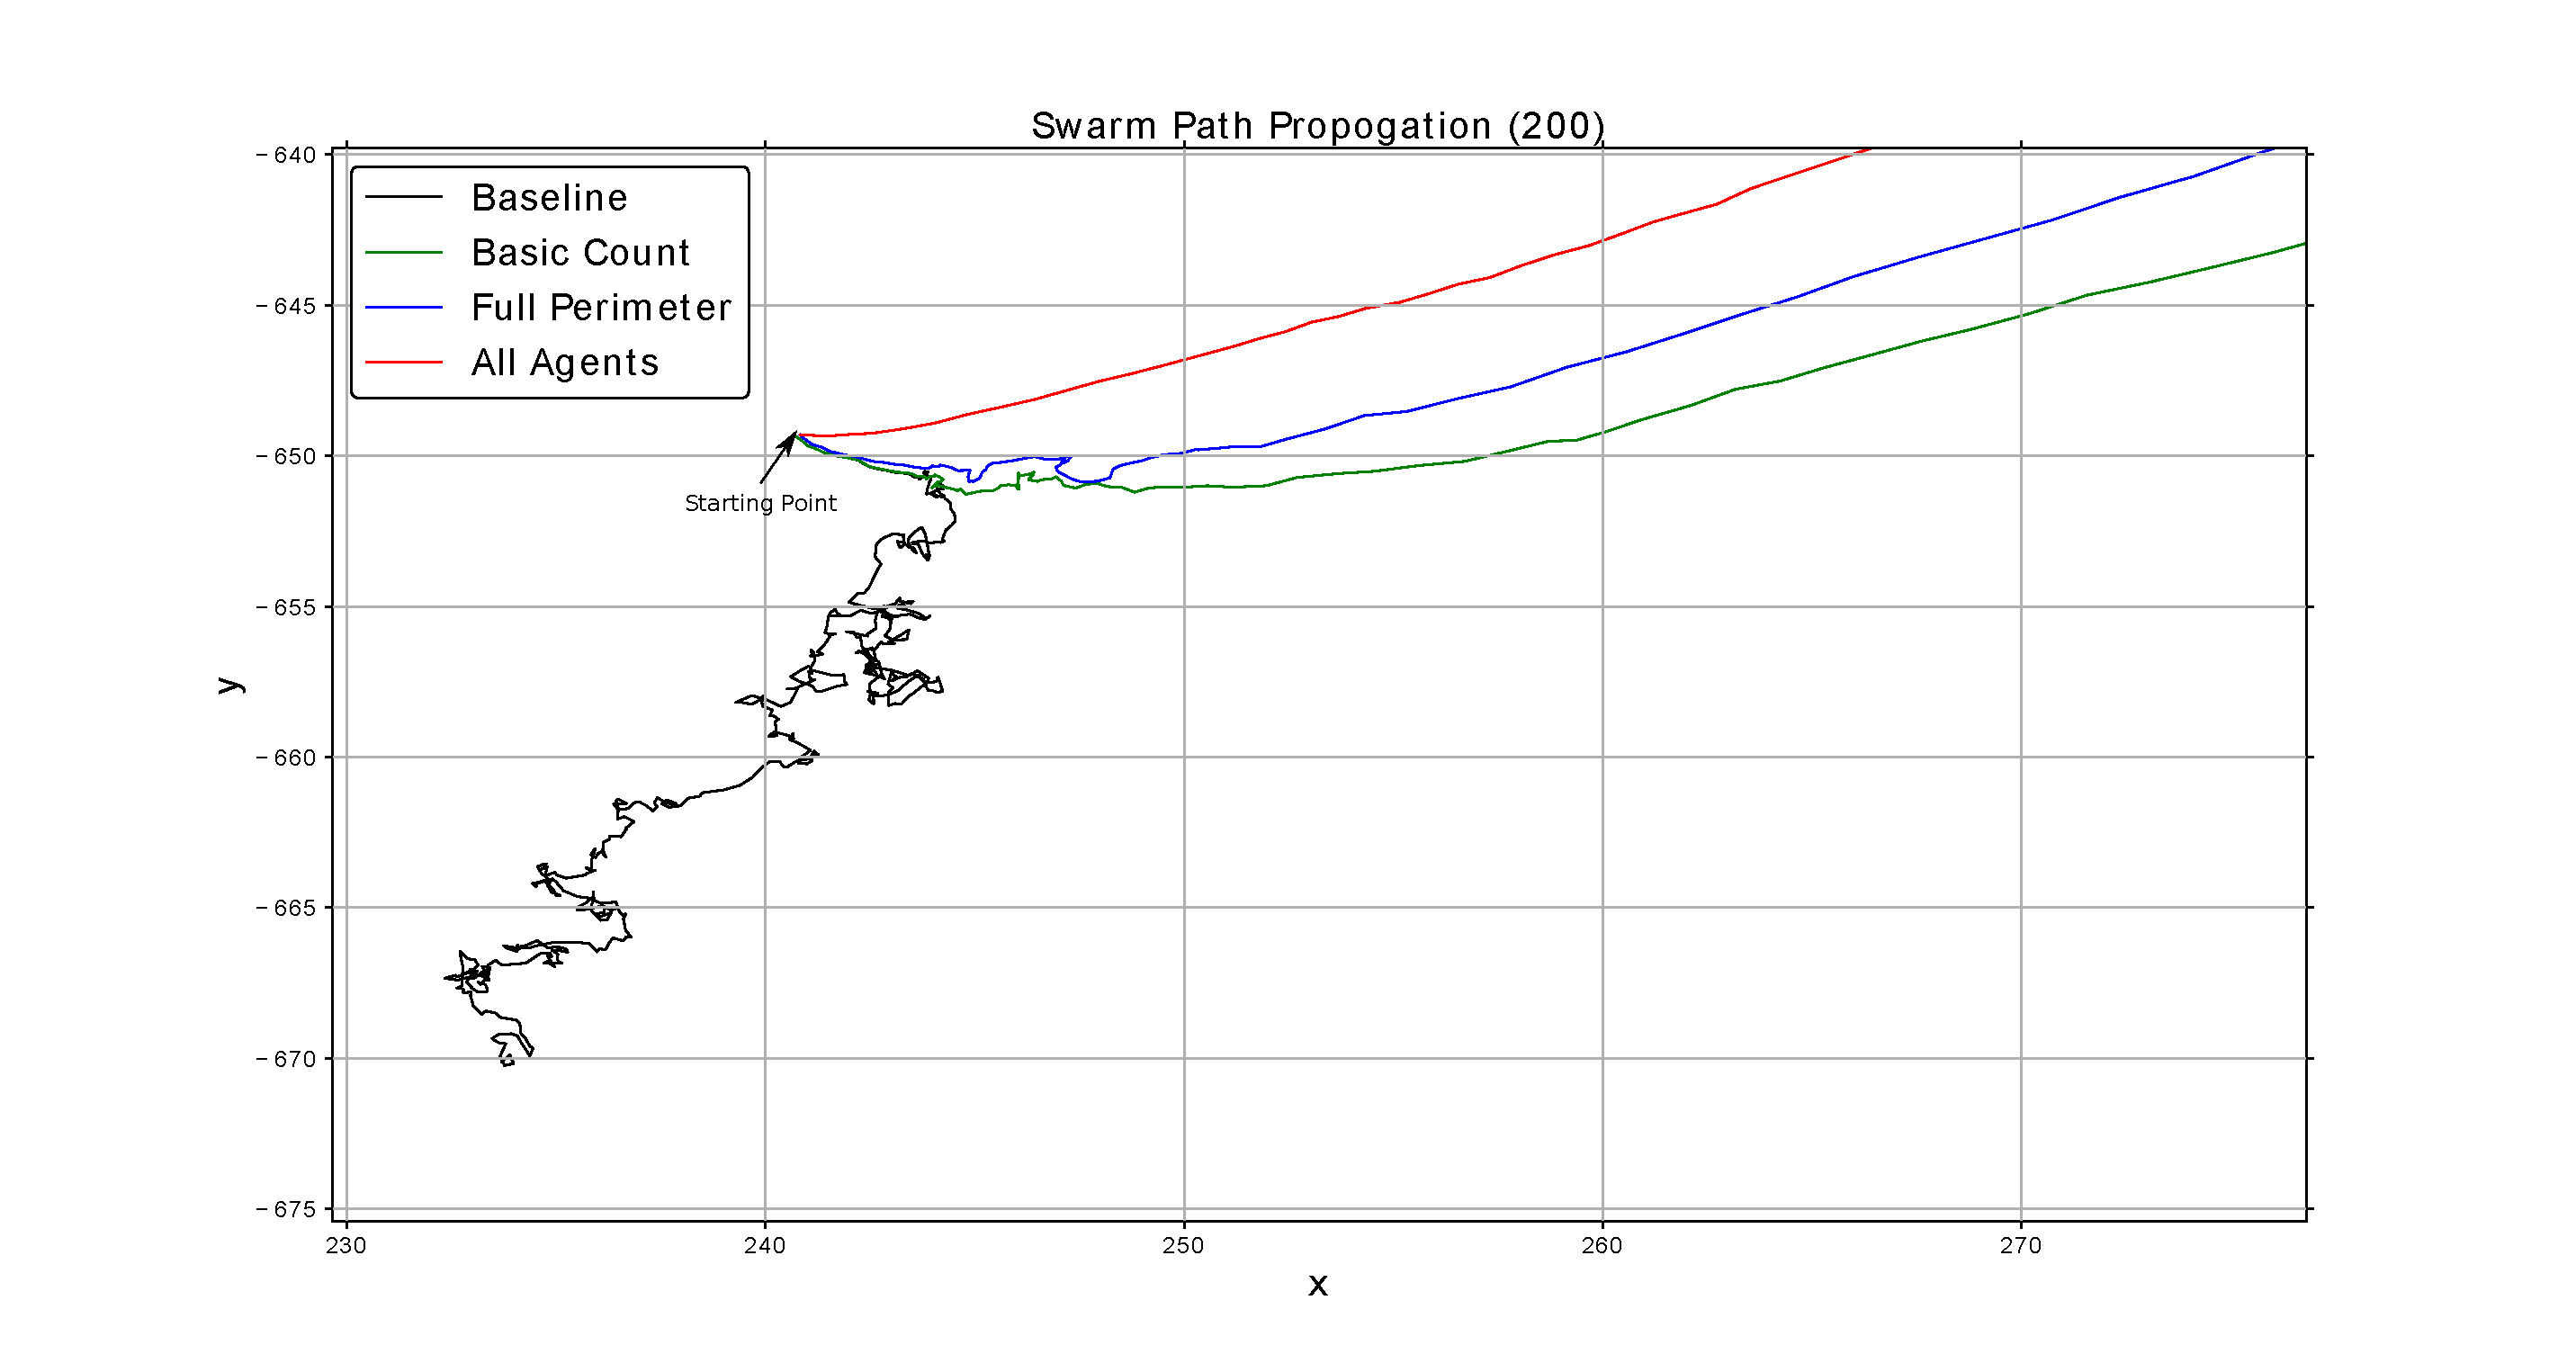
\includegraphics[width=14cm]{CHAPTER-6/figures/SwarmPropagationComparison1}
\end{center}
\caption{Swarm propagation path comparison\label{reduced:SwarmPropagationPathComparison1}}
\end{figure}

Figure~\ref{reduced:SwarmPropagationPathComparison1} shows the initial expansion phase of the swarm from deployment. Figure~\ref{reduced:SwarmPropagationPathComparison2} shows the paths for the full simulation runs and the baseline comparison.

\begin{figure}[H]
\begin{center}
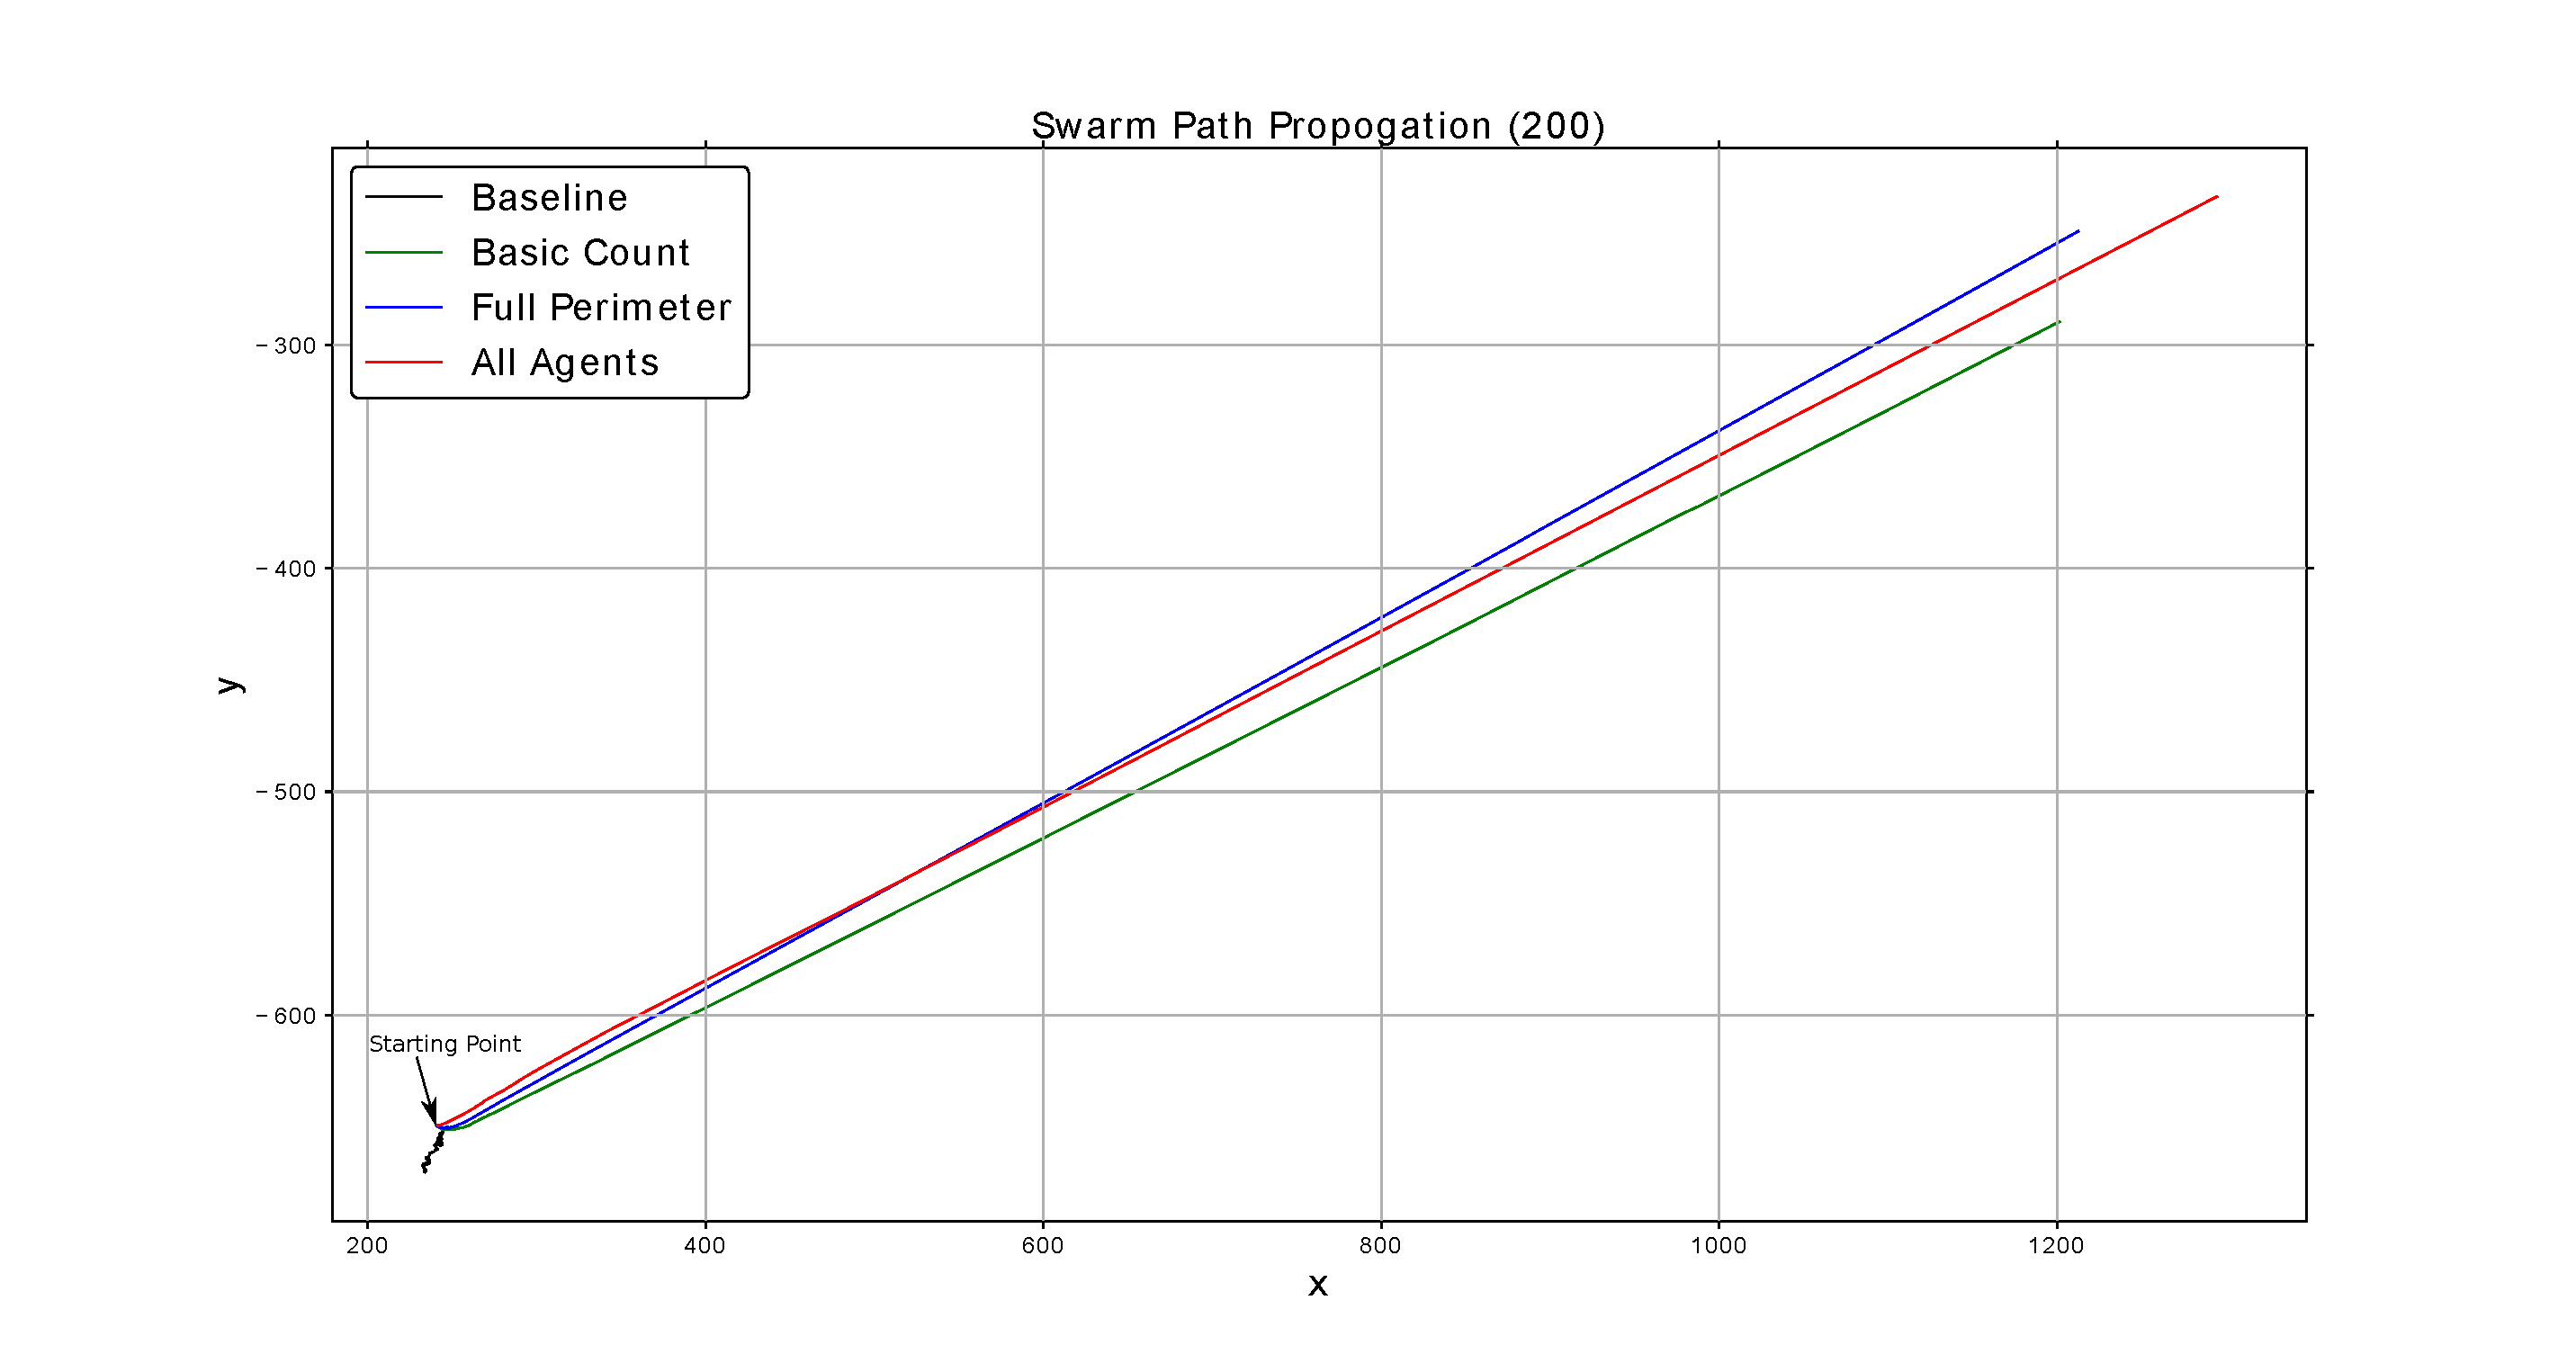
\includegraphics[width=14cm]{CHAPTER-6/figures/SwarmPropagationComparison2}
\end{center}
\caption{Swarm propagation path comparison\label{reduced:SwarmPropagationPathComparison2}}
\end{figure}

Using all agents as coordinators results in the swarm immediately moving in the direction of the destination. The full perimeter detection has a limited effect on the direction of travel until the internal vectors start to balance and the internal magnitudes can be affected by a \textit{destination vectors} at which point the swarm travels in the direction of the destination. The basic-count algorithm stabilises and then moves towards the destination in a similar manner to the full perimeter except in the initial compressed disorganised stage the basic-count algorithm develops in the same manner as the baseline swarm where there are no coordinators. These experimental results demonstrate that reducing the GPS utilisation has two effects on the swarm's propagation. Firstly it is possible to reduce the number of GPS sensors required to coordinate a swarm and it is possible to manage the `jitter' while applying a directional bias on a swarm using \textit{destination vectors}. 

The effect of the algorithms on the stabilisation period can be seen in~figure~\ref{reduced:SwarmPropagationPathComparison3} which shows the swarm paths at the end of the 60 seconds simulation period. The relative positions shows the distances that the swarm is able to travel while employing the three algorithms, this is based on the swarm centroid. The baseline centroid path shows that without a \textit{destination vector} being applied the swarm's centroid moves but it is based upon the \textit{interaction vectors} only and there is no directional bias.

\begin{figure}[H]
\begin{center}
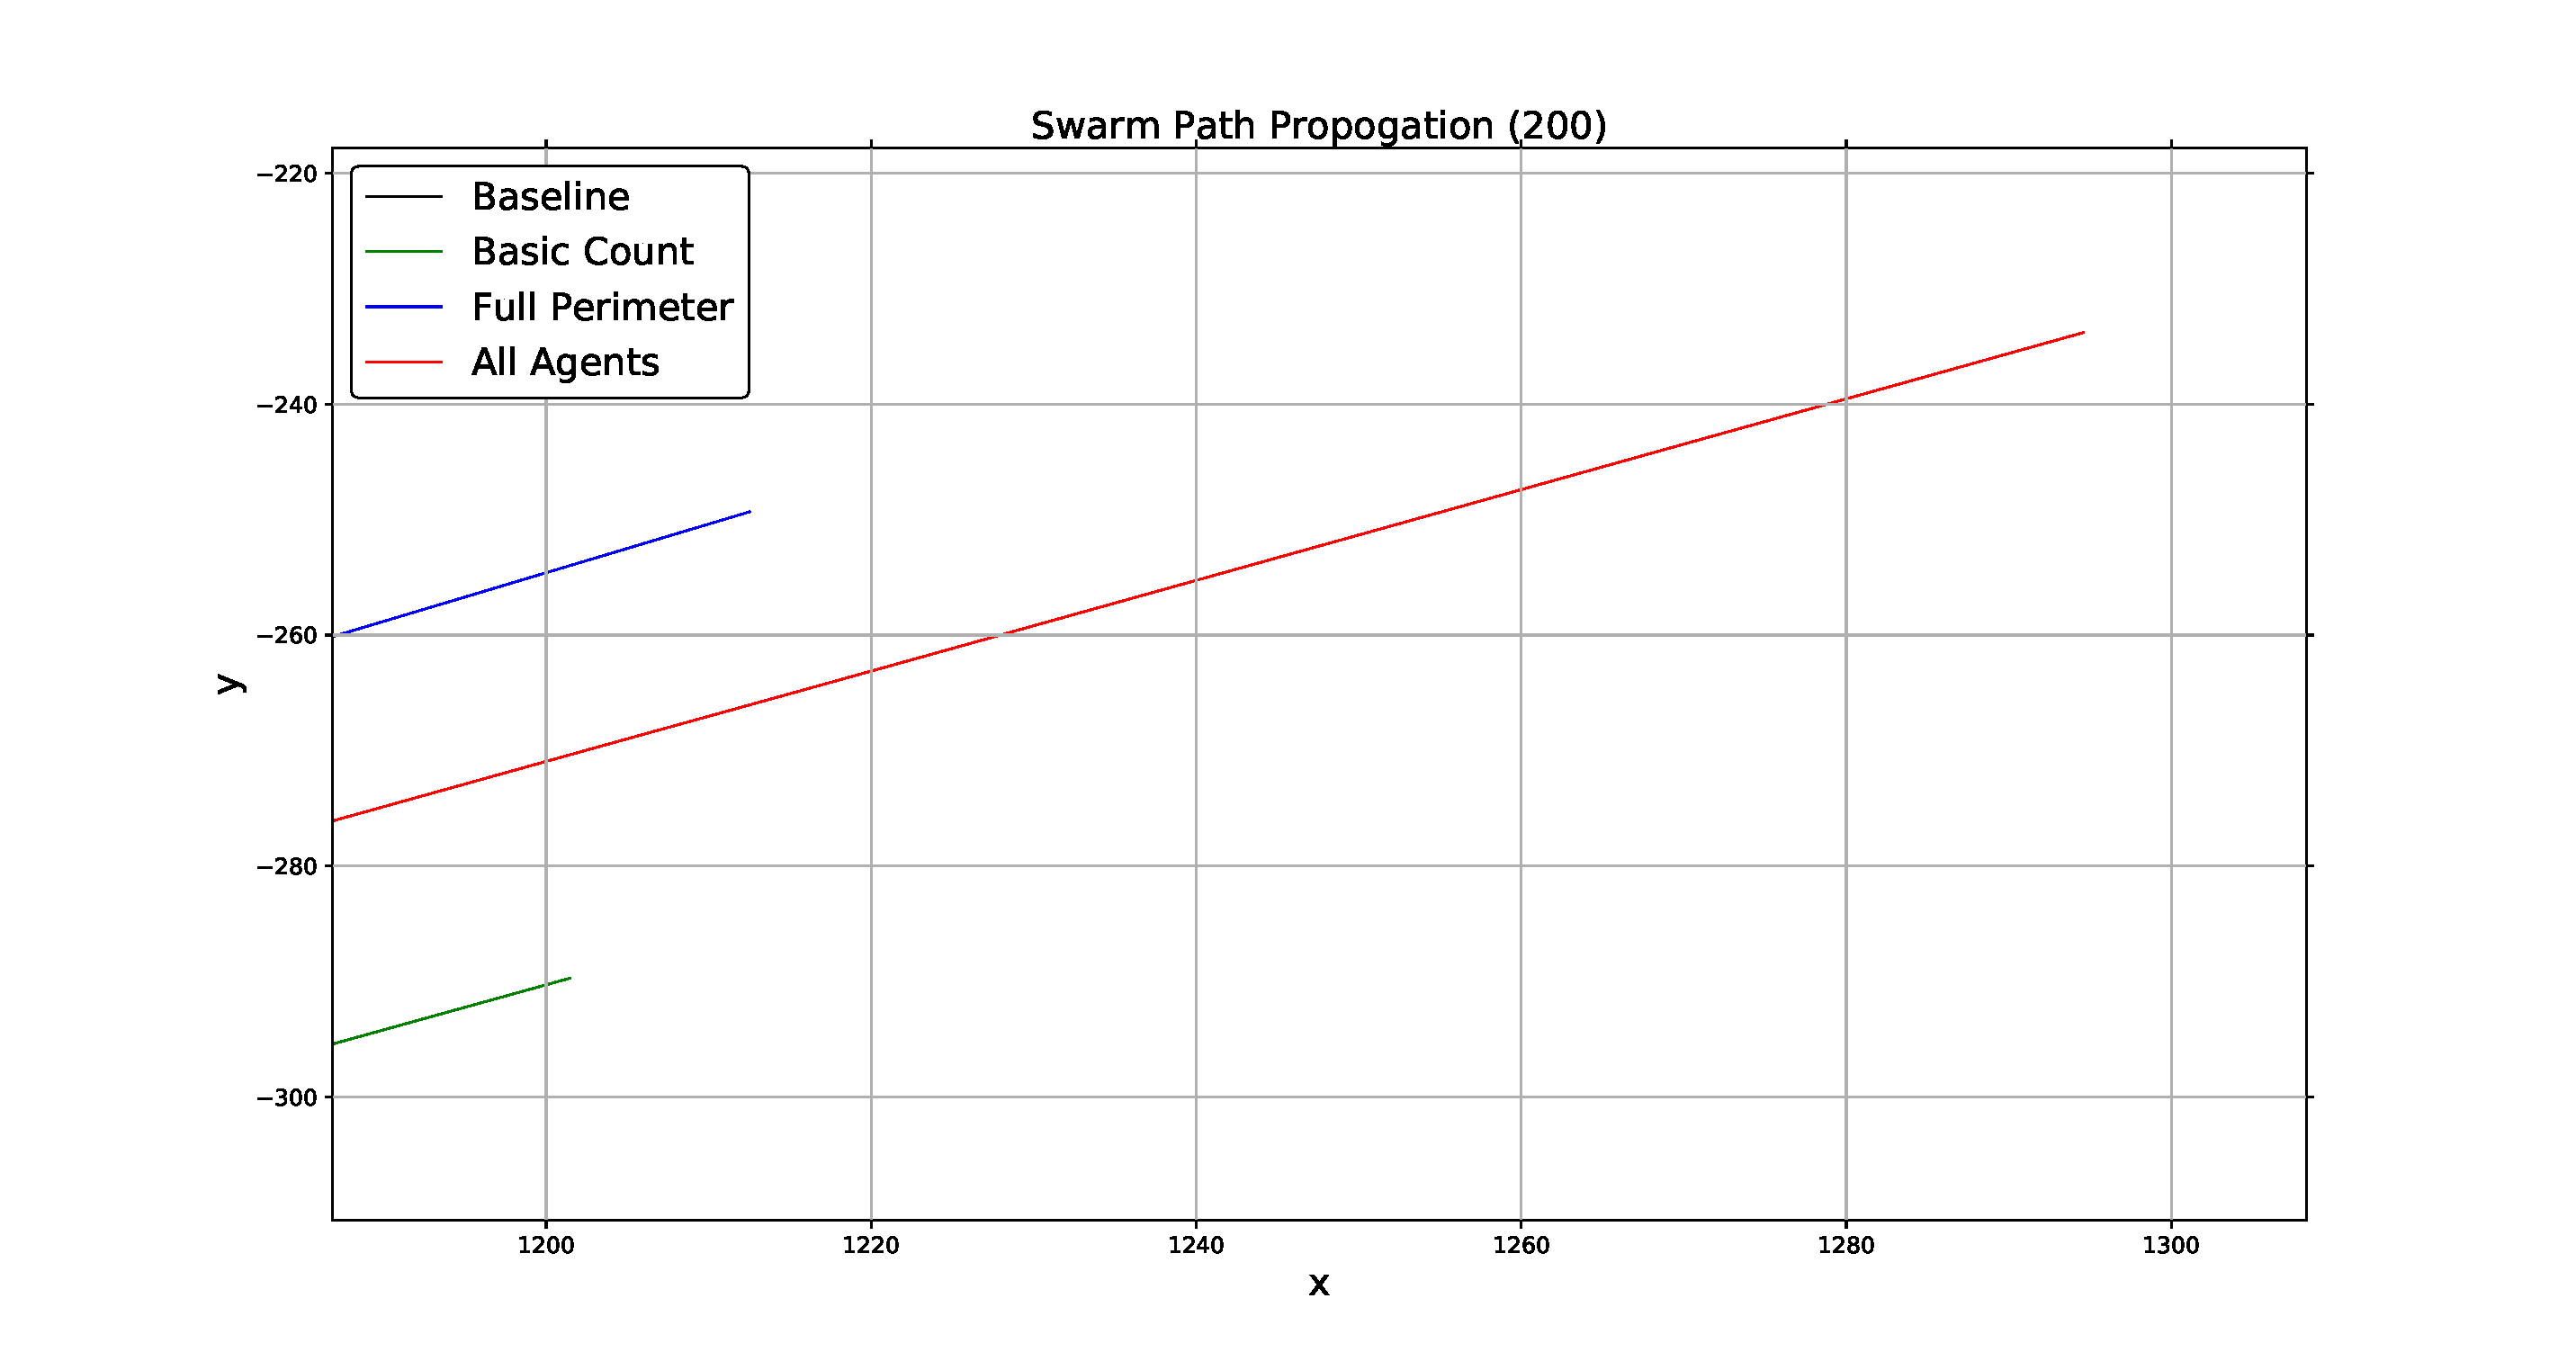
\includegraphics[width=14cm]{CHAPTER-6/figures/SwarmPropagationComparison3}
\end{center}
\caption{Swarm traversal at end of 60s run\label{reduced:SwarmPropagationPathComparison3}}
\end{figure}

\subsection{Speed of Swarm (Based on centroid)}
To determine the speed a swarm is travelling a single reference point needs to be identified. A swarm's speed is measured based upon the position of its centroid, as discussed by Gazi and Passino~\cite{GP:04, GP:02}.

The speed at which the swarm travels is calculated as the distance the centroid moves~(Equation~\ref{eq:SwarmDistance1}) over a set time~(Equation~\ref{eq:SwarmSpeed1}). Equation~\ref{eq:SwarmDistance1} shows the formulae for the distance a swarm has travelled over a set period of time, $t \rightarrow t^{1}$ where $d$ is the distance the centroid has travelled, $x,y$ is the centroid of the swarm and $t$ is time.

\begin{equation}\label{eq:SwarmDistance1}
d = \sqrt{(x_{t}-x_{t^1})^2+(y_{t}-y_{t^1})^2}
\end{equation}‎

\begin{equation}\label{eq:SwarmSpeed1}
S_s = \frac{d}{n}
\end{equation}‎

Equation~\ref{eq:SwarmSpeed1} shows how the speed is calculated based on the distance in equation~\ref{eq:SwarmDistance1}. $S_s$ is the speed of the swarm's centroid and $n$ is the number of time increments.

Once the swarm has stabilised it migrates towards the destination. Each of the algorithms has an effect on how many coordinators are used to control the direction of the swarm~(Figure~\ref{fig:SwarmPerimeter1}). The impact of the number of coordinators is expected to affect the propagation speed of the swarm towards its destination. Based upon the final positions of the swarms over the last 20 seconds of their simulations it is shown that there was only a marginal impact on the speed of the swarm once stabilised~(Figure~\ref{fig:SwarmSpeed1}). The difference in the algorithms only affects the time it takes the swarm to stabilise to the level that the \textit{destination vectors} can influence the swarm's movement.

The results also show a reduction in energy usage (GPS usage) is possible with minimal effect on the overall speed of the swarm (taken from the centroid). 

Although the agents within the swarm have travelled the same distances the overall path of the swarms has been affected~(Table~\ref{tab:SwarmSpeed2}).

The time frame for the results in~table~\ref{tab:SwarmSpeed1},~\ref{tab:SwarmSpeed2},~\ref{tab:SwarmSpeed3} are for a time slice from 40~-~60~seconds in the simulation.

\begin{table}[H]
\begin{center}
\begin{tabular}{| l | l |}
\hline
GPS Model & Start \\ \hline
All-agents & (922.5254184933, 379.965865509344) \\ \hline
Basic-count & (828.5991571583, 433.5750489635) \\ \hline
Full perimeter & (848.1131820415, 410.9739402922) \\ \hline
\end{tabular}\caption{Swarm centroid after stabilisation (40s)} \label{tab:SwarmSpeed1}
\end{center}
\end{table}

\begin{table}[H]
\begin{center}
\begin{tabular}{| l | l |}
\hline
GPS Model & End  \\ \hline
All-agents & (1294.5940641812, 233.788749492987) \\ \hline
Basic-count & (1201.4534856023, 289.7373900729) \\ \hline
Full perimeter & (1218.1290381962, 260.3440891182)\\ \hline
\end{tabular}\caption{Swarm centroid after stabilisation (60s)} \label{tab:SwarmSpeed2}
\end{center}
\end{table}

\begin{table}[H]
\begin{center}
\begin{tabular}{| l | l | l |}
\hline
GPS Model & Distance & Speed \\ \hline
All-agents &  399.7534569593 & 19.987672848 \\  \hline
Basic-count & 399.6368631077 & 19.9818431554 \\ \hline
Full perimeter & 399.5010461444 & 19.9750523072 \\  \hline
\end{tabular}\caption{Swarm distance and speed after stabilisation (40s-60s)} \label{tab:SwarmSpeed3}
\end{center}
\end{table}

\begin{table}[H]
\begin{center}
\begin{tabular}{| l | l | l |}
\hline
GPS Model & End & Distance \\ \hline
All-agents & (1294.5940641812, 233.788749492987) & 588.5813143506\\ \hline
Basic-count & (1201.4534856023, 289.7373900729) & 696.0606134399\\ \hline
Full Perimeter & (1218.1290381962, 260.3440891182) & 669.4489951522\\ \hline
\end{tabular}\caption[Distance to destination after run]{Distance to destination after run \textit{(end = [1841,15])}}\label{tab:SwarmDistanceEnd}
\end{center}
\end{table}

\begin{figure}[H]
\begin{center}
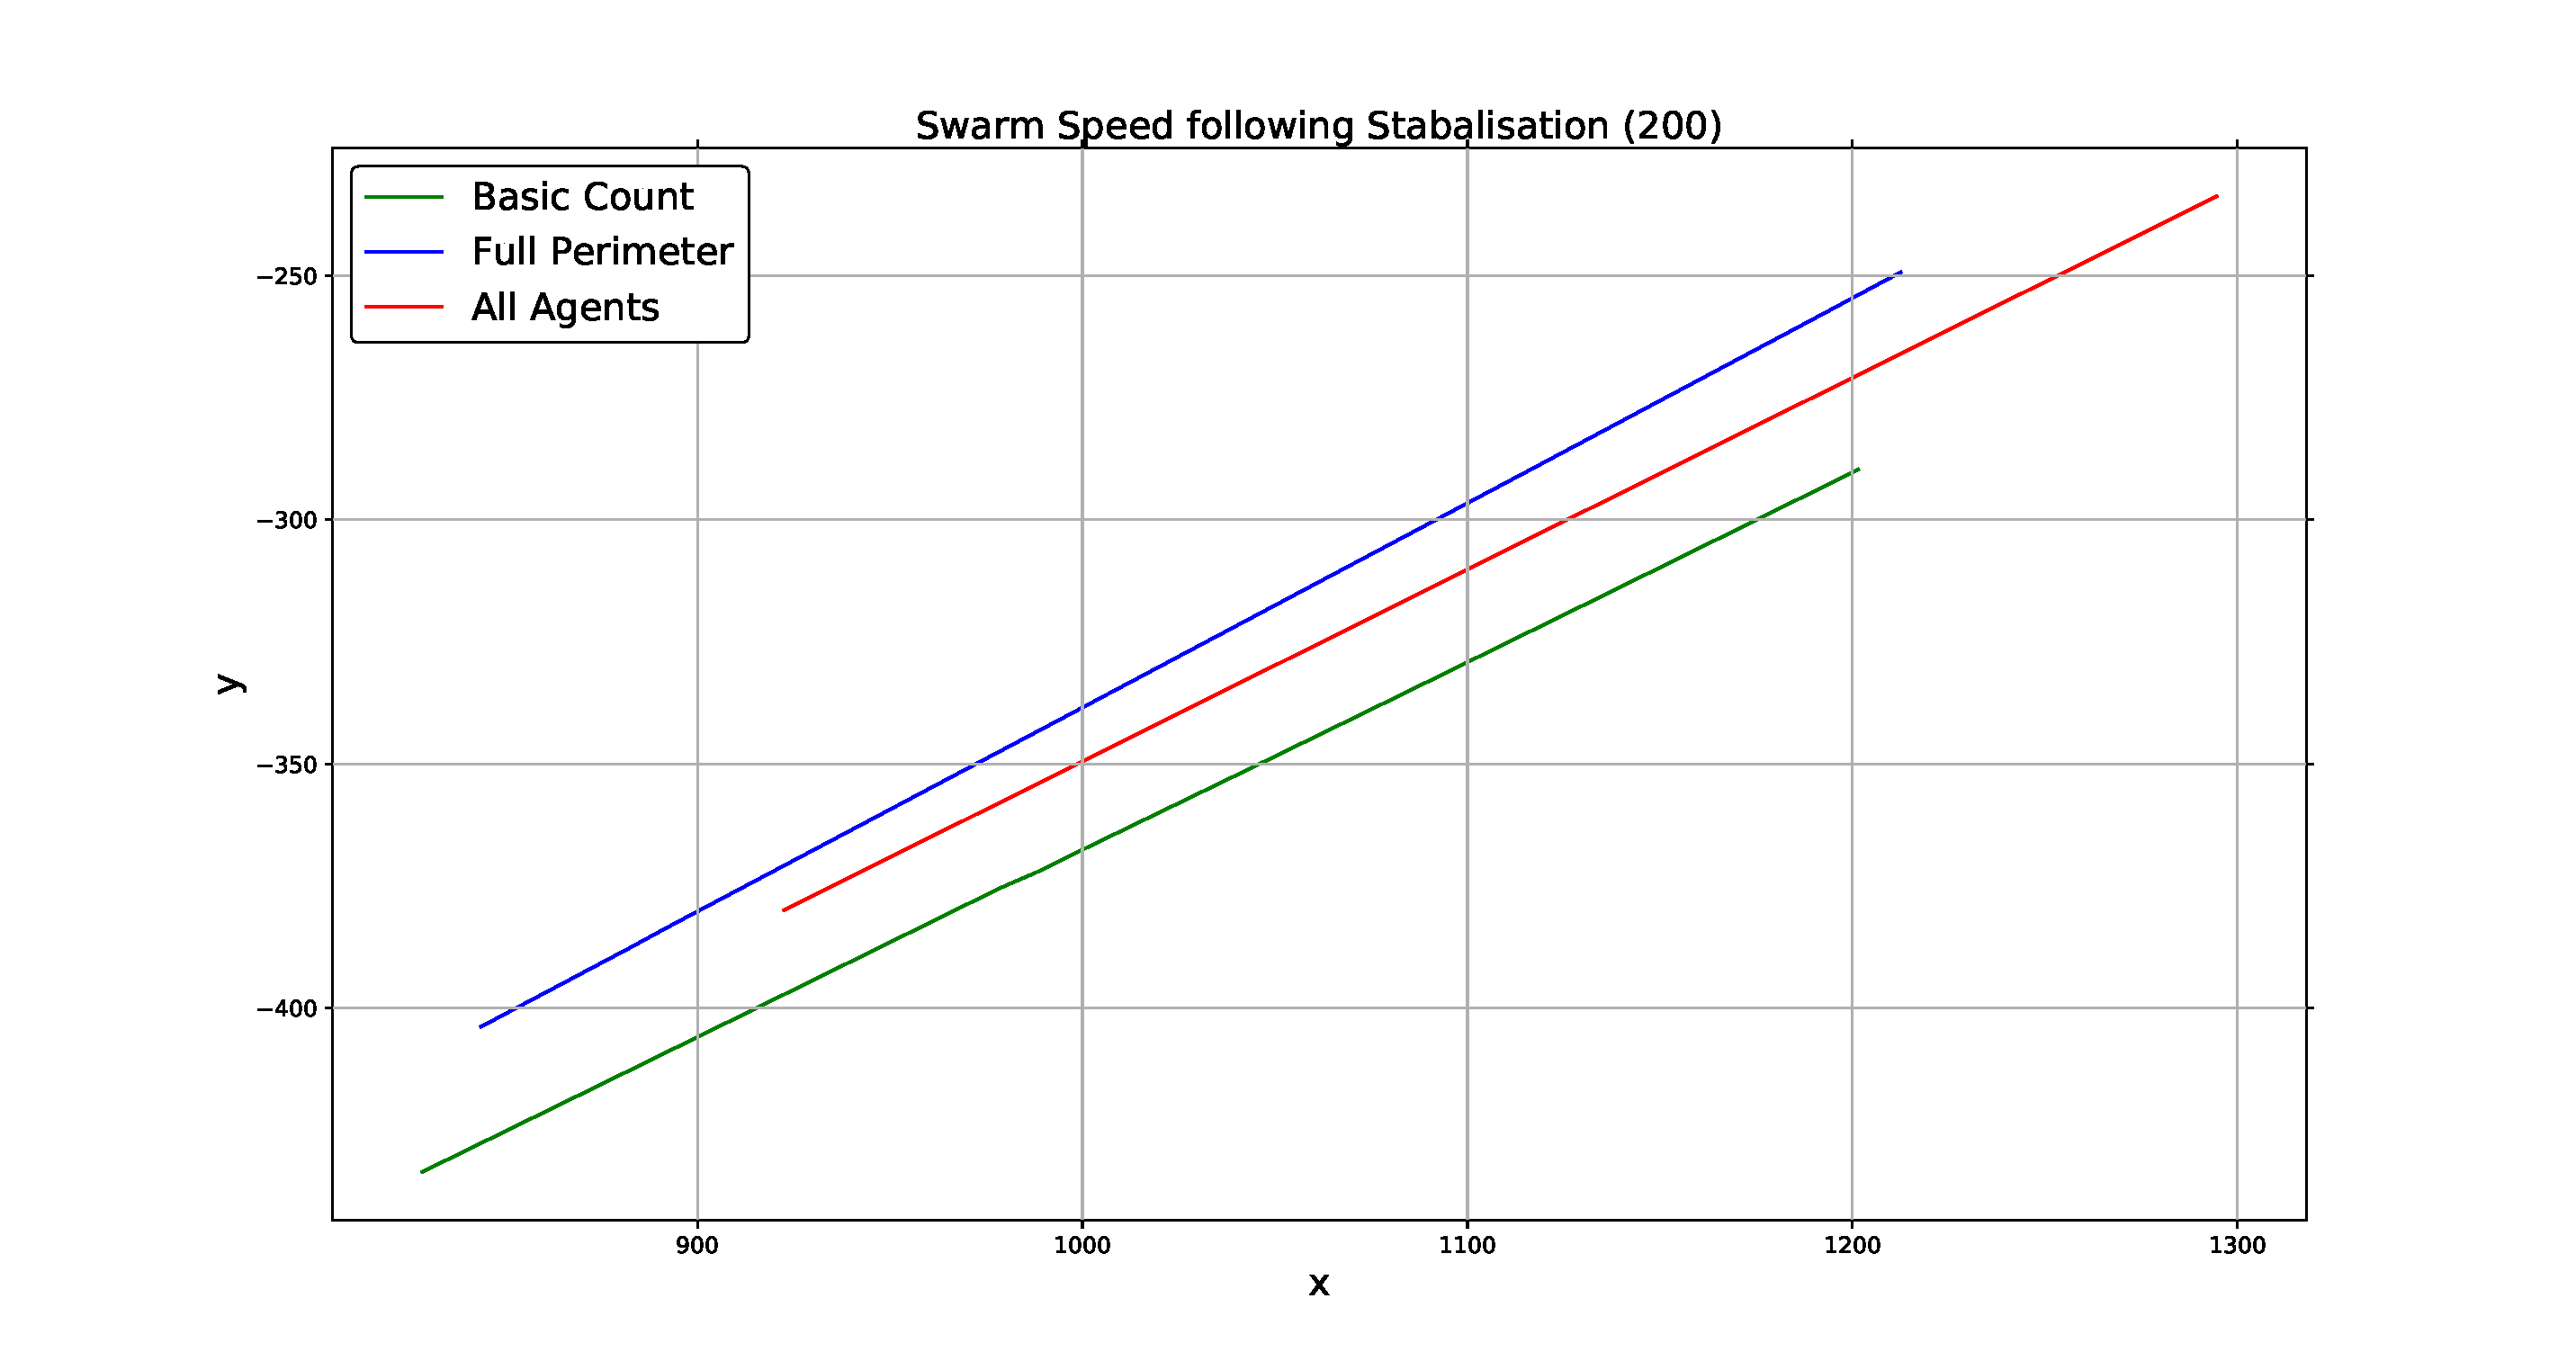
\includegraphics[width=14cm]{CHAPTER-6/figures/SwarmSpeed1}
\end{center}
\caption{200 agent swarm path (over 20s period)\label{fig:SwarmSpeed1}}
\end{figure}

\subsection{Alternate weightings for directional bias}\label{sec:AlternateBias1}
The overall effect of the directional bias is affected by the number of coordinator agents in a swarm. Increasing the bias affects the jitter therefore balancing the weighting should have a positive effect in reducing the jitter.

The impact of the bias can be seen in the effect it has upon the number of neighbours an agent has during the path propagation.

\begin{figure}[H]
\begin{center}
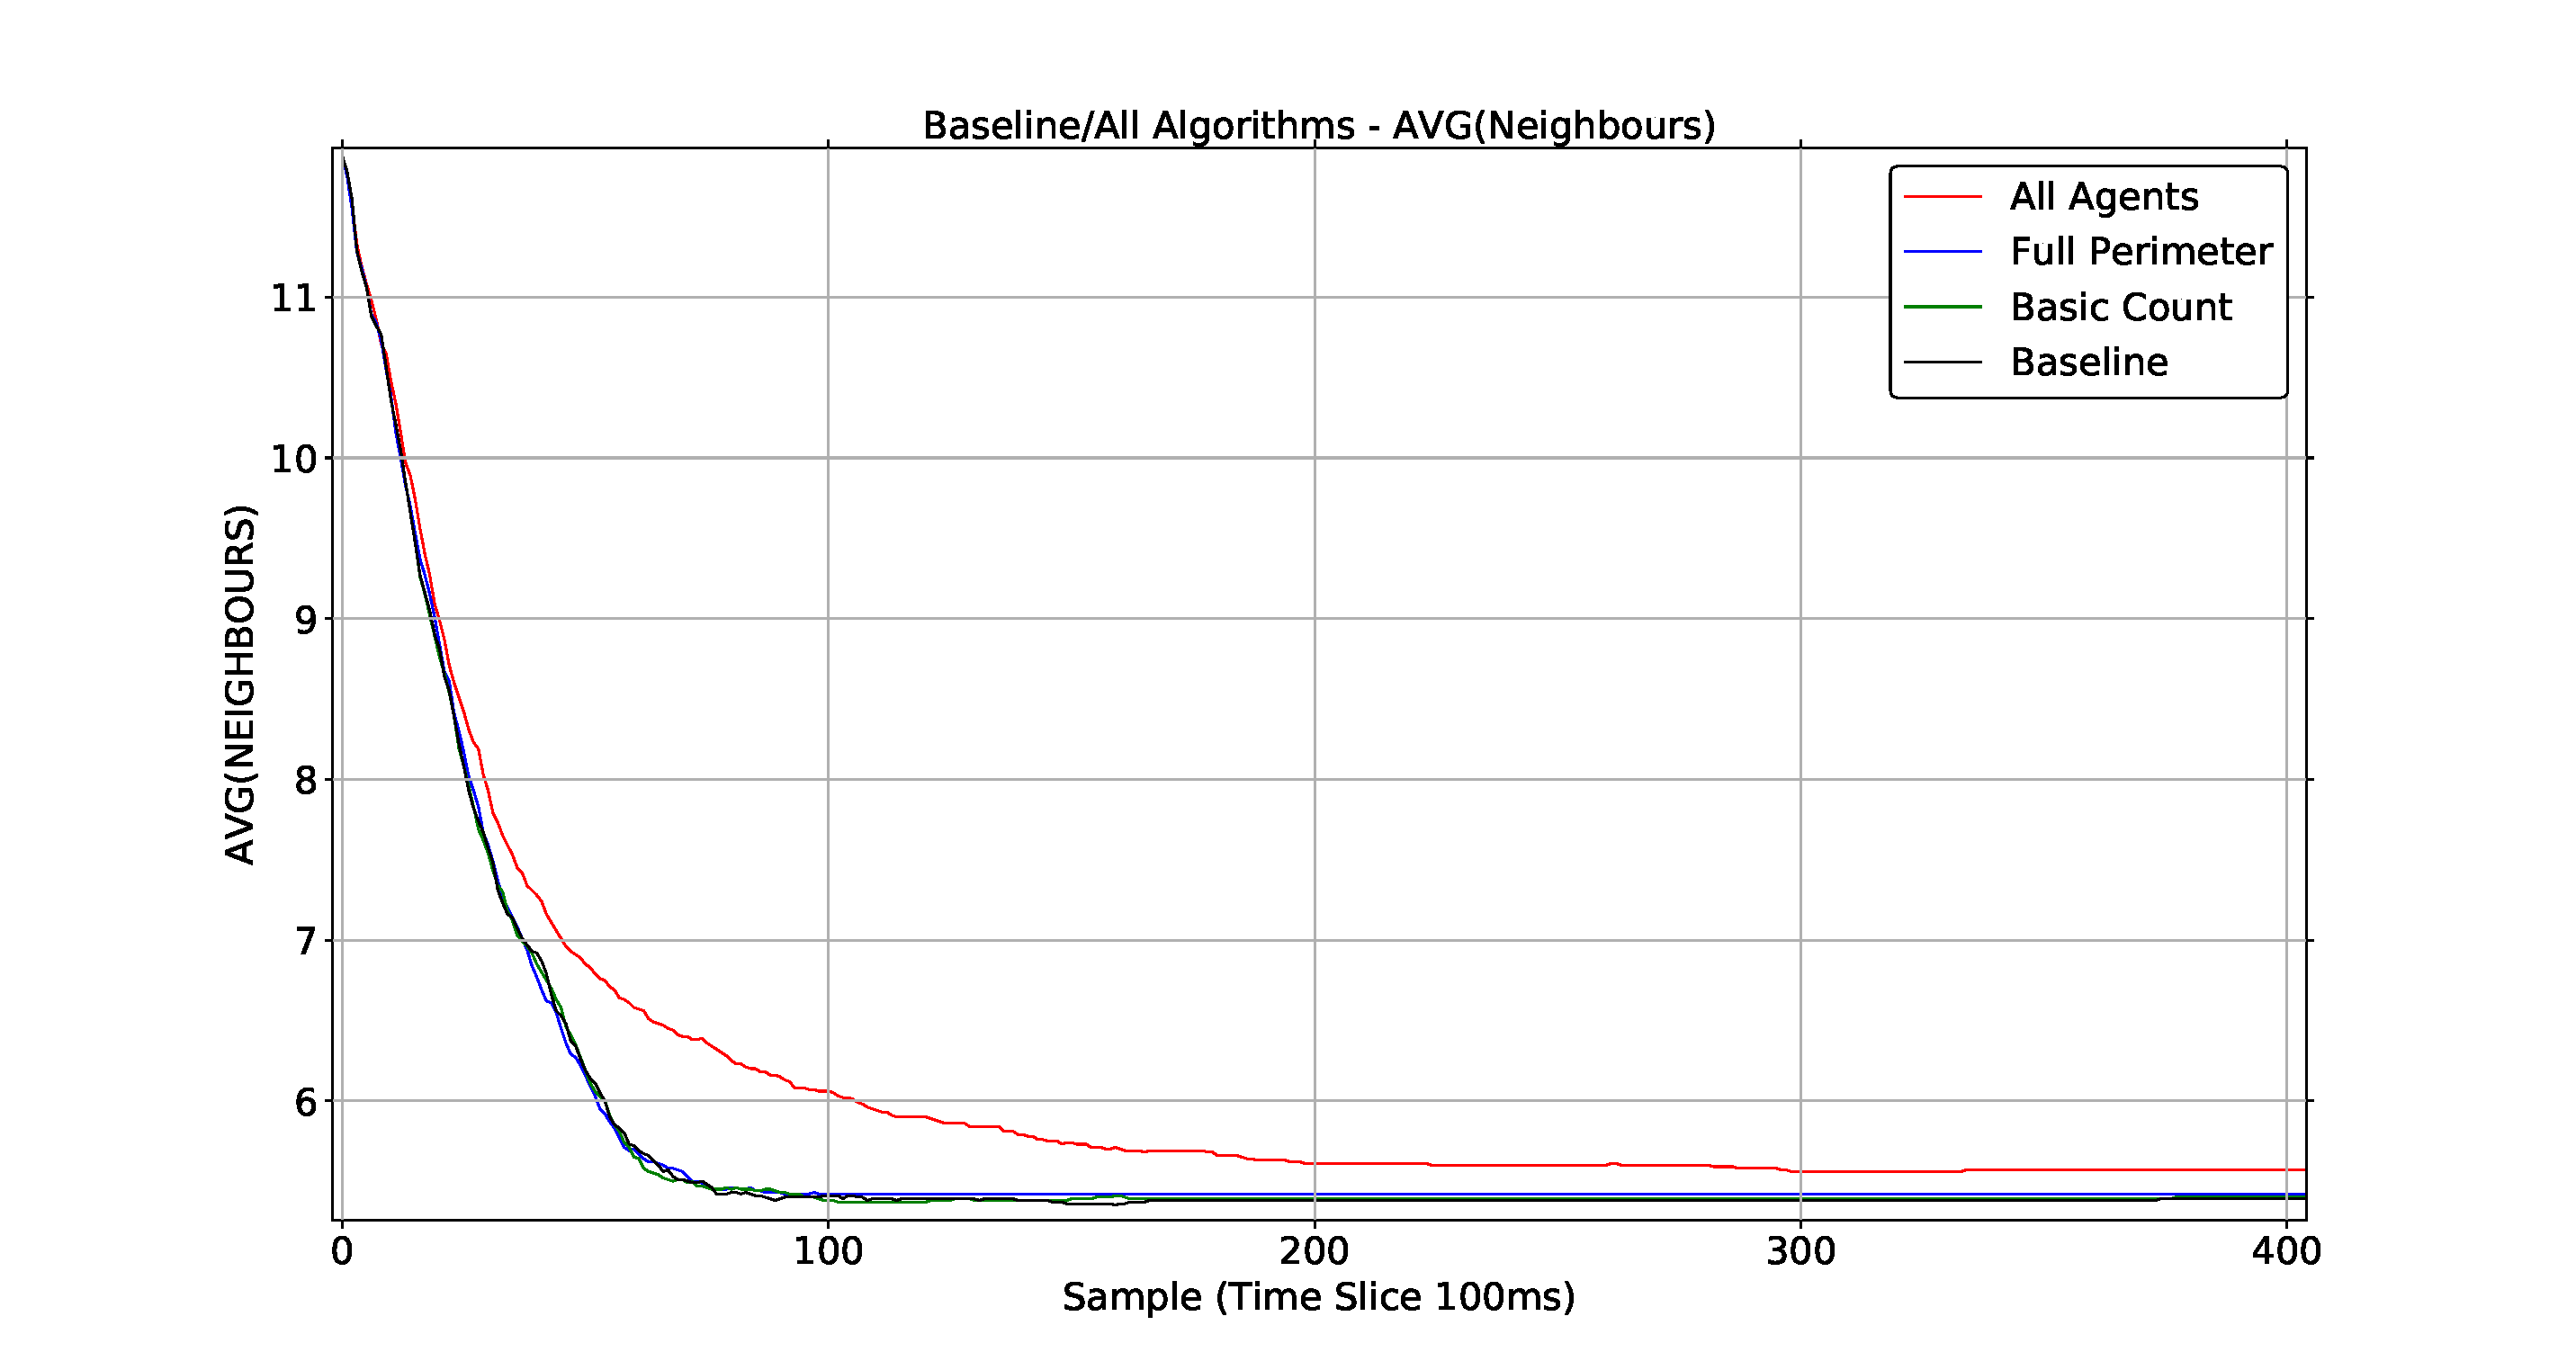
\includegraphics[width=14cm]{CHAPTER-6/figures/SwarmNeighbourCount}
\end{center}
\caption{Neighbour count effect from \textit{destination vectors}\label{fig:SwarmNeighbourCount}}
\end{figure}

Figure~\ref{fig:SwarmNeighbourCount} shows that for each of the algorithms the lattice effect (determined by neighbour count) takes longer to settle the more coordinators there are. In the case of the `all agent' coordinated swarm the agents are affected most significantly and therefore exhibit the high variation in magnitudes and distances.

The coordinator statistics demonstrates~(Table~\ref{tab:GPSUsage}) the weighting of the \textit{destination vectors} can be adjusted to produce an overall effect that is similar for each algorithm. If the weightings are adjusted taking the basic-count as the baseline goal-based swarm then the `all agents' and `full perimeter' algorithms can be weighted proportionally such that they have an overall \textit{direction vector magnitude} that is similar to the basic-count~table~\ref{tab:GPSWeighting}. The effects of this is shown in Figures~\ref{fig:BaselineAll100-60-20-1}, \ref{fig:BaselineAllMag100-60-20-1}, and \ref{fig:SwarmNeighbourCountBalanced}

\begin{table}[H]
\begin{center}
\begin{tabular}{| l | c | c | l |}
\hline
GPS Model & Bots GPS & \% Usage & Weighting \\ \hline
All-agents & 200 & 100\% & 20 \\ \hline
Basic-count & 40 & 20\% & 100 \\ \hline
Full perimeter & 72 & 36\% & 60 \\  \hline
\end{tabular}\caption{Swarm GPS proportional weighting}\label{tab:GPSWeighting}
\end{center}
\end{table}

\begin{figure}[H]
\begin{center}
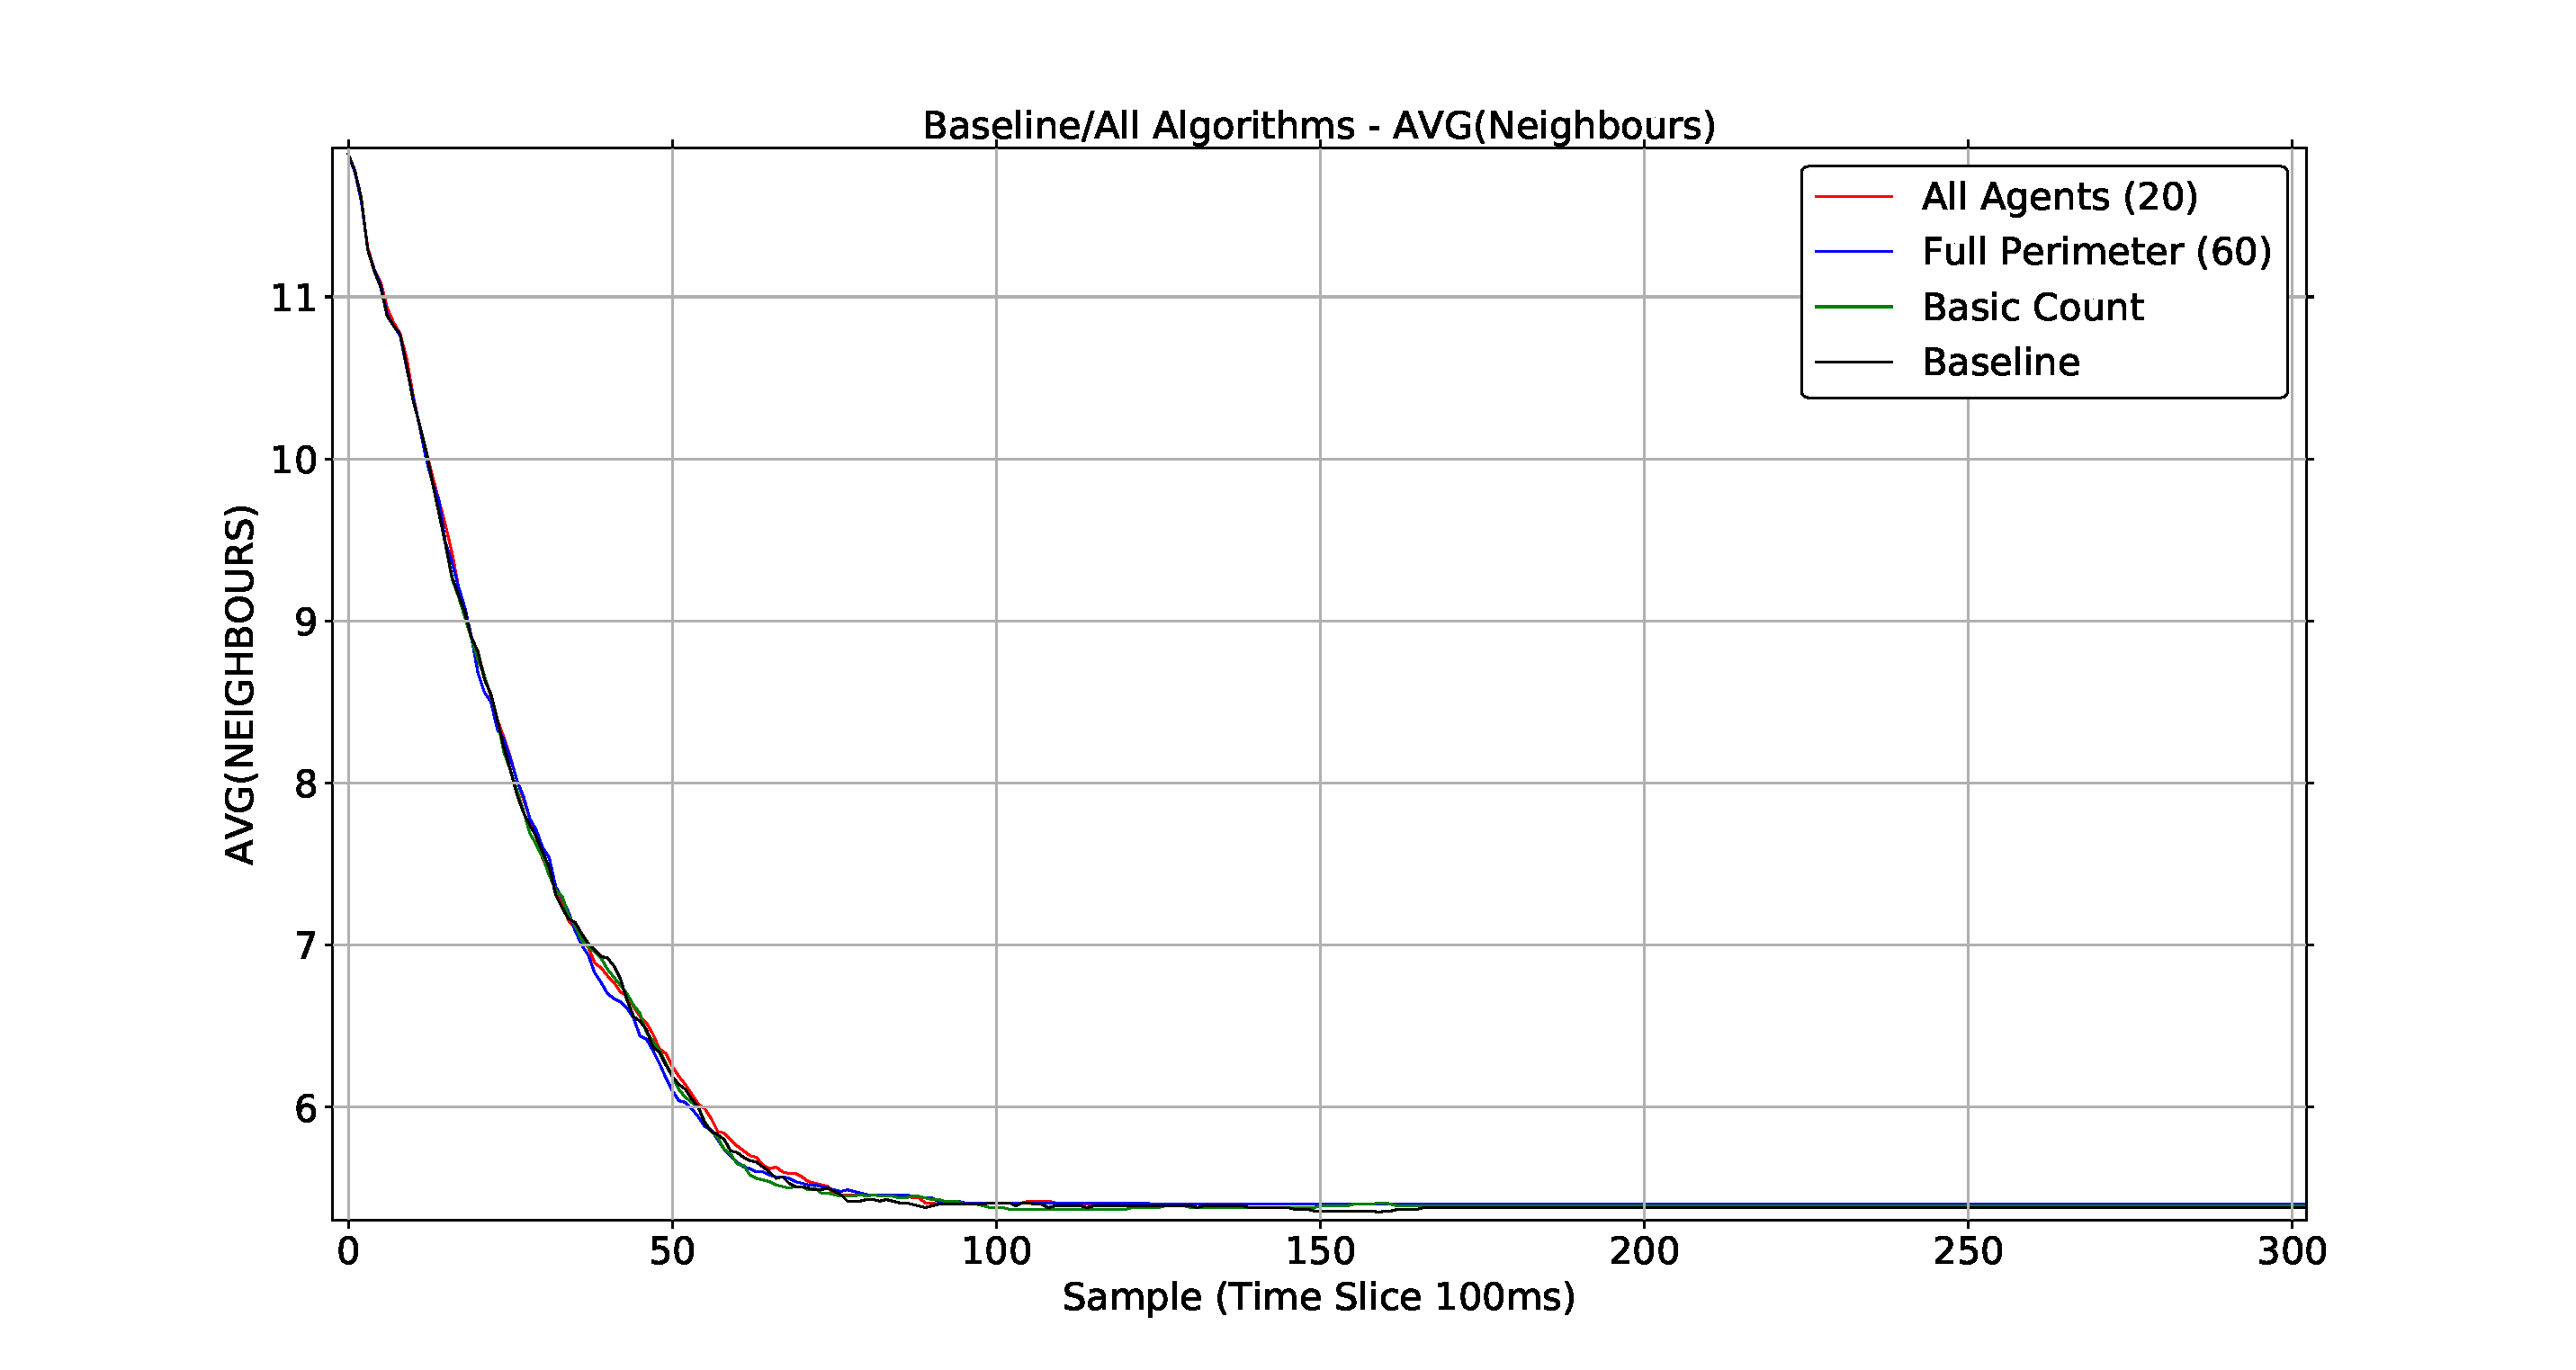
\includegraphics[width=14cm]{CHAPTER-6/figures/SwarmNeighbourCountBalanced}
\end{center}
\caption{Neighbour count effect from balanced directional bias\label{fig:SwarmNeighbourCountBalanced}}
\end{figure}

Figure~\ref{fig:SwarmNeighbourCountBalanced} shows the effect reducing the \textit{destination vector magnitude} has on the swarm structure. The reduction brings the stability (jitter) of the three algorithms in line such that all the algorithms have a similar impact on the swarm producing swarms with more stable structures while still creating a goal based affect. 

\begin{figure}[H]
\begin{center}
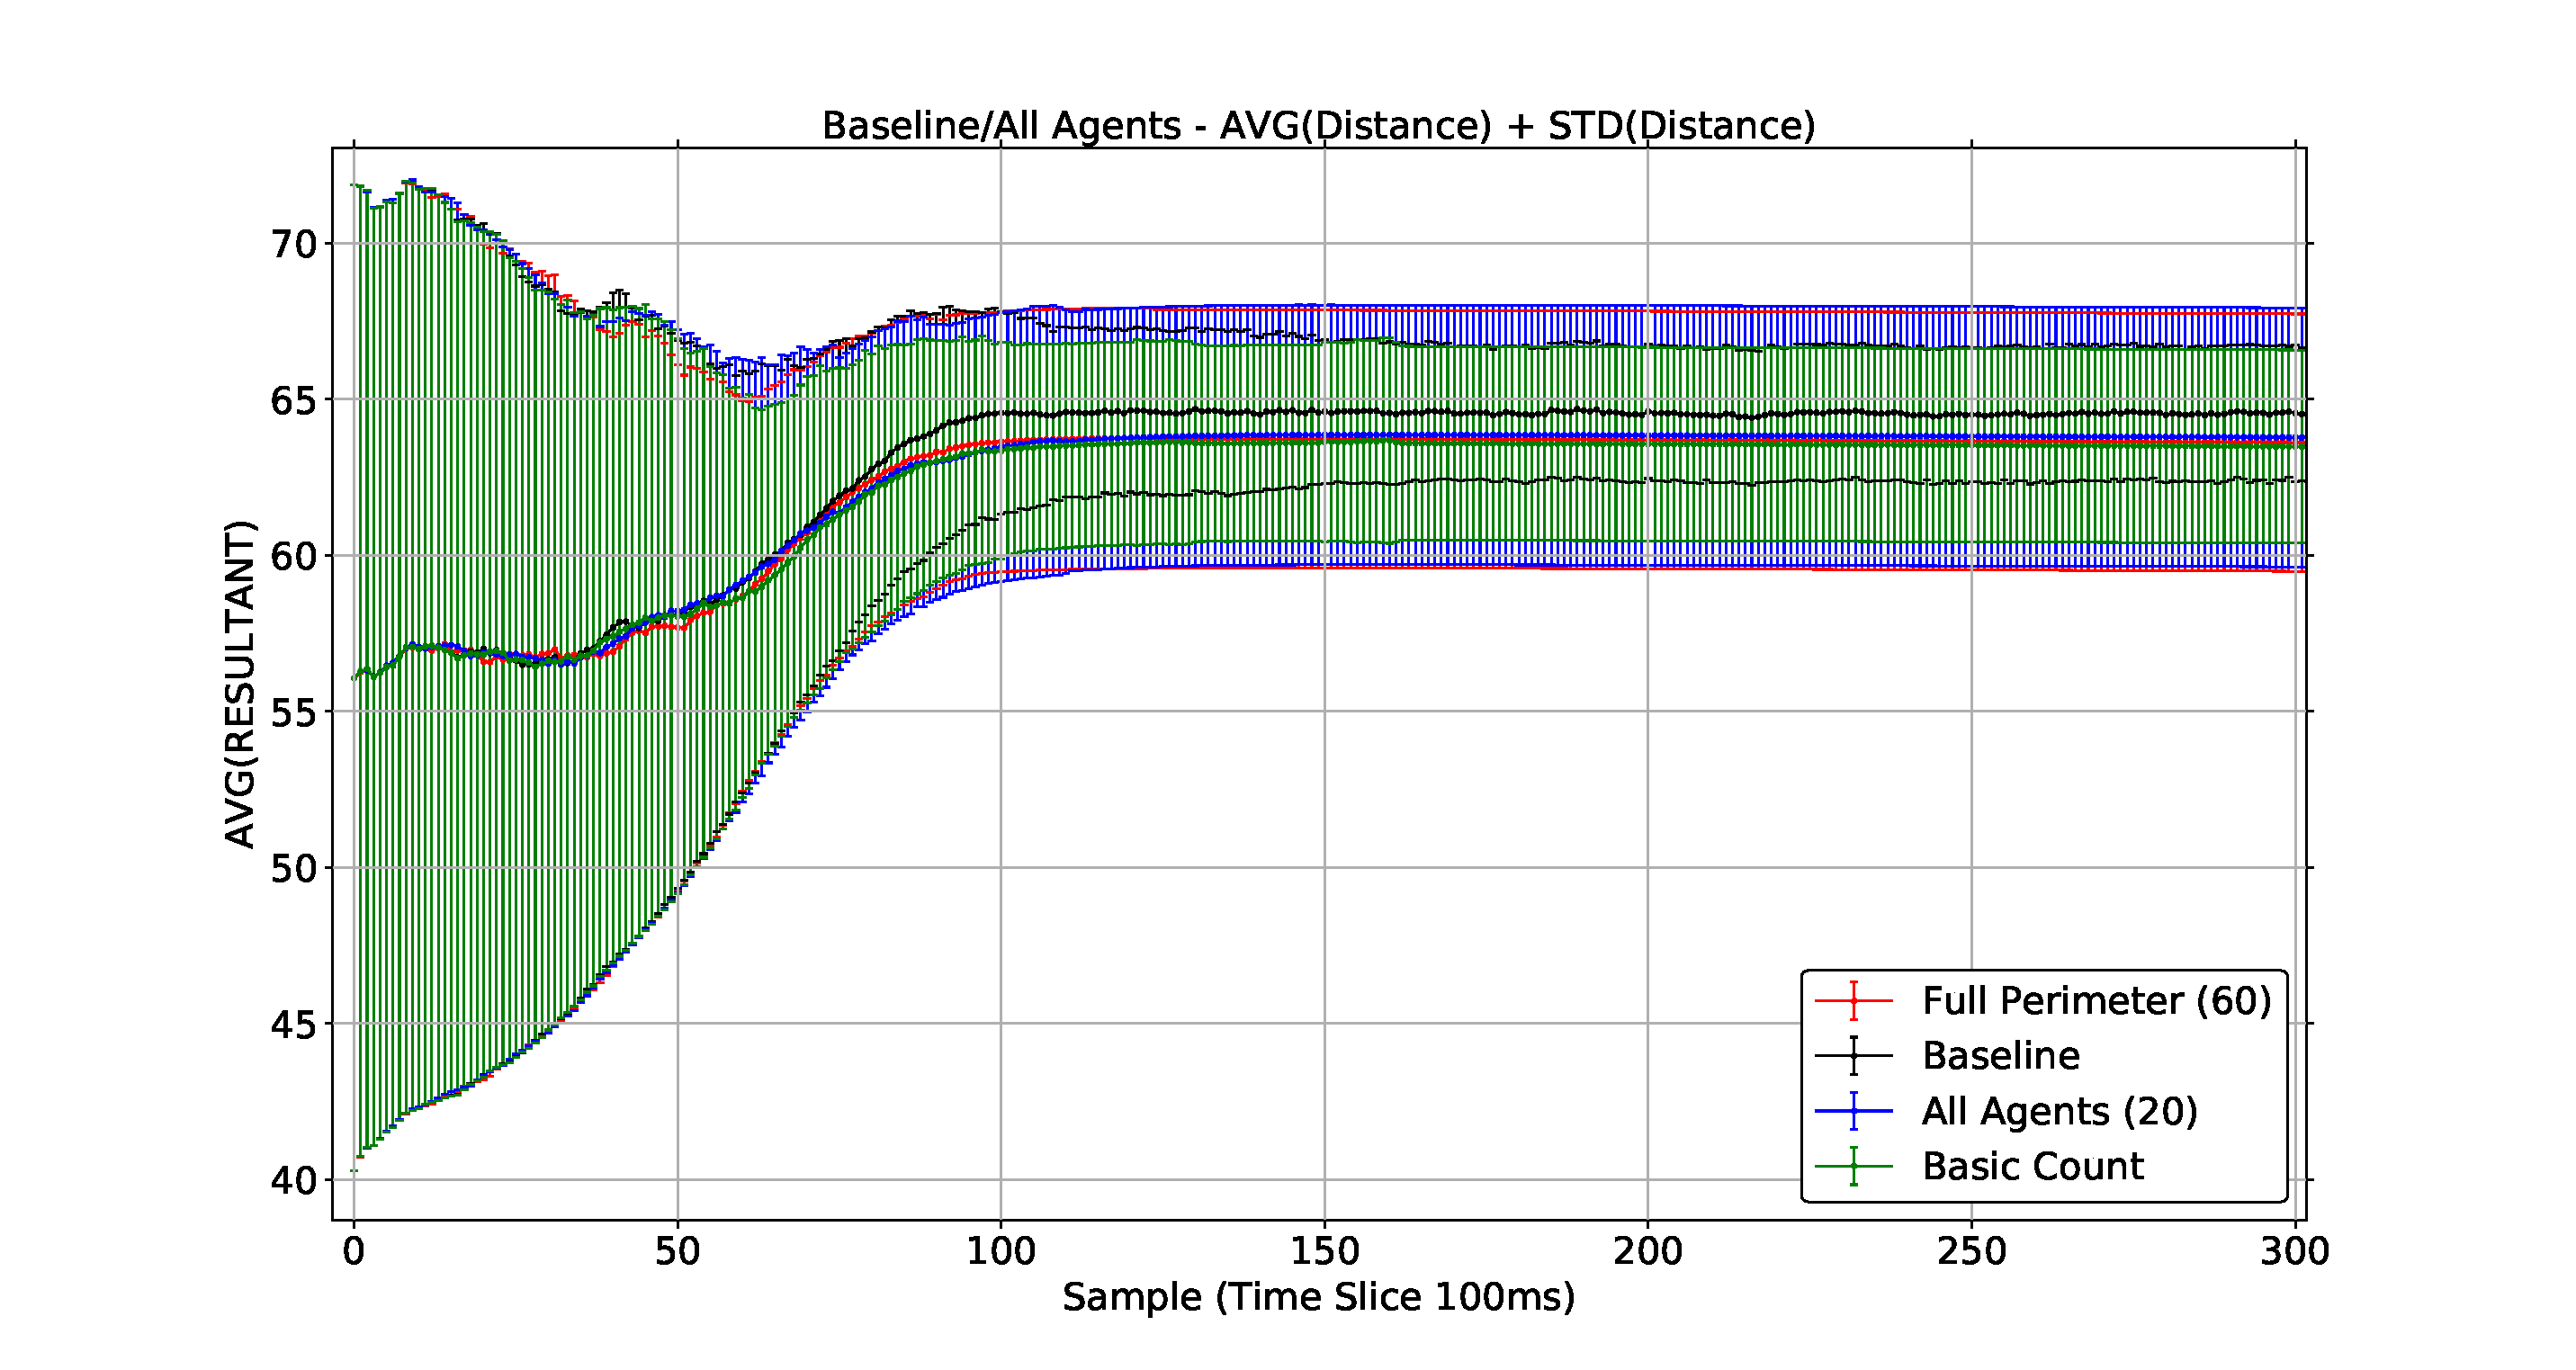
\includegraphics[width=14cm]{CHAPTER-6/figures/BaselineAll100-60-20-1}
\end{center}
\caption{Swarm distance analysis\label{fig:BaselineAll100-60-20-1}}
\end{figure}

Figure~\ref{fig:BaselineAll100-60-20-1} shows that the stabilisation periods of all the algorithms are much closer when the bias is proportional and the disorganised stage for all the algorithms appear to be reduced to be within the same time frame as the baseline.

\begin{figure}[H]
\begin{center}
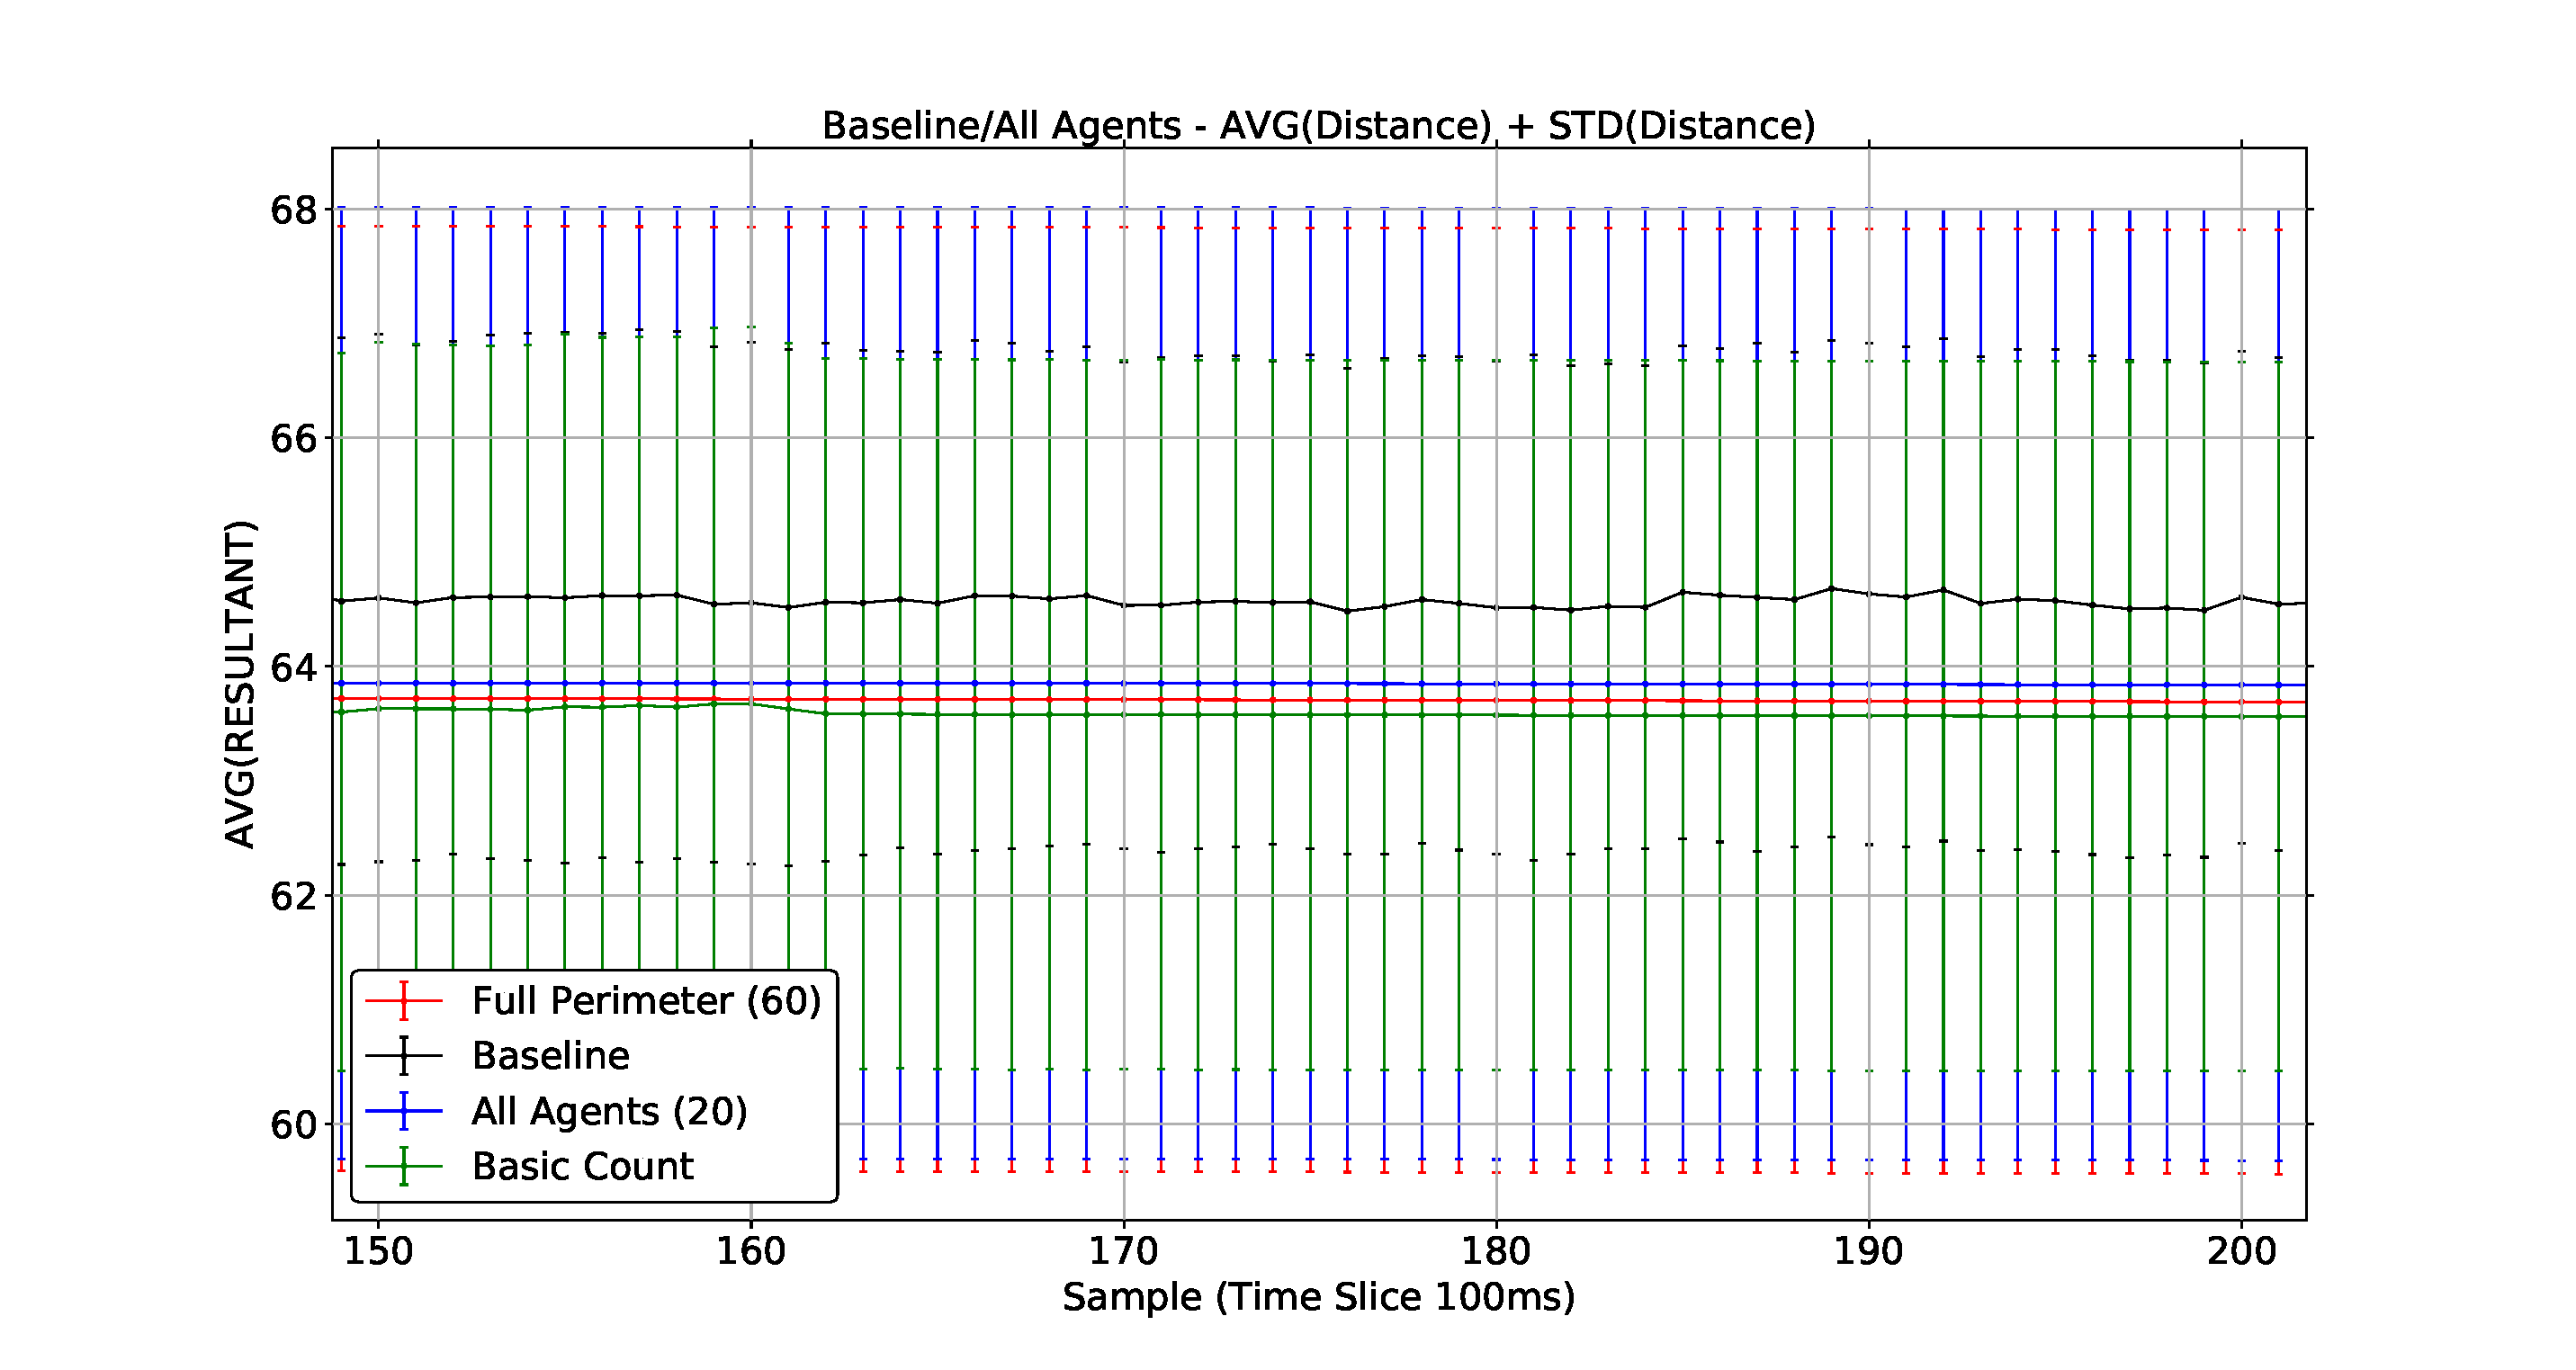
\includegraphics[width=14cm]{CHAPTER-6/figures/BaselineAll100-60-20-2}
\end{center}
\caption{Swarm distance analysis\label{fig:BaselineAll100-60-20-2}}
\end{figure}

Figure~\ref{fig:BaselineAll100-60-20-2} shows that the resultant distance is also very close and the deviations are also very close. These results indicate that it is possible to reduce the internal jitter that is caused by an algorithm by adjusting the bias to weighting to be proportional to the number of agents that apply the directional influence.

Figures \ref{fig:BaselineAllMag100-60-20-1} and \ref{fig:BaselineAllMag100-60-20-2} show that the magnitude is also affected by the balancing of the directional bias. \ref{fig:BaselineAllMag100-60-20-1} shows the disorganised phase with the rapid expansion with the negative magnitude. This if followed by the stable period. 

\begin{figure}[H]
\begin{center}
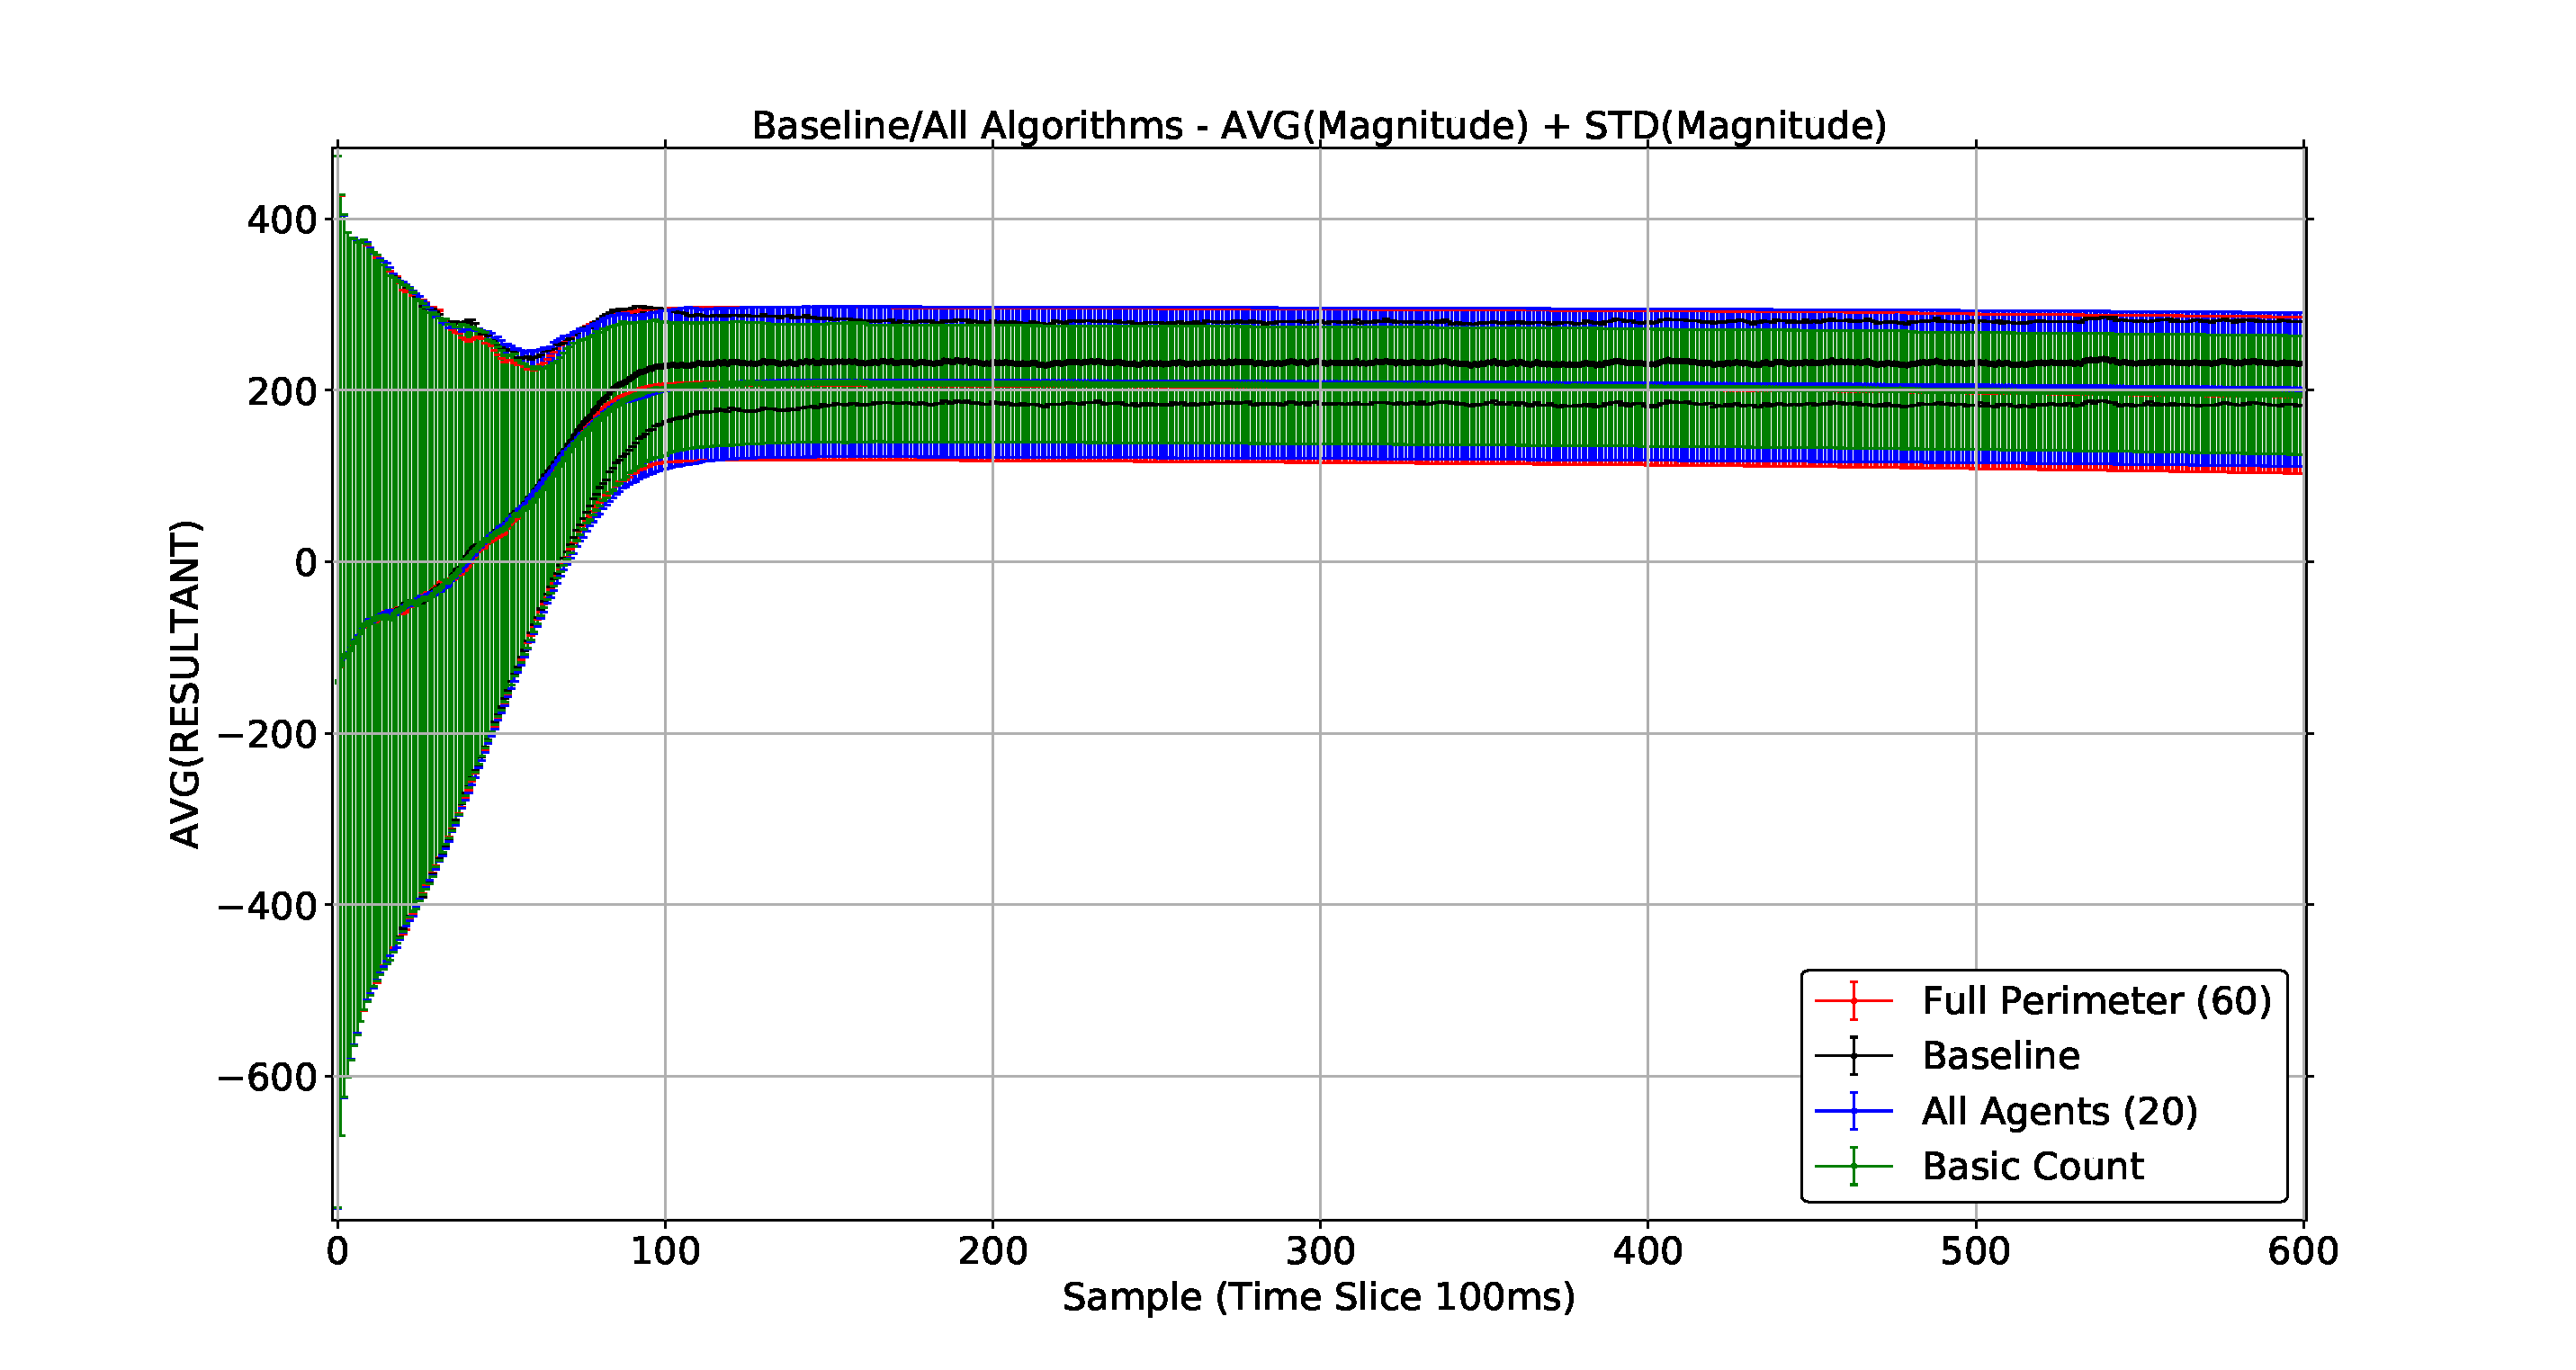
\includegraphics[width=14cm]{CHAPTER-6/figures/BaselineAllMag100-60-20-1}
\end{center}
\caption{Swarm magnitude analysis\label{fig:BaselineAllMag100-60-20-1}}
\end{figure}

\begin{figure}[H]
\begin{center}
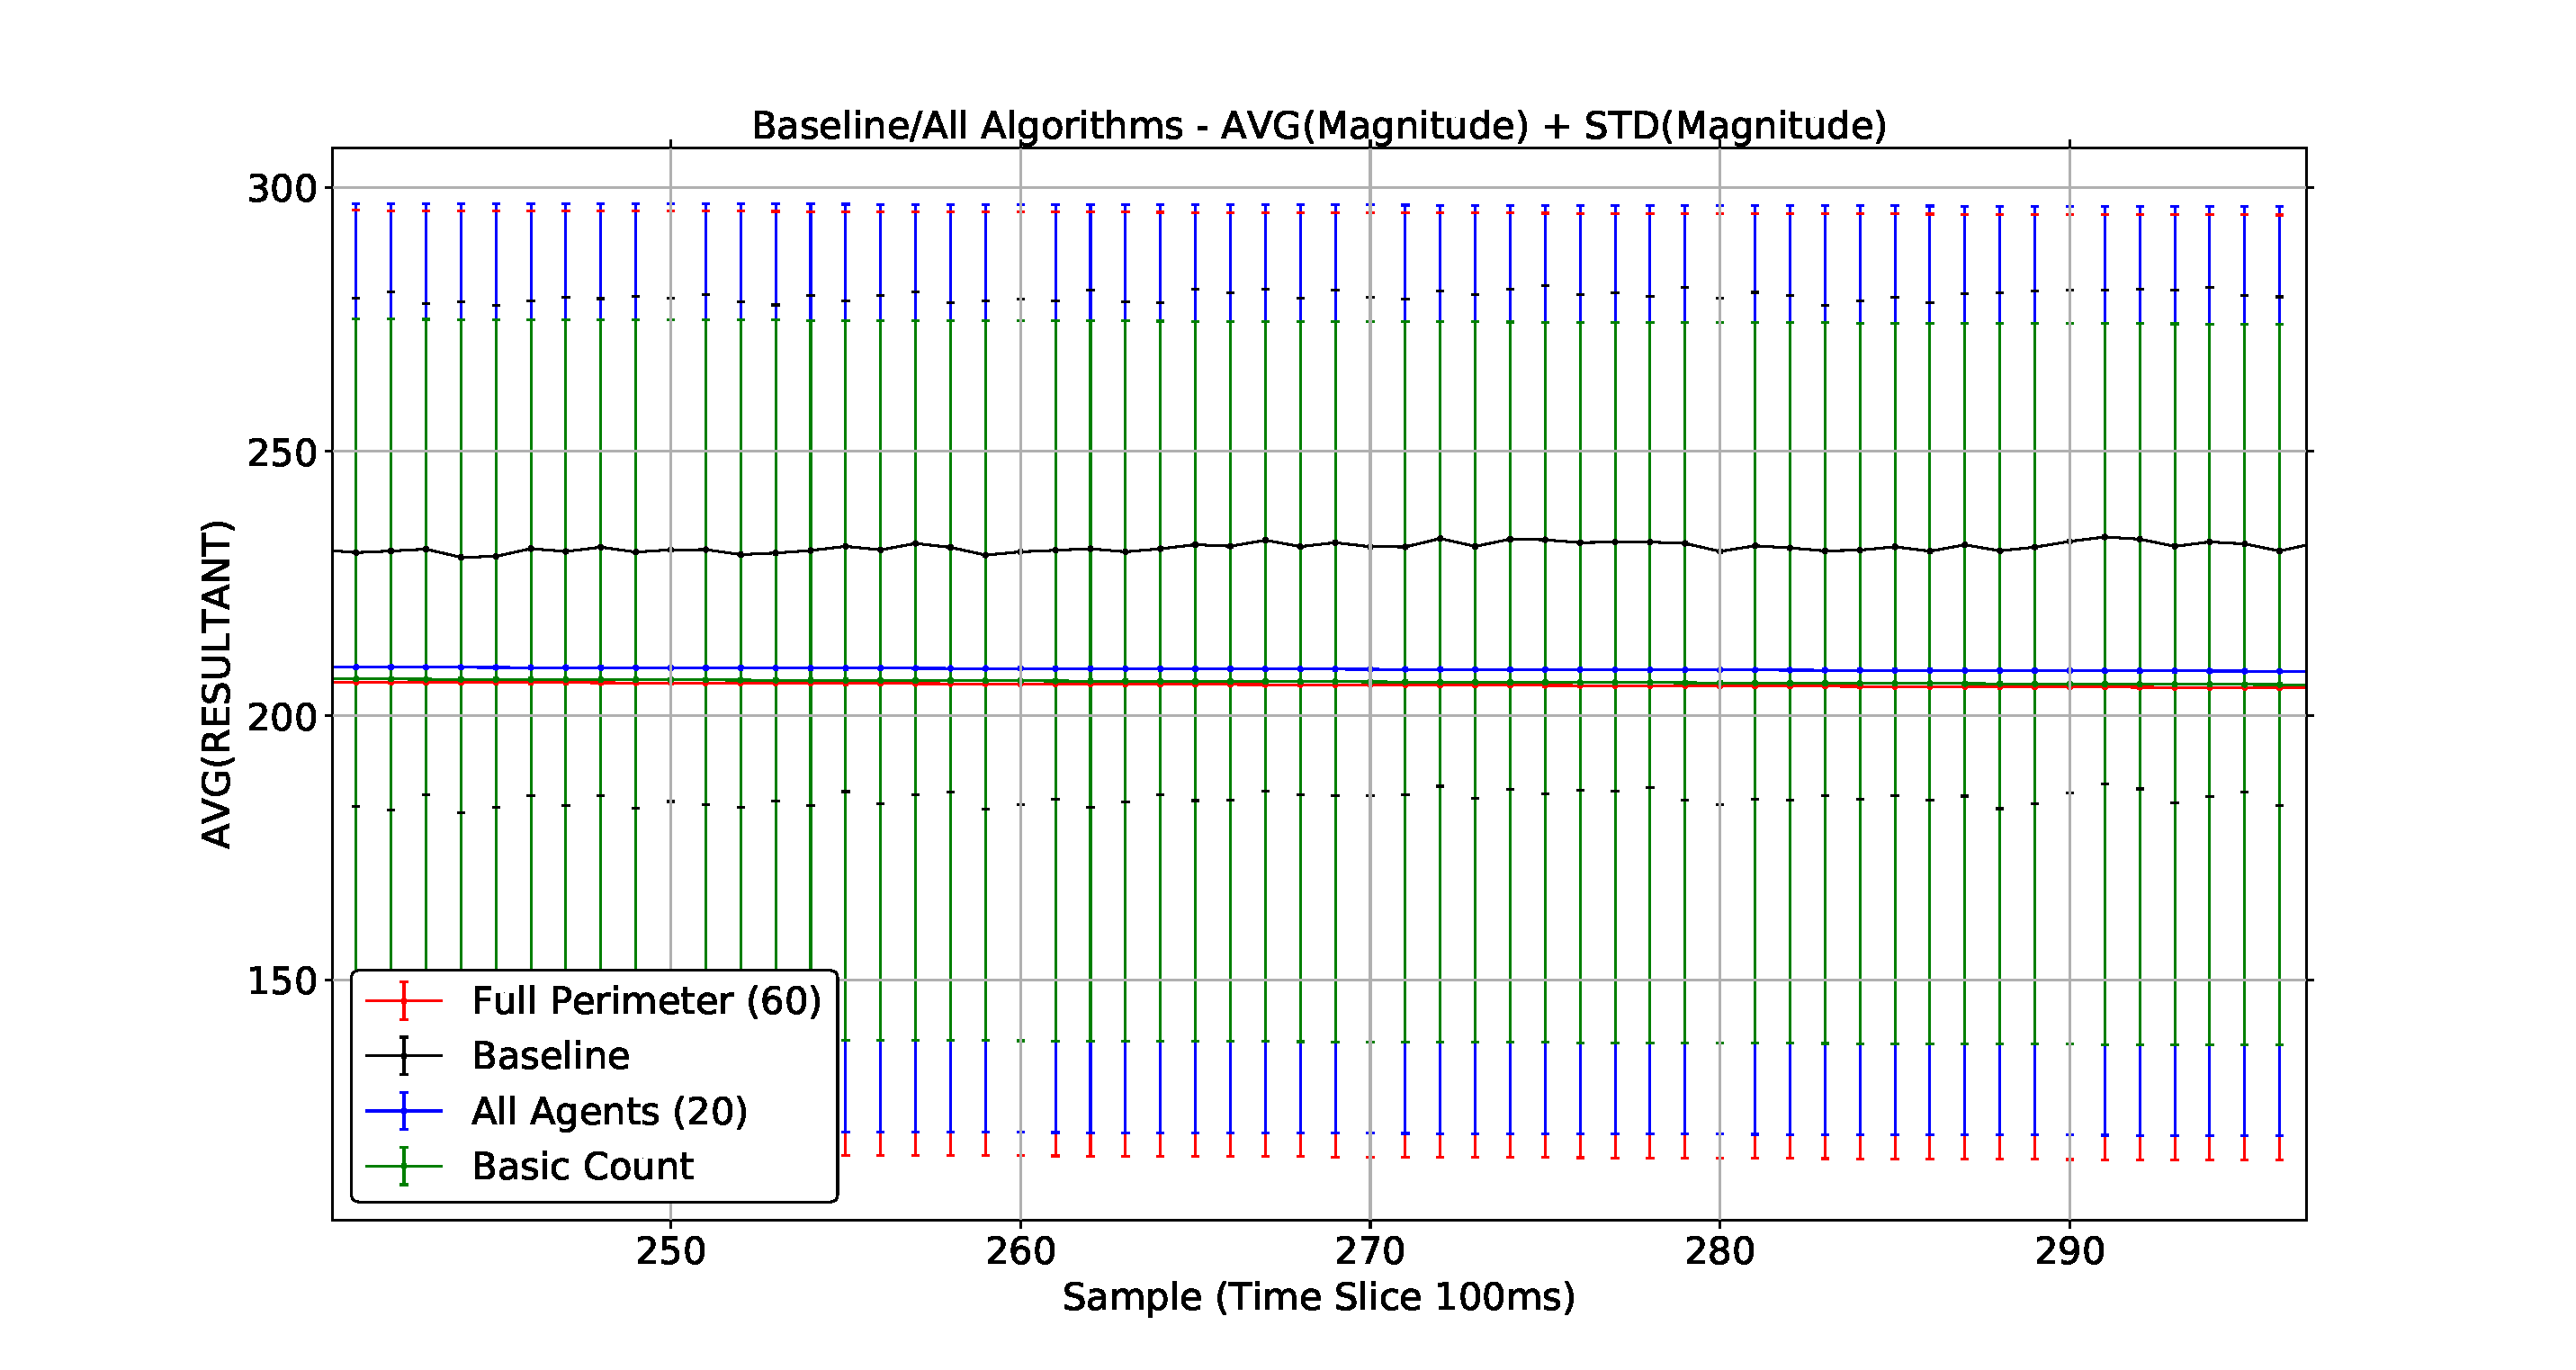
\includegraphics[width=14cm]{CHAPTER-6/figures/BaselineAllMag100-60-20-2}
\end{center}
\caption{Swarm magnitude analysis\label{fig:BaselineAllMag100-60-20-2}}
\end{figure}

Figure~\ref{fig:BaselineAllMag100-60-20-2} shows the balance with the inter-agent magnitude for all the algorithms at a very similar level. It is noticeable however that the basic-count algorithm still has the lowest jitter.

\begin{figure}[H]
\begin{center}
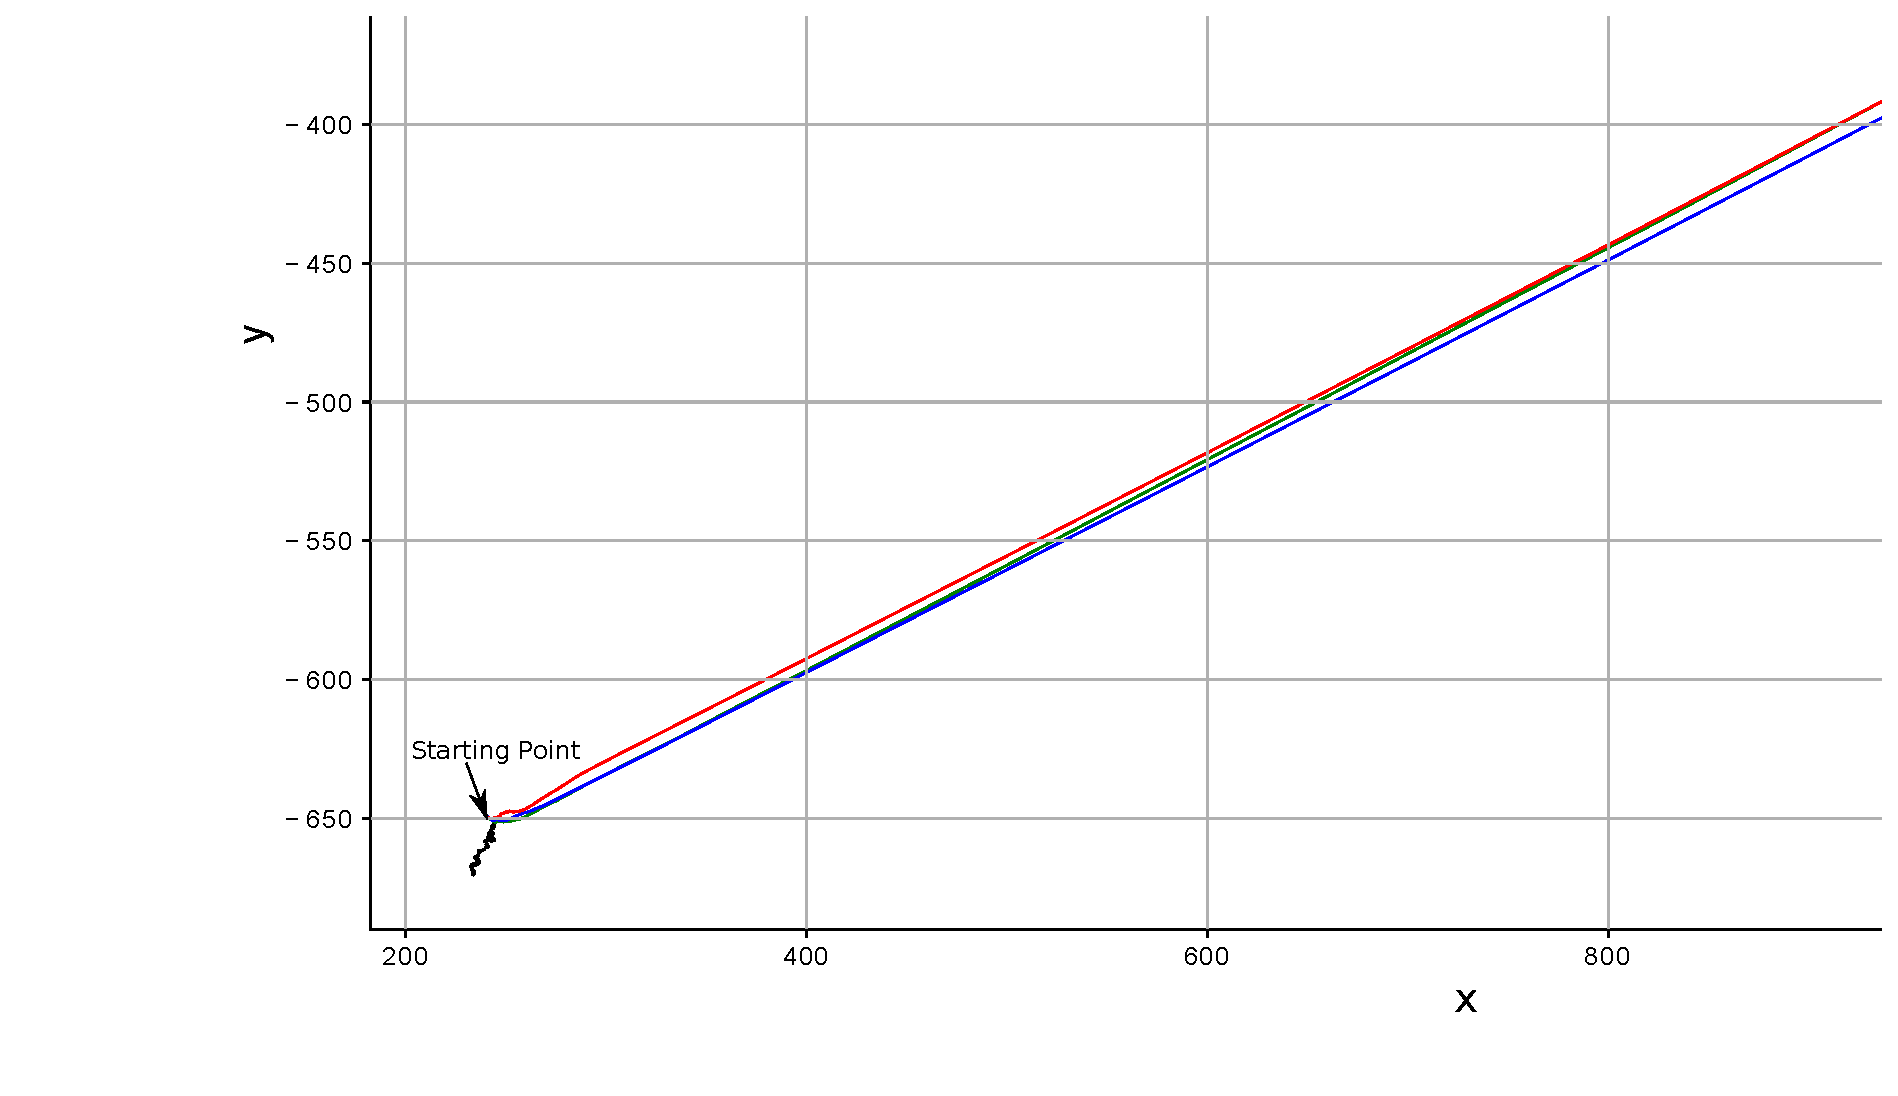
\includegraphics[width=14cm]{CHAPTER-6/figures/BaselineAllPath100-60-20-1}
\end{center}
\caption{Swarm path analysis\label{fig:BaselineAllPath100-60-20-1}}
\end{figure}

Figure~\ref{fig:BaselineAllPath100-60-20-1} shows that with the adjusted weightings the swarms still progress towards their goal. Figure~\ref{fig:BaselineAllPath100-60-20-2} shows that the reduced weightings impact on the directional path of the swarm and all the algorithms are effected by the \textit{interaction vector magnitudes} during the initial expansion disrupting the swarm path.

Figure~\ref{fig:BaselineAllPath100-60-20-3} shows that all the algorithms produce a goal-based swarm with the `all-agent' algorithm furthest progress towards the end point. This is due to the instant directional influence of the algorithm. 

\begin{figure}[H]
\begin{center}
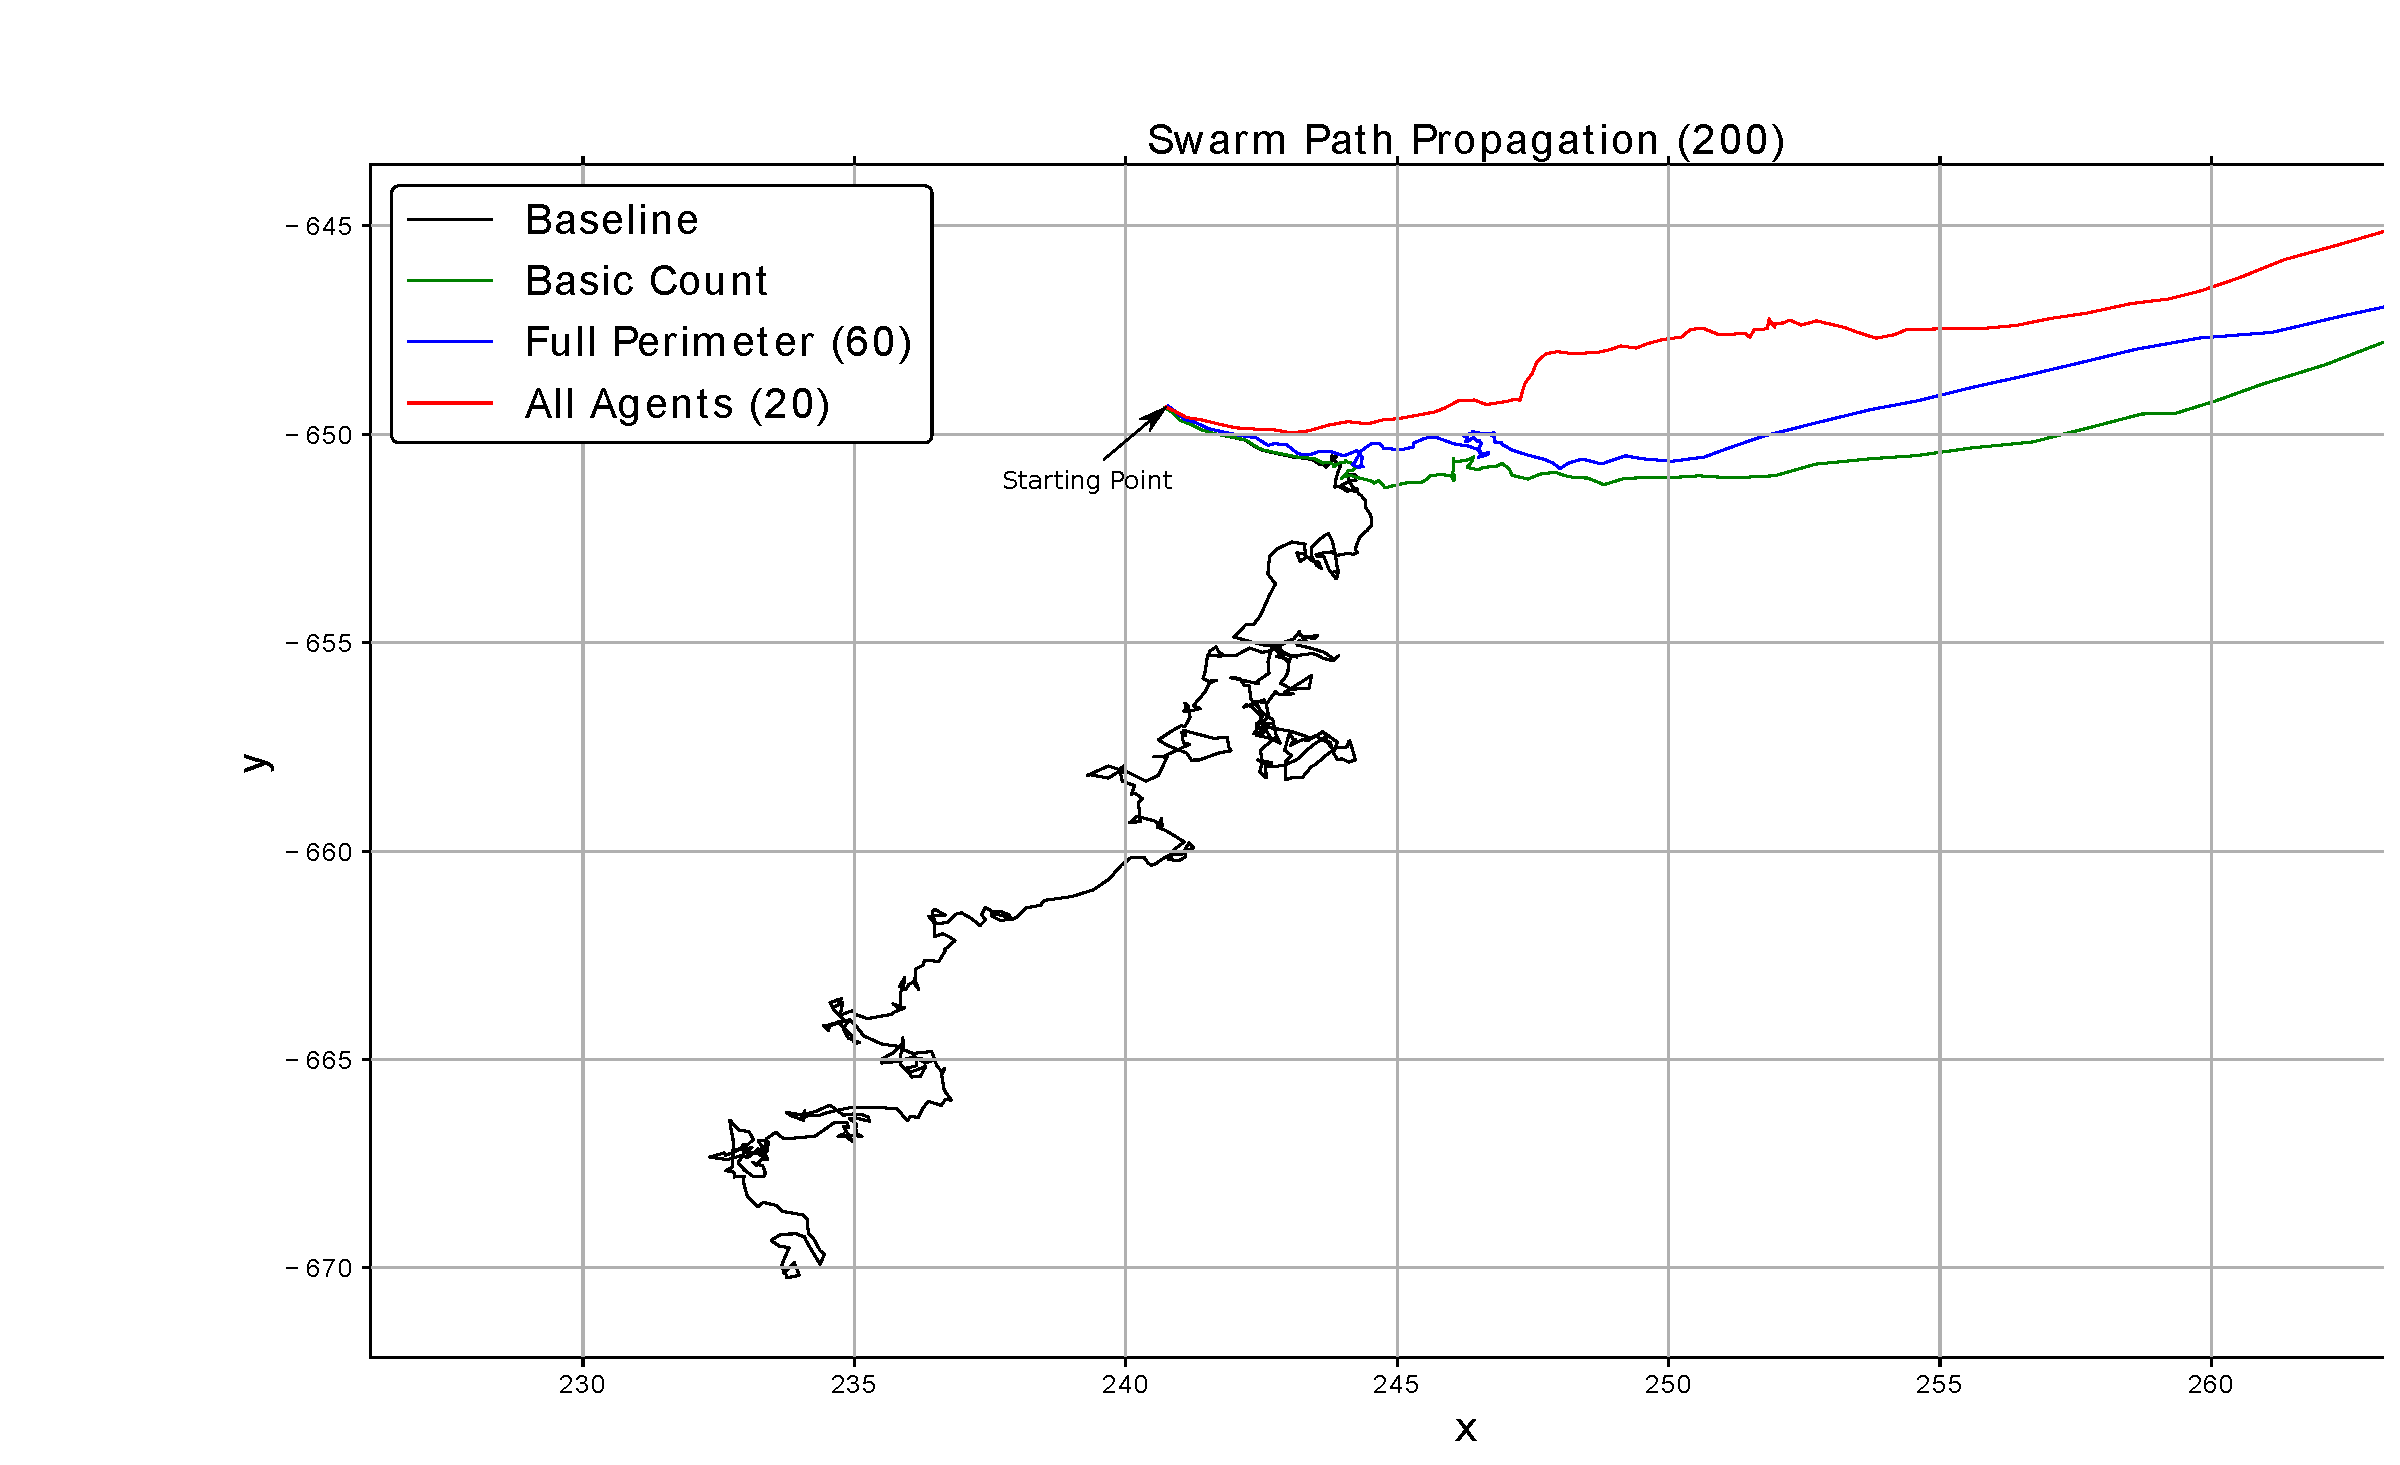
\includegraphics[width=14cm]{CHAPTER-6/figures/BaselineAllPath100-60-20-2}
\end{center}
\caption{Swarm path analysis\label{fig:BaselineAllPath100-60-20-2}}
\end{figure}

\begin{figure}[H]
\begin{center}
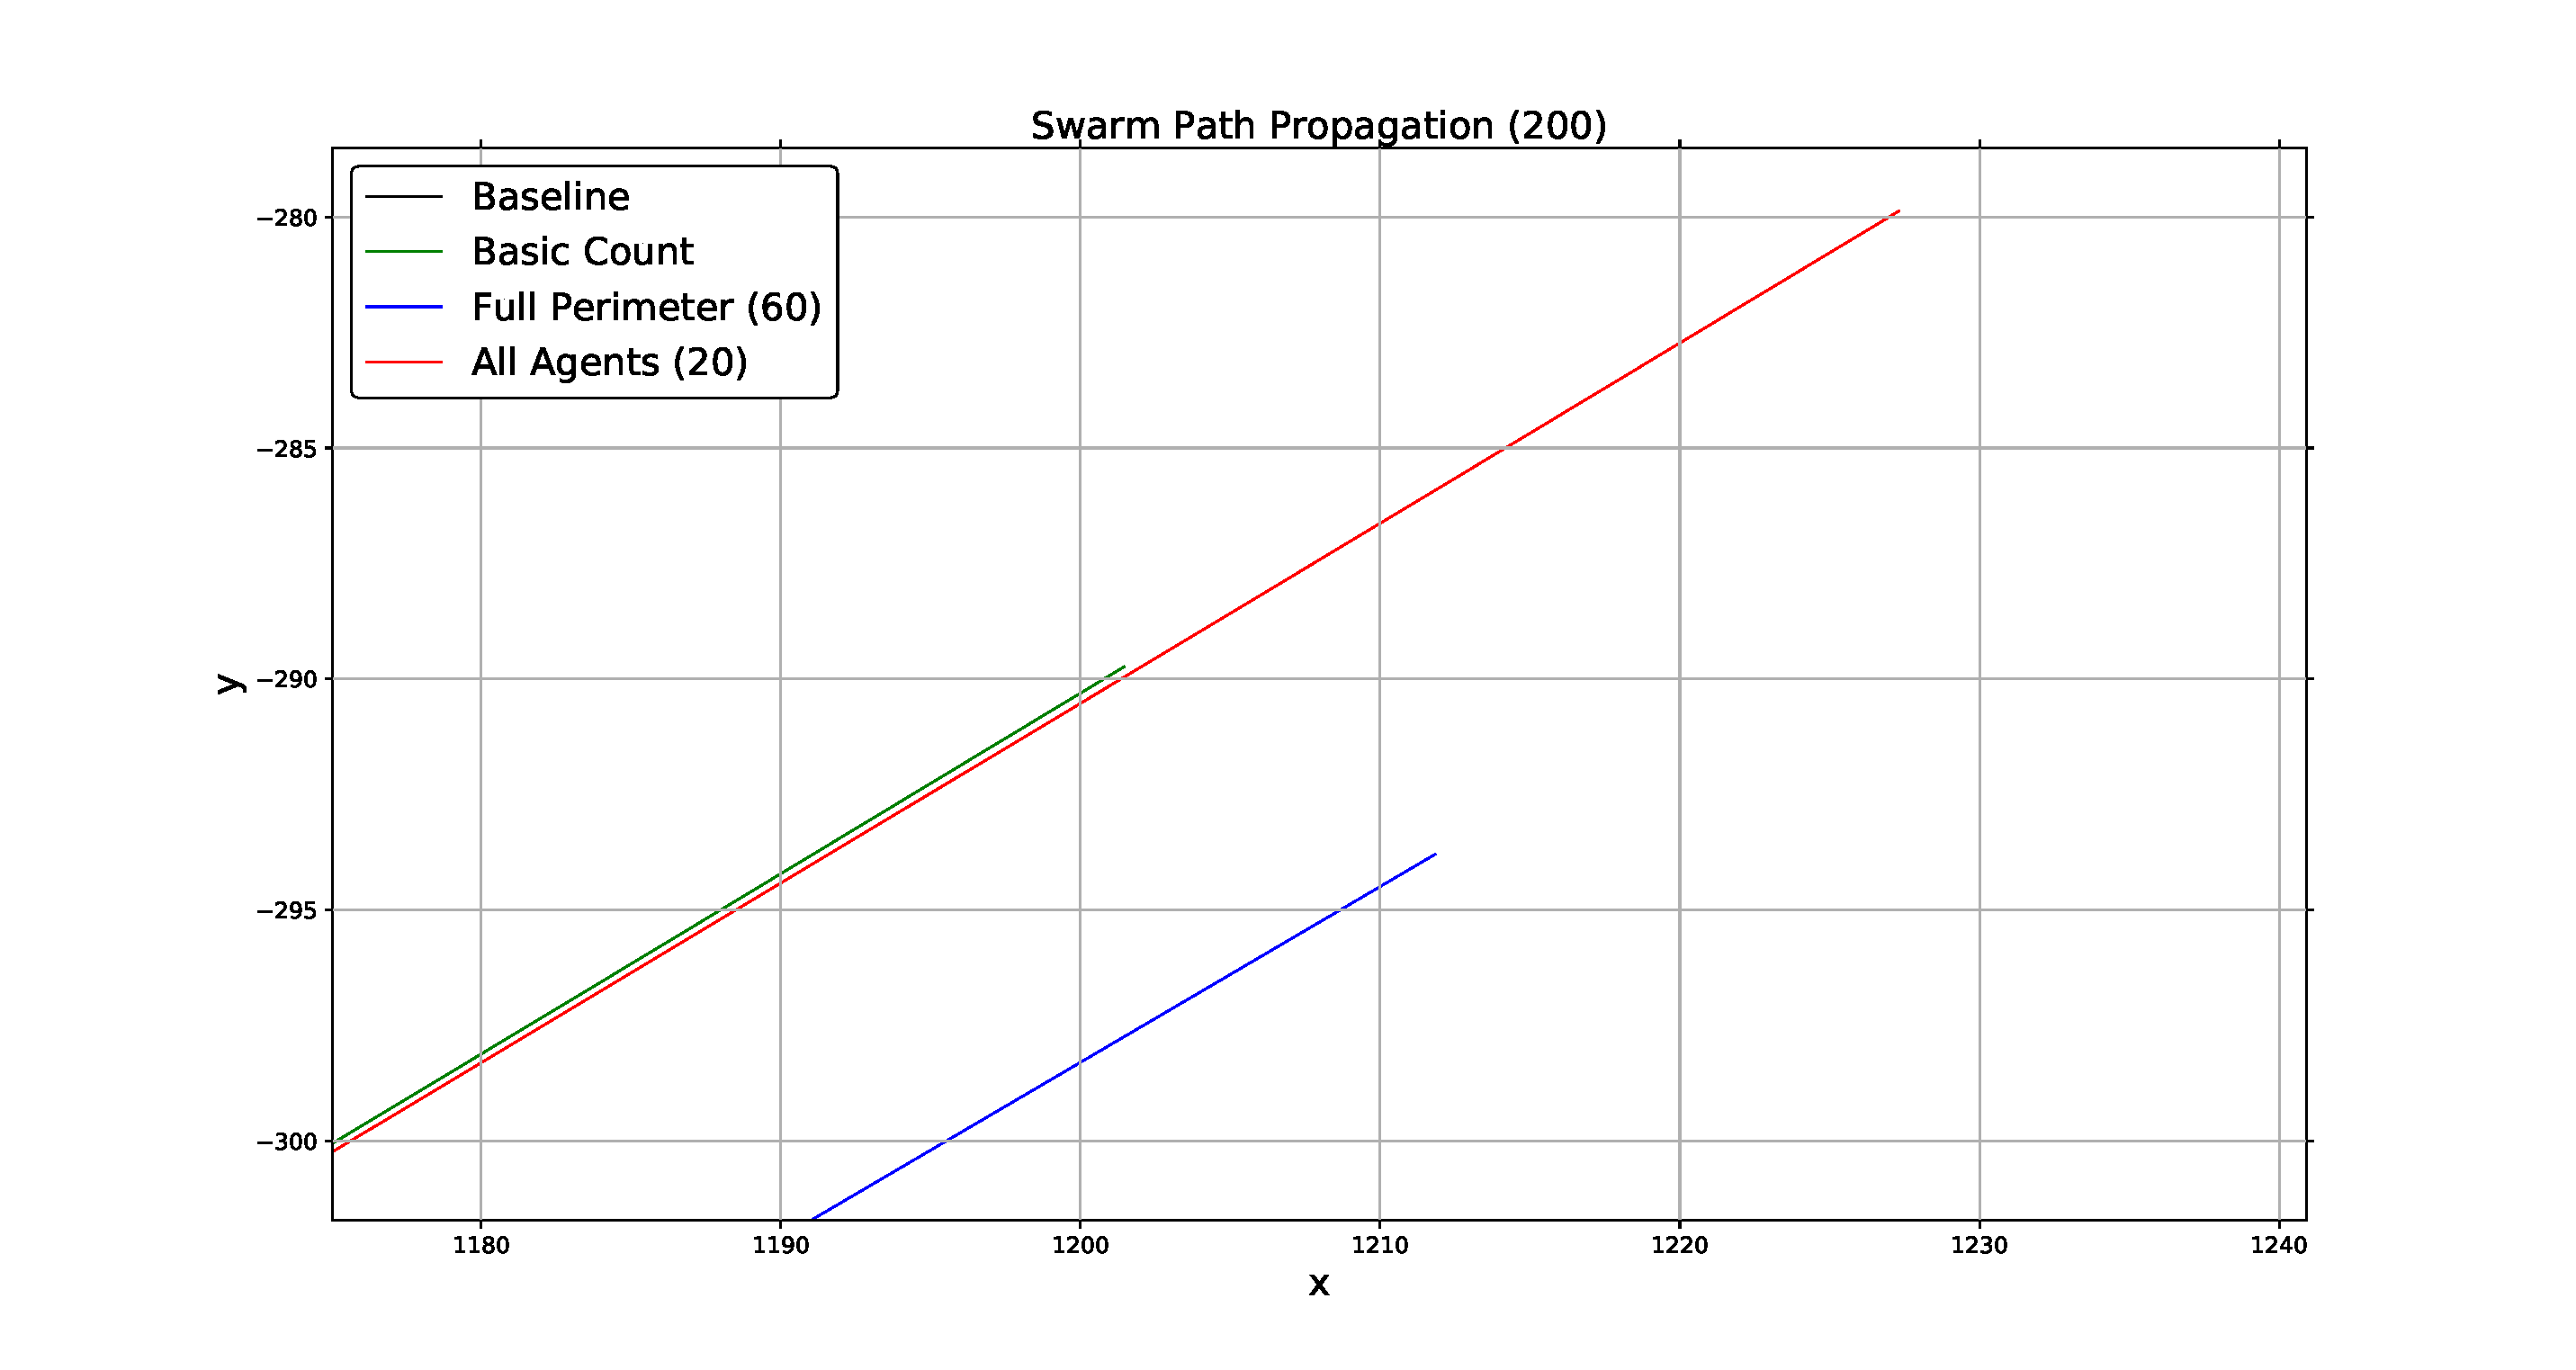
\includegraphics[width=14cm]{CHAPTER-6/figures/BaselineAllPath100-60-20-3}
\end{center}
\caption{Swarm path analysis\label{fig:BaselineAllPath100-60-20-3}}
\end{figure}

\subsection{Swarm coordination evaluation\label{reduced:coordinationEvaluation}}
Comparing the three metrics it is possible to determine the coordination effects based on the requirements of the swarm.

The resultant terminal speed of the swarm, based on the centroid, is minimally effected by the algorithm. 

The ability of the swarm to propagate towards a destination is hampered by reducing the number of coordinators as the stabilisation of the swarm's structure reduces the \textit{destination vector magnitude}. The most effected algorithm is the basic-count algorithm which is unable to influence the swarm at deployment due to compression reducing the number of coordinators and lessening the aggregate \textit{destination vector magnitude}. The full perimeter algorithm creates a greater aggregate \textit{destination vector} more quickly than the basic-count algorithm, however the algorithm does induce additional jitter. The `all-agent' algorithm has an immediate aggregate \textit{destination vector magnitude} but this algorithm also induces jitter such that the hexagonal lattice start to fail.
 
Increasing the number of coordinators increases the amount of internal disturbance within the swarm which can affect a sensor array in terms of its ability to function efficiently. Adjusting the weighting of $k_d$ can improve this as discussed in~\autoref{sec:AlternateBias1}. The algorithm that is most improved by adjusting the weightings is the `all-agent' algorithm such that it allows the hexagonal lattice to form and still produces an immediate directional bias through the aggregate \textit{destination vectors}.  

The computational overhead of each of the algorithms differs only in the logic that is required for swarm coordination. The is no computation overhead for the `all-agents` algorithm. The computational requirements of the basic-count algorithm is a simple count of neighbours and the full perimeter requires sweeps of angles and visibility checks which may impact on processor speeds for implementation. 

The main energy difference between the algorithms is the use of the GPS sensor which is a high energy consumption device. Therefore for general purpose coordination the basic-count algorithm provides the lowest GPS energy requirement and also minimal computational overhead.

\section{Energy efficiency evaluation\label{reduced:EnergyReductionGPS}}
The effect of an algorithm also effects the amount of gross energy that is used by the swarm in creating the directional effect. If we consider different size physical agents the overall effect of the algorithm can impact on the practical use of the swarm.

The following evaluation is based on analysing the motor and GPS usage and ignores the energy consumption of sensors and agent processor units.

Reducing the number of GPS modules being used at any point in time will impact the overall use of energy by the swarm. Comparing current GPS modules it was found that on average GPS modules consume approximately 44mA, for a 3.3V GPS. This equates to approximately 145mW of power as given by Ohm's Law. 

%% \begin{equation}
%% \label{eq:wattage}
%% W = V * I
%% \end{equation}

The energy usage of a motor will depend upon the power requirements required for agent movement (dependent on agent size and weight). It is assumed that the agents will utilise an omni-ball movement system to provide universal movement. Most omni-ball systems utilise 3 motors to control the movement~(Figure~\ref{fig:OmniBall}), other configuration are possible such as the four wheeled omni-directional wheelbase\cite{PD:06}.

\begin{figure}[H]
\begin{center}
\includegraphics[width=6cm]{CHAPTER-6/figures/OmniBall}
\end{center}
\caption{Omni-ball motor arrangement \label{fig:OmniBall}}
\end{figure}

Three possible scenarios of different motor requirements are compared for possible energy savings.

The three scenarios are for 3A, 1A and 400mA motors.

The scenario assumes a GPS is being used in all the agents as shown in~(Table~\ref{tab:GPSUsage}) the energy consumption will be based on a swarm size of 200 agents.

\begin{table}[H]
\begin{center}
%\fontsize{8}{8}\selectfont
\begin{tabular}{| r | r | r | r |}
\hline
Motor & Watts  & No GPS & With GPS \\ \hline
100mA &  0.33W &  0.99W & 1.1352W\\ \hline
1A    &  3.3W  &  9.90W & 10.0452W\\ \hline
3A    &  9.9W  & 29.70W & 29.8452W\\ \hline
\end{tabular}\caption{Energy consumption per agent} \label{tab:Energy1}
\end{center}
\end{table}

\begin{table}[H]
%\fontsize{8}{8}\selectfont
\begin{center}
\begin{tabular}{| c | r | r | r |}
\hline
{\parbox{2cm}{\centering Motor}} & {\parbox{2cm}{\centering All\\100/0}} & {\parbox{2cm}{\centering Full\\36/64}} & {\parbox{2cm}{\centering Basic \\20/80}} \\ \hline
100mA &  227.04W &  208.4544W &  203.808W\\ \hline
1A    & 2009.04W & 1990.4544W & 1985.808W\\ \hline
3A    & 5969.04W & 5950.4544W & 5945.808W\\ \hline
\end{tabular}\caption{Energy consumption of swarm} \label{tab:Energy2}
\end{center}
\end{table}

\begin{table}[H]
%\fontsize{8}{8}\selectfont
\begin{center}
\begin{tabular}{| c | r | r | r |}
\hline
{\parbox{2cm}{\centering Motor}} & {\parbox{2cm}{\centering All\\100/0}} & {\parbox{2cm}{\centering Full\\36/64}} & {\parbox{2cm}{\centering Basic \\20/80}} \\ \hline
100mA & 0\% & 8.186\% & 10.232\% \\ \hline
1A    & 0\% & 0.925\% &  1.156\% \\ \hline
3A    & 0\% & 0.311\% &  0.389\% \\ \hline
\end{tabular}\caption{Energy consumption of swarm} \label{tab:Energy3}
\end{center}
\end{table}

Tables~\ref{tab:Energy1}, \ref{tab:Energy2}~and~\ref{tab:Energy3} show the most effective savings in energy can be achieved by using smaller motors. This implies using smaller agents will provide the most appropriate platform to use GPS energy conservation. This efficiency saving falls in line with the current trend in using smaller agents in swarms as described by Mulgaonkar et al.~\cite{KV:16,MCK:15} who work as part of the research group at the University of Pennsylvania.

\section{Message Propagation Performance\label{methods:MessagePropogation}}
Many algorithms depend upon the propagation of messages throughout a swarm to determine many of the characteristics that allow it to be controlled~\cite{MD:09}. However message propagation has an ($O(n^2)$) propagation profile which effects the speed at which a swarm can react to characteristic changes~\cite{SHA:07}. This could be countered by a reduction in the speed that agents move within a swarm to counter the message propagation delays. 

The perimeter detection algorithms employed in this thesis have been reduced from ($O(n^2)$) to zero by limiting the agents information needs to simple proximity information from a sensor. This is a bio-inspired approach taken from the flocking of birds and shoaling of fish.

By reducing the message propagation to zero the scalability of the perimeter and void reduction algorithms are improved. Most research using message propagation techniques use swarms of at most 50 agents, as discussed this thesis is based upon the control of arbitrary sized swarms.

By localising the information requirements of an agent the storage requirements for message propagation are removed. Collating any characteristics of a swarm will require some form of local storage. As the messages propagate through a swarm more and more data is generated and data must be communicated and stored by each agent along with agent identifiers and some form of time stamp so data can be expired. In the case of the SenseSwarm algorithm this data is stored as a table of all agents, their coordinates, and a message id. This information is used to allows an agent to determine if it is at the lowest point in the swarm and therefore a perimeter agent~\cite{ZAPS:07}.

\subsection{SenseSwarm Message Propagation Comparison}
\begin{figure}[H]
\begin{center}
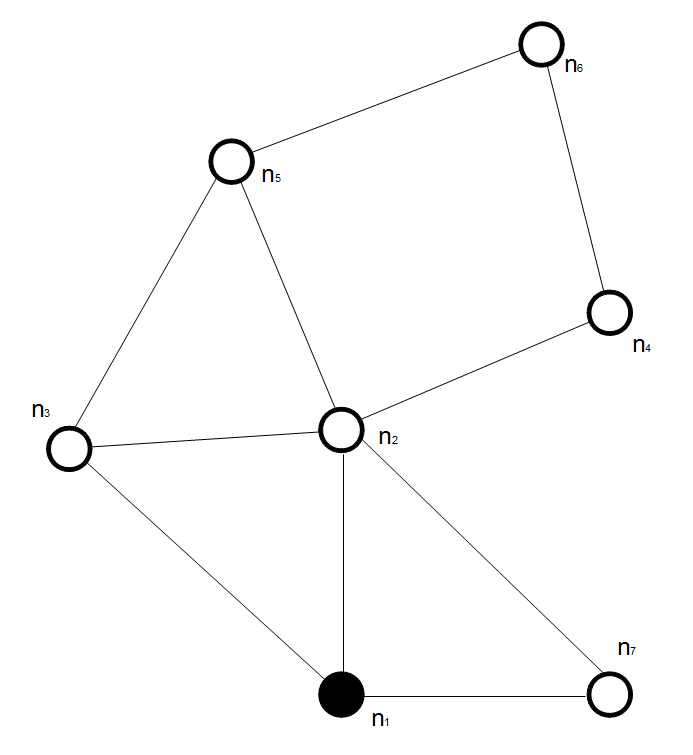
\includegraphics[width=6cm]{CHAPTER-6/figures/MessagePropogation1}
\end{center}
\caption{Message Propagation \label{methods:MessagePropogation1}}
\end{figure}

The SenseSwarm~\cite{ZAPS:07, APZDAMC:09, AZDPS:11} algorithm detects perimeters using a mechanism by which a lowest point in the swarm is identified. This is achieved by each agent collating a table of every agents coordinates. Each message consists of an `agent identifier' and a `message id'. The message is constructed by an agent and forwarded to each of its neighbours. If a message is received with the same `agent identifier' and `message id' as a previous message it is discarded. If the message is detected for the first time then the message is forwarded to all of the neighbour-agent's neighbours.

for $(n_1)$ the message propagation will be:-

$n_1 \to \{n_3, n_2, n_7\}$ \\
$n_3 \to \{n_2, n_5\}$\\
$n_7 \to \{n_2\}$\\
$n_2 \to \{n_5, n_4\}$\\
$n_5 \to \{n_6\}$\\
$n_4 \to \{n_6\}$\\

The SenseSwarm algorithm works by locating the lowest agent in the swarm and then that agent propagating a message left and right to next lowest neighbours to identify the swarm's outer edge. 

The SenseSwarm mechanism does not detect internal voids and is therefore not suitable for concave reduction as discussed in chapter~\ref{chapter:ConcaveReduction}.

\section{Conclusion\label{methods:Conclusion}}

This chapter discusses three techniques to create goal based swarms. The techniques are: using all the agents to coordinate a swarm, using perimeter agents only, and using a subset of the perimeter agents. 

The techniques are then analysed using the metrics defined in chapter~\ref{chapter:metric} to identify the effect the coordination techniques have upon the internal structures of the swarm.

Both metrics identify the state of a swarm with respect to variations in the disbursement of the agents from an average distribution and show that by reducing the number of coordinator agents it is possible to improve the internal distribution of agents within a swarm. The results showed that the effects the algorithms have upon the swarm's agents could be balanced to reduce internal disturbances but that balancing the proportional effect would not impact on the energy usage of the positional sensors. 

The chapter also discusses the removal of an internal communications architecture and introduces a proximity-based approach that allows for arbitrary sized swarms to be goal based. 

